% ============================================================
%  main.tex  –  Master driver file
%  Compile ONLY this file in Overleaf (set as Main Document)
% ============================================================

\documentclass[12pt,a4paper,oneside]{report}

\usepackage[utf8]{inputenc}
\usepackage{acronym}
\usepackage[T1]{fontenc}
\usepackage{adjustbox} % add to preamble
\usepackage{microtype}  % prevents overfull hboxes / text overflow
\usepackage{times}
\usepackage{geometry}
\geometry{top=2.5cm, bottom=2.5cm, left=3.5cm, right=2.5cm}
\usepackage{graphicx}
% Images are in the local Images/ subfolder
\graphicspath{
  {Images/}
  {../YOLOv8-Path-Segmentation-RealTime-Optimization/Results/benchmark_results/}
  {../YOLOv8-Path-Segmentation-RealTime-Optimization/Results/inference_results/}
}
% Allow LaTeX to handle filenames with unusual extensions or spaces
\usepackage{grffile}
% Treat .jfif files as JPEG (same binary format, different extension)
\DeclareGraphicsRule{.jfif}{jpg}{.jfif}{}
\usepackage{amsmath,amssymb,amsfonts}
\usepackage{setspace}
\onehalfspacing
\usepackage{booktabs}
\usepackage{longtable}
\usepackage{array}
\usepackage{multirow}
\usepackage{ragged2e}
\usepackage{tabularx}
\usepackage{enumerate}
\usepackage{enumitem}
\usepackage{caption}
\captionsetup{justification=centering, font=small}
\usepackage{url}
\usepackage{placeins}
\usepackage{cite}
\usepackage{parskip}
\usepackage{titlesec}
\usepackage[linesnumbered,ruled,vlined]{algorithm2e}

\titleformat{\chapter}[block]
  {\normalfont\LARGE\bfseries\centering}{\thechapter}{1em}{}
\titlespacing*{\chapter}{0pt}{-10pt}{20pt}
\titleformat{\section}{\normalfont\large\bfseries}{\thesection}{1em}{}
\titleformat{\subsection}{\normalfont\normalsize\bfseries}{\thesubsection}{1em}{}
\titleformat{\subsubsection}{\normalfont\normalsize\itshape}{\thesubsubsection}{1em}{}

% hyperref MUST be last
\usepackage[
  bookmarks=true,
  colorlinks=true,
  linkcolor=black,
  citecolor=black,
  urlcolor=blue,
  pdfborder={0 0 0},
  pdftitle={Implementation of a Communication-Integrated Mobile Environmental Monitoring Framework},
  pdfauthor={Satwik Shreshth}
]{hyperref}

\setcounter{tocdepth}{3}
\setcounter{secnumdepth}{3}

% Front-matter unnumbered chapter heading
\newcommand{\fmchapter}[1]{%
  \clearpage\phantomsection
  \begin{center}{\LARGE\bfseries #1}\end{center}
  \vspace{0.5cm}
  \addcontentsline{toc}{chapter}{#1}%
}

% ============================================================
\begin{document}
\renewcommand\bibname{References}
\pagenumbering{roman}

% ══════════════════════════════════════════════
%  TITLE PAGE
% ══════════════════════════════════════════════
\begin{titlepage}
\newgeometry{top=2cm, bottom=2cm, left=2.5cm, right=2.5cm}
\begin{center}

{\Large\bfseries Implementation of a Communication-Integrated Mobile\\[0.2cm]
Environmental Monitoring Framework}

\vspace{0.5cm}

{\large A Dissertation Report}

\vspace{0.3cm}

{\itshape Submitted in partial fulfillment of\\[0.2cm]
the requirements for the award of the degree of}

\vspace{0.3cm}

{\large\bfseries Master of Computer Applications}

\vspace{0.5cm}

{\large Submitted by}

\vspace{0.1cm}

{\large\bfseries Satwik Shreshth}\\[0.2cm]
{\normalsize Roll No: 24MCA014}

\vspace{0.5cm}

{\normalsize Under Guidance of}

\vspace{0.1cm}

{\normalsize\bfseries Mr.\ Partha Pratim Ray}\\[0.2cm]
{\normalsize Assistant Professor}\\[0.1cm]
{\normalsize Department of Computer Applications}\\[0.1cm]
{\normalsize Sikkim University}

\vspace{0.4cm}

{\normalsize Under the Co-Guidance of}

\vspace{0.001cm}

{\normalsize\bfseries Dr.\ Ravi Kant Jain}\\[0.2cm]
{\normalsize Scientist F, Intelligent Systems Engineering Group}\\[0.1cm]
{\normalsize CSIR--Central Mechanical Engineering Research Institute (CSIR-CMERI)}

\vspace{0.6cm}

\includegraphics[height=2.5cm]{SU_logojfif.jfif}
\hspace{2cm}
\includegraphics[height=2.5cm]{CMERI_logo.jfif}

\vspace{0.4cm}

{\large\bfseries Department of Computer Applications}\\[0.1cm]
{\large\bfseries Sikkim University}\\[0.1cm]
{\large\bfseries Gangtok-737102, India}

\end{center}
\restoregeometry
\end{titlepage}
% ══════════════════════════════════════════════
%  DEDICATION
% ══════════════════════════════════════════════
\newpage
\thispagestyle{plain}
\vspace*{\fill}
\begin{center}
{\itshape\large
  Inscribed to my parents, \textbf{Priya Tiwari} and \textbf{Ashok Kumar Tiwary},
  whose sacrifices paved my path,\\
  and sanctified by the grace of \textbf{Bhagwan Ram},
  the divine strength that guided this work to completion.}
\end{center}
\vspace*{\fill}
\phantomsection
\addcontentsline{toc}{chapter}{Dedication}

% ══════════════════════════════════════════════
%  ACKNOWLEDGEMENTS
% ══════════════════════════════════════════════
\newpage
\thispagestyle{plain}
\fmchapter{Acknowledgements}

{\setstretch{1.3}
\noindent
I am deeply grateful to \textbf{Mr.\ Partha Pratim Ray}, Assistant Professor,
Department of Computer Applications, Sikkim University, for his guidance,
encouragement, and the intellectual freedom he extended to me throughout this
research. His mentorship has been invaluable in shaping this work.

\vspace{0.45cm}
\noindent
I would like to express my sincere gratitude to \textbf{Dr.\ Ravi Kant Jain},
Scientist F, Intelligent Systems Engineering Group, Central Scientific and Industrial Research~-- Central Mechanical
Engineering Research Institute, Durgapur, for his expert guidance and for
providing access to the advanced laboratory facilities and technical infrastructure
at the institute. I am also thankful to \textbf{Dr.\ Naresh Chandra Murmu},
Director, Central Scientific and Industrial Research~-- Central Mechanical Engineering Research Institute, for the opportunity to carry out part of my dissertation
work at such a distinguished institution.

\vspace{0.45cm}
\noindent
I extend my gratitude to the \textbf{Head of Department} and all the faculty
members of the Department of Computer Applications, Sikkim University, for their
constructive feedback and continued academic support throughout my research.

\vspace{0.45cm}
\noindent
I also wish to thank the administrative and technical staff, as well as my fellow
research scholars at both Sikkim University and the Intelligent Systems Engineering Group of the Central Scientific and Industrial Research~-- Central Mechanical Engineering Research Institute, for their
cooperation, camaraderie, and collaborative spirit.

\vspace{0.45cm}
\noindent
I am sincerely thankful to my friends, \textbf{Pragya Sharma} and
\textbf{Suveer Kumar}, for their constant support, encouragement, and for making
this journey truly memorable.

\vspace{0.45cm}
\noindent
Finally, I am forever indebted to my parents, \textbf{Shree Ashok Kumar Tiwary}
and \textbf{Smt.\ Priya Tiwari}, whose unconditional love, sacrifices, and
blessings have been the bedrock of everything I have accomplished. This work would
not have been possible without them.

\vspace{1.8cm}
\begin{flushright}
Satwik Shreshth\\
Roll No: 24MCA014
\end{flushright}
}
% ══════════════════════════════════════════════
%  DECLARATION
% ══════════════════════════════════════════════
\newpage
\thispagestyle{plain}
\fmchapter{Declaration}

\noindent
I, \textbf{Satwik Shreshth}, Roll No.\ \textbf{24MCA014}, a student of the 4th
semester of the Master of Computer Applications at Sikkim University, Gangtok,
declare that this research is my original work, contains no unauthorized
third-party copyrighted material, and has not been submitted elsewhere for any
academic qualification.

\vspace{0.6cm}
\noindent
Any third-party material included has been appropriately handled by referencing
 with URLs provided where possible.

\vspace{3cm}
\begin{flushright}
Satwik Shreshth\\
Roll No: 24MCA014\\[0.4cm]
Date:\underline{\hspace{4cm}}
\end{flushright}
% ══════════════════════════════════════════════
%  CERTIFICATE FROM SUPERVISOR
% ══════════════════════════════════════════════
\newpage
\thispagestyle{plain}
\fmchapter{Certificate from Supervisor}

\noindent
This is to certify that \textbf{Mr.\ Satwik Shreshth}, Roll No.\ \textbf{24MCA014},
a student of the 4th Semester of Master of Computer Applications, is a registered
candidate under the Department of Computer Applications, Sikkim University, Gangtok.

\vspace{0.6cm}
\noindent
The undersigned certifies that the candidate has completed all requirements for the
submission of the dissertation entitled \textbf{``Implementation of a
Communication-Integrated Mobile Environmental Monitoring Framework.''} This work was
carried out under my supervision and guidance, in collaboration with CSIR-CMERI, Durgapur.

\vspace{0.6cm}
\noindent
I hereby recommend the acceptance of this dissertation in partial fulfillment of the
requirements for the award of the Degree of Master of Computer Applications.

\vspace{3cm}
\begin{flushright}
\textbf{Mr.\ Partha Pratim Ray}\\
Assistant Professor\\
Department of Computer Applications\\
Sikkim University, Gangtok, India\\[0.4cm]
Date:\underline{\hspace{4cm}}
\end{flushright}
% ══════════════════════════════════════════════
%  CERTIFICATE FROM CO-SUPERVISOR
% ══════════════════════════════════════════════
\newpage
\thispagestyle{plain}
\fmchapter{Certificate from Co-Supervisor}

\noindent
This is to certify that \textbf{Mr.\ Satwik Shreshth}, Roll No.\ \textbf{24MCA014},
a student of the 4th Semester of Master of Computer Applications at Sikkim
University, has successfully carried out his dissertation research at the Intelligent
Systems Engineering Group, CSIR--Central Mechanical Engineering Research Institute
(CSIR-CMERI), Durgapur.

\vspace{0.6cm}
\noindent
The research presented in the dissertation entitled \textbf{``Implementation of a
Communication-Integrated Mobile Environmental Monitoring Framework''} was conducted
under my co-supervision. I certify that the candidate has fulfilled
all the technical and academic requirements for the submission of this work.

\vspace{0.6cm}
\noindent
I hereby recommend the acceptance of this dissertation in partial fulfillment of the
requirements for the award of the Degree of Master of Computer Applications.

\vspace{3cm}
\begin{flushright}
\textbf{Dr.\ Ravi Kant Jain}\\
Scientist `F'\\
Intelligent Systems Engineering Group\\
CSIR-CMERI, Durgapur, India\\[0.4cm]
Date:\underline{\hspace{4cm}}
\end{flushright}

% ══════════════════════════════════════════════
%  CERTIFICATE FROM HEAD OF DEPARTMENT
% ══════════════════════════════════════════════
\newpage
\thispagestyle{plain}
\fmchapter{Certificate from Head of Department}

\noindent
This is to certify that \textbf{Mr.\ Satwik Shreshth}, Roll No.\ \textbf{24MCA014},
a student of the 4th Semester of the Master of Computer Applications programme,
has satisfactorily completed his dissertation work under the supervision of
\textbf{Mr.\ Partha Pratim Ray}, Assistant Professor, Department of Computer
Applications, Sikkim University, and under the co-supervision of
\textbf{Dr.\ Ravi Kant Jain}, Scientist F, Intelligent Systems Engineering Group,
CSIR--Central Mechanical Engineering Research Institute (CSIR-CMERI), Durgapur.

\vspace{0.6cm}
\noindent
The dissertation entitled \textbf{``Implementation of a Communication-Integrated
Mobile Environmental Monitoring Framework''} has been carried out by the candidate
in partial fulfillment of the requirements for the award of the Degree of Master
of Computer Applications from Sikkim University.

\vspace{0.6cm}
\noindent
I am satisfied with the work done by the candidate, and I recommend the submission
of this dissertation for further evaluation.

\vspace{3cm}
\begin{flushright}
\textbf{Head of the Department}\\
Department of Computer Applications\\
Sikkim University, Gangtok, India\\[0.4cm]
Date:\underline{\hspace{4cm}}
\end{flushright}

% ══════════════════════════════════════════════
%  ABSTRACT  
% ══════════════════════════════════════════════
\newpage
\thispagestyle{plain}
\fmchapter{Abstract}

\noindent
Fixed-location indoor environmental monitoring systems fail to capture spatial
variation in air quality, temperature, and humidity across a room. This work
presents a communication-integrated mobile environmental monitoring framework
that mounts a real-time sensor suite on an autonomous mobile robot to address
this limitation. The navigation subsystem, deployed on a Raspberry Pi~5, employs
a You Only Look Once Version~8 Nano Segmentation instance segmentation model exported to Open Neural Network Exchange format for optimised
Central Processing Unit inference, detecting a red adhesive tape path via a downward-facing camera.
Lateral deviation is computed as the Euclidean distance between the detected path
centroid and the robot's reference frame centre, which drives a
Proportional-Integral-Derivative steering controller. The environmental
subsystem, running independently on a Raspberry Pi~3, acquires temperature,
humidity, and air quality data from a Digital Humidity and Temperature Sensor~11 and Air Quality Sensor Module~135 sensor pair via an Arduino
interface, converts raw Analogue-to-Digital Converter readings to calibrated \(\text{CO}_2\) estimates in
parts per million, and applies a six-level rule-based alert classification
aligned with established indoor air quality standards. Sensor data are
transmitted concurrently to a local Structured Query Language Lite database, Firebase Realtime Database,
ThingSpeak Internet of Things channel, and a Flask web dashboard. The dual-processor architecture
ensures computational isolation between navigation and monitoring tasks.
Experimental results validate the feasibility of real-time, spatially-aware
indoor environmental monitoring using low-cost embedded hardware.

\vspace{0.6cm}
\noindent\textbf{Keywords:} Mobile Robot, Path Segmentation, Proportional-Integral-Derivative Control, Autonomous Navigation, Environmental Monitoring.
% ══════════════════════════════════════════════
%  TOC / LOF / LOT
% ══════════════════════════════════════════════
\clearpage
\phantomsection
\addcontentsline{toc}{chapter}{Contents}
\tableofcontents

\clearpage
\phantomsection
\addcontentsline{toc}{chapter}{List of Figures}
\listoffigures

\clearpage
\phantomsection
\addcontentsline{toc}{chapter}{List of Tables}
\listoftables

% ══════════════════════════════════════════════
%  LIST OF ABBREVIATIONS
% ══════════════════════════════════════════════
\clearpage
\phantomsection
\addcontentsline{toc}{chapter}{List of Abbreviations}
\fmchapter{List of Abbreviations}

\begin{acronym}[YOLOv8n-seg]
  \acro{ADC}{Analogue-to-Digital Converter}
  \acro{AQI}{Air Quality Index}
  \acro{CO2}{Carbon Dioxide}
  \acro{CPU}{Central Processing Unit}
  \acro{CSIR}{Council of Scientific and Industrial Research}
  \acro{CSIR-CMERI}{CSIR~--~Central Mechanical Engineering Research Institute}
  \acro{DHT11}{Digital Humidity and Temperature Sensor (Model~11)}
  \acro{ESP32}{Espressif Systems 32-bit Microcontroller}
  \acro{FPS}{Frames Per Second}
  \acro{GPIO}{General-Purpose Input/Output}
  \acro{GPU}{Graphics Processing Unit}
  \acro{HTTP}{Hypertext Transfer Protocol}
  \acro{IAQ}{Indoor Air Quality}
  \acro{IoT}{Internet of Things}
  \acro{IP}{Internet Protocol}
  \acro{ISEG}{Intelligent Systems Engineering Group}
  \acro{JSON}{JavaScript Object Notation}
  \acro{LAN}{Local Area Network}
  \acro{MCA}{Master of Computer Applications}
  \acro{mIoU}{Mean Intersection over Union}
  \acro{MPC}{Model Predictive Control}
  \acro{MQ135}{Air Quality Sensor Module (Model~135)}
  \acro{MQTT}{Message Queuing Telemetry Transport}
  \acro{ONNX}{Open Neural Network Exchange}
  \acro{PID}{Proportional-Integral-Derivative}
  \acro{PPM}{Parts Per Million}
  \acro{PWM}{Pulse-Width Modulation}
  \acro{REST}{Representational State Transfer}
  \acro{RPi3}{Raspberry Pi~3}
  \acro{RPi5}{Raspberry Pi~5}
  \acro{SBC}{Single-Board Computer}
  \acro{SDK}{Software Development Kit}
  \acro{SQL}{Structured Query Language}
  \acro{SQLite}{Structured Query Language Lite}
  \acro{UART}{Universal Asynchronous Receiver-Transmitter}
  \acro{UI}{User Interface}
  \acro{USB}{Universal Serial Bus}
  \acro{Wi-Fi}{Wireless Fidelity}
  \acro{WSGI}{Web Server Gateway Interface}
  \acro{YOLO}{You Only Look Once}
  \acro{YOLOv8}{You Only Look Once Version~8}
  \acro{YOLOv8n-seg}{You Only Look Once Version~8 Nano Segmentation}
\end{acronym}

% ══════════════════════════════════════════════
%  MAIN MATTER  (arabic numbering from here)
% ══════════════════════════════════════════════
\clearpage
\pagenumbering{arabic}

% ── Chapter 1: Introduction ──────────────────────────────────

\chapter{Introduction}

\section{Background and Recent Research}

Environmental monitoring has always mattered, but the stakes have grown
considerably in recent years. Rising concerns around indoor air quality,
urban heat, and industrial emissions have pushed the need for
\emph{continuous, real-time} data collection well beyond what
traditional fixed-station systems can offer. Parameters such as
temperature, humidity, and CO$_2$ concentration are not just numbers on
a screen; they inform public health decisions, drive building
automation, and shape environmental compliance. The trouble is that
most deployments today anchor a sensor to a wall and call it done,
which works reasonably well for a rooftop weather station but fails
the moment conditions vary across space, as they almost always do in
real buildings and work environments.

IoT has changed what is practically achievable.
Cheap microcontrollers, affordable wireless modules, and accessible
cloud platforms mean that a researcher or engineer can now build a
system that reads sensor data every few seconds, stores it locally
in a database, and pushes it to a cloud backend accessible from
anywhere in the world, all for a fraction of what this would have
cost a decade ago \cite{r1,r2}. IoT-based pollution monitors, indoor
air quality dashboards, and distributed sensor networks have all
benefited. The persistent limitation, however, is that these systems
remain static. A Raspberry Pi sitting on a shelf does excellent work
as a fixed monitor, but it cannot tell you what the air quality
looks like five metres to the left.

Communication infrastructure is the glue that holds distributed
monitoring together. Systems that cannot reliably transmit their data
are not particularly useful, however good their sensors are. A lot of
research has gone into vehicular communication protocols, secure
data exchange, and network architecture for distributed systems
\cite{r3,r4}, and those foundations carry over directly to IoT
monitoring applications. HTTP-based communication through a lightweight
framework like Flask has proven to be a practical middle ground for
embedded deployments, being simpler to set up than a full MQTT broker,
and sufficient for the polling intervals that environmental monitoring
typically requires.

In mobile robotics, the story has followed a somewhat separate track.
Foundational work in vision-guided navigation showed that image-based
control was feasible even with the hardware of the late 1990s
\cite{r5}. Subsequent research on homography-based visual servoing
and adaptive trajectory tracking extended these ideas into richer
control scenarios with experimental validation \cite{r6,r7,r8}.
Control strategies for differential-drive platforms (PID, Model
Predictive Control, and fuzzy logic) have all been tested and compared,
with PID consistently emerging as the preferred choice for structured
indoor environments because it is straightforward to tune and
well-understood \cite{r9,r10,r11}.

The perception side of robotics has been transformed by deep learning.
Instance segmentation models can now detect and outline paths, lanes,
and obstacles in real time, even on embedded processors without a
dedicated GPU \cite{r12,r13}. The challenge has shifted from
\emph{whether} vision-based navigation is possible to \emph{how
efficiently} it can run on low-power hardware.

The gap that persists across all of this is integration. Most research
picks one thread (sensing, communication, or navigation) and develops
it carefully while treating the others as secondary. A system that
simultaneously moves through a space, collects environmental data, and
makes that data available in real time across multiple platforms has
received comparatively little attention. This work is an attempt to
close that gap in a practical and reproducible way.

\section{Motivation}

A single CO$_2$ sensor placed in one corner of a room tells you
nothing about what conditions are like near the other corner, especially
in large or open-plan spaces where ventilation is uneven. Achieving
real spatial coverage with fixed sensors requires a dense and expensive
grid of monitoring points. Mounting the sensor on a mobile robot that
drives a repeatable path through the space is a far simpler and more
cost-effective alternative, since the coverage goes where the robot goes.

The motivation here extends beyond mobility alone. The design
philosophy throughout this project was to keep the two subsystems,
namely the robot and the environmental monitor, genuinely independent of each
other. The monitoring system operates correctly whether or not it is
sitting on a robot; the robot operates correctly whether or not it is
carrying sensor hardware. This separation is intentional. It makes
each part easier to develop, test, and maintain in isolation, and it
means the combined system can be extended in either direction without
breaking the other half.

Flask-based HTTP communication was chosen as the interface layer for
the same practical reasons. It is familiar, easy to debug, and
integrates naturally with Firebase, ThingSpeak, and any browser-based
dashboard. There is no dependency on proprietary APIs or dedicated
message brokers. Anyone with a Raspberry Pi and a network connection
can replicate it.

The simplest statement of the motivation is this: to build a complete
and working system that combines a robot that follows a path
autonomously, a sensor unit that reads temperature, humidity, and air
quality in real time, and a communication layer that makes all of that
data accessible both locally and on the cloud, and to validate every
part of it experimentally.

\section{Problem Statement}

Fixed environmental monitoring stations are limited to a single
location. For many practical scenarios such as warehouse air quality surveys,
greenhouse inspections, and multi-zone occupancy monitoring, a static
reading captures only a small slice of the full picture. Environmental
conditions vary spatially, sometimes significantly, and a single fixed
sensor can produce data that is accurate for its exact location but
unrepresentative of the space as a whole.

Mobile robotic platforms offer a way around this, but most existing
approaches either couple sensing and navigation so tightly that the
system is hard to modify, or treat them as fully separate concerns that
are never actually combined into a working platform. Research on
communication focuses on network-level performance metrics \cite{r4},
while robotics research concentrates on navigation and control
algorithms \cite{r8,r10}. The two areas rarely meet in a single,
deployed, experimentally validated system.

Data accessibility is another unresolved issue. A robot collecting
environmental data that is available only through a direct USB
connection or stored on a local SD card misses most of the practical
value. The data needs to be queryable from any device, in real time,
without requiring specialist software on the client side.

These gaps define the central problem this work addresses: the absence
of a modular, integrated, and practically deployable framework that
combines autonomous mobile navigation, real-time environmental sensing,
and multi-platform cloud communication in a single working system.

\section{Objectives of the Study}

The primary objectives of this research are:

\begin{enumerate}
    \item To design and develop a real-time environmental monitoring
          system capable of acquiring temperature, humidity, and air
          quality data from sensor hardware.
    \item To integrate the monitoring system with a mobile robotic
          platform, enabling dynamic data collection across a physical
          space.
    \item To implement HTTP-based communication using a Flask server
          for real-time data transmission and remote accessibility.
    \item To enable simultaneous multi-platform data storage by
          integrating:
          \begin{itemize}
              \item SQLite for on-device local storage
              \item Firebase Realtime Database for cloud-based remote
                    accessibility
              \item ThingSpeak for IoT data visualisation and charting
          \end{itemize}
    \item To validate the complete framework experimentally, covering
          both autonomous navigation performance and continuous
          environmental data acquisition.
\end{enumerate}

\section{Scope of the Study}

This study covers the design and prototype-level implementation of the
full framework. On the sensing side, this includes reading temperature,
humidity, and air quality from an Arduino-interfaced sensor pair,
processing and classifying those readings on a Raspberry Pi~3, and
distributing the data across SQLite, Firebase, ThingSpeak, and a
live Flask dashboard simultaneously.

On the navigation side, the scope covers training a custom YOLOv8n-seg
instance segmentation model on a red-tape indoor path dataset,
optimising it for embedded deployment via ONNX conversion, and running
a PID-based steering controller in a four-thread concurrent software
architecture on a Raspberry Pi~5. Experimental evaluation uses 20
manual teleoperation trials and 20 autonomous navigation trials on a
fixed rectangular indoor test path.

The study does not extend to outdoor environments, curved dynamic paths,
multi-robot coordination, or sensor types beyond the DHT11 and MQ135.
The communication mechanism is HTTP over a local Wi-Fi network;
cellular connectivity is outside the scope. The result is a validated
prototype that demonstrates the feasibility of the proposed approach,
rather than a production-hardened system.

\section{Organisation of the Thesis}

The remainder of this thesis is organised as follows:

\begin{itemize}
    \item \textbf{Chapter~2} reviews existing literature covering
          mobile robotics, environmental monitoring, control strategies,
          and communication frameworks. It identifies the research gaps
          that motivated this work.
    \item \textbf{Chapter~3} describes the complete system methodology:
          hardware assembly, dataset collection, model training and
          optimisation, autonomous navigation implementation, and the
          environmental monitoring pipeline.
    \item \textbf{Chapter~4} presents experimental results for both
          subsystems, provides full statistical validation of navigation
          performance, reports environmental monitoring outcomes,
          and discusses the limitations of the current implementation.
    \item \textbf{Chapter~5} synthesises the findings into conclusions,
          evaluates the overall contribution of the framework, and
          outlines concrete directions for future research and
          development.
\end{itemize}

Taken together, the chapters present a coherent arc from problem
identification and system design through to rigorous experimental
validation. The reader who follows this sequence will understand not
only what the framework does but also how each design choice was
arrived at, what alternatives were considered, and where the work
can be meaningfully extended. The intention throughout has been
transparency: every hardware decision, every software parameter, and
every experimental result is reported in sufficient detail for the
work to be reproduced independently.
% ── Chapter 2: Literature Review ─────────────────────────────

\chapter{Literature Review}

\section{Introduction}

This chapter traces the development of ideas and systems that are
directly relevant to the framework built in this work. The review
covers four interrelated areas: vision-based mobile robot navigation,
communication frameworks for distributed systems, control strategies,
and IoT-based environmental monitoring. The goal is not just to
catalogue what others have done but to understand where those efforts
stopped short and why the proposed system needed to be built the way
it was.

The literature is organised roughly chronologically, which helps show
how each area matured over time and why the gaps that remained in 2024
were not incidental but structural, being the result of researchers working
within separate disciplines that had limited cross-pollination.

\section{Early Developments in Vision-Based Navigation and Control}

The earliest serious work on vision-guided navigation for mobile robots
appeared in the late 1990s, when image-based visual servoing and
nonlinear control were still genuinely new ideas for this application.
Ma et al.\ \cite{r5} laid important theoretical groundwork with a
navigation system for nonholonomic mobile robots that used image-plane
features to close the control loop. The limitation was that the work
stayed in simulation; there was no physical robot, and the gap between
simulation and real hardware was left unaddressed.

Fang et al.\ \cite{r6} took the homography-based approach further,
developing stable control laws using Lyapunov methods. The mathematics
were rigorous, but again, experimental validation was absent. A later
paper by the same group \cite{r7} introduced adaptive control
strategies and included physical experiments, which was a significant
step forward, although the experiments required structured environments
with pre-placed visual markers, not something one would find in a
general indoor space.

Chen et al.\ \cite{r8} contributed a homography-based tracking control
method that improved trajectory following under disturbances. Jean and
Lian \cite{r14} later improved robustness by using geometric shape
parameters rather than point features, which reduced sensitivity to
partial occlusions. Both contributions, though valuable, were tied to
controlled settings and predefined feature structures.

Looking at these early works together, the pattern is clear: the focus
was almost entirely on the navigation and control problem. Environmental
sensing was not part of the picture, and communication was handled
implicitly through wired connections in lab setups.

\section{Communication Frameworks for Distributed Systems}

Papadimitratos et al.\ \cite{r3} proposed a secure vehicular
communication architecture that addressed reliability and security in
dynamic, multi-node environments. This was largely a networking
contribution; the sensing and application layers were outside its
scope, but the architecture principles carry over directly to
distributed IoT deployments.

Research on LTE and IEEE 802.11p protocols \cite{r4,r16} further
characterised the performance of different communication technologies
under realistic loads. Mir and Filali \cite{r16} conducted a useful
comparative study, though their results were simulation-based and the
specific case of lightweight embedded monitoring systems was not
addressed. Araniti et al.\ \cite{r4} analysed LTE for vehicular
networking, showing that cellular networks could handle the data
rates typical of real-time monitoring, providing a useful reference point for
understanding what is achievable with cloud transmission from a mobile
platform.

What is missing from all of this communication research is any
consideration of the application layer. Knowing that LTE can handle
10~Mbps tells you nothing about how to build a Flask server that
reliably pushes sensor readings to Firebase every 5 seconds. The
translation from network-level performance to practical embedded
system design was left as an exercise for the application developer.

\section{Navigation, Control Strategies, and IoT-Based Monitoring}

Yousif et al.\ \cite{r17} provided a comprehensive survey of visual
odometry and SLAM techniques, covering everything from monocular
systems to RGB-D approaches. The survey is a useful map of the field
but does not include implementations, so it is more useful as a
reference than as a practical guide.

Pacheco and Luo \cite{r10} ran a direct experimental comparison
between PID and Model Predictive Control on a physical mobile robot.
Their conclusion that PID performs well enough for structured
environments and is far easier to tune and maintain directly
informed the control strategy chosen in this work. Shaban and Nada
\cite{r9} reached similar conclusions comparing PID and PIP controllers,
reinforcing the case for PID as the practical default.

On the sensing side, Pushkaranand and Reddy \cite{r1} demonstrated an
IoT-based vehicular pollution monitoring system that could acquire
particulate matter and gas concentration data and push it to a web
interface in near real time. Ben-Aboud et al.\ \cite{r2} developed a
low-cost indoor air quality platform that logged CO$_2$, particulate
matter, and volatile organic compound data to a cloud backend. These
are direct predecessors of the monitoring subsystem described in
this thesis. Both systems classified air quality into categories
such as good, moderate, poor, and hazardous using CO$_2$ concentration
thresholds drawn from established indoor air quality standards.
Specifically, ASHRAE Standard 62.1 \cite{r46} and the WHO Indoor Air
Quality Guidelines \cite{r47} both define acceptable CO$_2$ levels for
occupied spaces and set thresholds above which ventilation is required.
Research by Sepp\"{a}nen et al.\ \cite{r48} showed that CO$_2$
concentrations above 1000\,ppm are associated with measurable health
effects in occupants, while work by Satish et al.\ \cite{r49}
demonstrated that even concentrations in the 1000--2500\,ppm range
impair cognitive decision-making performance. These findings provide
the scientific basis for the alert classification thresholds used in
the monitoring subsystem of this project.

Neither Pushkaranand et al.\ nor Ben-Aboud et al.\ included mobility.
Both systems were fixed installations. The data they collected was
representative of a single location, which is exactly the limitation
that motivated integrating sensing with a mobile platform here.

Pati and Kala \cite{r18} showed that vision-based robot following using
PID control was feasible on physical hardware, demonstrating that the
combination of visual feedback and proportional control is practical
and not just theoretical. Xu et al.\ \cite{r19} and Zhang et al.\
\cite{r20} added further experimental evidence on communication
performance and homography calibration for vision systems, respectively.

\section{Advances in Perception and Environmental Monitoring}

The introduction of deep learning into mobile robotics perception
changed the nature of the navigation problem. Siam et al.\ \cite{r12}
showed that semantic segmentation with convolutional networks could
achieve accuracy well beyond classical feature-based approaches for
path and lane detection. Fauadi et al.\ \cite{r21} surveyed
vision-based navigation more broadly, providing a useful taxonomy of
available techniques and their computational requirements.

Lozano Dom\'{i}nguez et al.\ \cite{r22} reviewed V2X, I2X, and P2X
communication technologies and highlighted the increasing need for
tight integration between sensing and communication systems, exactly
the problem that remains largely unaddressed in the literature at
a practical implementation level. Santana et al.\ \cite{r23} developed
vehicle-mounted air quality monitoring using IoT and MQTT, which is
probably the closest prior work to the framework described in this
thesis. Their platform collected particulate matter and gaseous
pollutant data from a moving vehicle and transmitted it to a cloud
backend. The key difference is that their system was designed around
a full-sized vehicle and focused on outdoor urban monitoring, not
the indoor structured-path scenario addressed here.

Dos Reis et al.\ \cite{r13} applied YOLO-based object detection to
autonomous navigation and achieved strong results, though the
computational cost was high for embedded deployment. Ben-Aboud et al.\
\cite{r2} provided further evidence that low-cost IoT platforms could
produce reliable air quality data, though mobility remained absent.

\section{Recent Developments in Integration and System-Level Approaches}

Papadeas et al.\ \cite{r24} surveyed real-time semantic segmentation
techniques and identified the trade-offs between accuracy and
computational cost that are particularly relevant for edge deployment.
Their finding that lighter models (such as nano-scale architectures)
can achieve near-comparable accuracy to much larger models at a
fraction of the compute cost directly supported the choice of
YOLOv8n-seg in this work.

Noordin et al.\ \cite{r11}, Singh et al.\ \cite{r26}, and Saidi
et al.\ \cite{r27} explored different control strategies for
differential-drive platforms, collectively confirming that PID remains
competitive despite its simplicity and that hybrid approaches offer
modest gains at substantially higher implementation complexity.

Shin et al.\ \cite{r28} and Petrov et al.\ \cite{r25} examined how
communication technology (including 5G and V2X protocols) performs
under real-world loads. Marroqu\'{i}n et al.\ \cite{r29} implemented
a complete embedded vision navigation system and provided a good
reference point for what is achievable on modern single-board computers
in terms of inference throughput and system latency.

More recent work from 2024 \cite{r30} has pushed further on perception
and path detection using DeepLab-based architectures, achieving very
high accuracy on controlled datasets. The trade-off, as with most
deep learning approaches, is model complexity and the need for a GPU
at inference time. For a Raspberry Pi~5 running at the edge, these
models are not practical without hardware accelerators.

\section{Research Gap}

Reading through this body of work, the fragmentation is the most
striking thing. There is solid work on navigation. There is solid work
on IoT monitoring. There is solid work on communication frameworks.
But no existing work, at least none that this review found,
combines all three into a single mobile platform that has been built,
deployed, and evaluated experimentally.

The specific gaps that this thesis addresses are:

\begin{itemize}
    \item Environmental monitoring systems in the literature are fixed.
          None of the reviewed systems mounts a sensor on a robot and
          drives a repeatable path through a space to collect spatially
          distributed data.
    \item Communication research operates at the network level and does
          not address the application-layer design decisions needed for
          real-time IoT deployment on embedded hardware.
    \item Navigation systems are evaluated without any environmental
          sensing payload. Adding a sensor subsystem changes the
          real-time constraints on the system and needs to be validated
          rather than assumed.
    \item No reviewed work separates the mobility subsystem from the
          sensing subsystem as independent modules that can be developed
          and maintained separately but deployed together.
    \item Multi-platform cloud storage, specifically writing simultaneously to a
          local database, a cloud backend, and an IoT analytics platform
          from a mobile embedded system, has not been demonstrated or
          validated in the reviewed literature.
\end{itemize}

These gaps directly motivate the design choices and experimental scope
of this work.

\section{Summary}

The evolution from early simulation-only navigation studies through to
embedded deep learning and IoT monitoring reflects both the maturation
of the individual fields and, more clearly, their continued isolation
from each other. Each area has developed impressive capabilities. What
has not kept pace is integration, and that is the problem this project
takes on.

The research gaps identified above guided every major design decision:
the choice of HTTP over MQTT, the separation of the Raspberry Pi~3
(monitoring) from the Raspberry Pi~5 (navigation), the use of a modular
software architecture, and the experimental protocol of 40 independent
trials across two operating modes. The literature survey is summarised
in Table~\ref{tab:litsurvey}.

% ── Literature Summary Table ─────────────────────────────────
\begingroup
\small
\setstretch{1.0}
\begin{longtable}{>{\centering\arraybackslash}p{0.7cm}
                  >{\centering\arraybackslash}p{0.7cm}
                  >{\RaggedRight\arraybackslash}p{2.8cm}
                  >{\RaggedRight\arraybackslash}p{2.8cm}
                  >{\RaggedRight\arraybackslash}p{2.8cm}
                  >{\RaggedRight\arraybackslash}p{2.7cm}}
\caption{Summary of Literature Survey.}
\label{tab:litsurvey}\\
\toprule
\textbf{Ref.} & \textbf{Year} & \textbf{Methodology} & \textbf{Achievements}
  & \textbf{Research Gap} & \textbf{Motivation} \\
\midrule
\endfirsthead
\toprule
\textbf{Ref.} & \textbf{Year} & \textbf{Methodology} & \textbf{Achievements}
  & \textbf{Research Gap} & \textbf{Motivation} \\
\midrule
\endhead
\bottomrule
\endfoot
%
\cite{r5}  & 1999 & Image-based visual servoing with EKF and nonlinear control
  & Established theoretical framework for vision-based robot navigation
  & Only simulation-based, no real implementation
  & Provides foundational base for mobile navigation \\ \hline
\cite{r6}  & 2002 & Homography-based visual servoing with Lyapunov stability
  & Developed stable control laws for robot motion
  & No experimental validation
  & Supports vision-based control concepts \\ \hline
\cite{r7}  & 2005 & Homography-based adaptive control
  & Achieved experimental validation of trajectory control
  & Requires structured environment
  & Provides practical control approach \\ \hline
\cite{r8}  & 2006 & Nonlinear adaptive control with homography tracking
  & Improved trajectory tracking accuracy
  & Needs predefined visual features
  & Useful for trajectory tracking understanding \\ \hline
\cite{r14} & 2007 & Shape-based visual servo control
  & Improved robustness of control system
  & Limited real-world benchmarking
  & Enhances control stability understanding \\ \hline
\cite{r3}  & 2008 & Secure communication protocols
  & Provided reliable communication architecture
  & No sensing integration
  & Basis for communication design \\ \hline
\cite{r15} & 2013 & MPC and Kalman filtering
  & Robust trajectory tracking under noise
  & High computational complexity
  & Advanced control reference \\ \hline
\cite{r4}  & 2013 & LTE-based communication analysis
  & Identified scalable communication solutions
  & No monitoring integration
  & Helps in communication understanding \\ \hline
\cite{r9}  & 2013 & PID vs PIP control comparison
  & Experimental validation of control methods
  & Limited test conditions
  & Supports control selection \\ \hline
\cite{r16} & 2014 & LTE vs 802.11p simulation
  & Compared communication technologies
  & No real-world implementation
  & Helps in choosing communication method \\ \hline
\cite{r17} & 2015 & SLAM and visual odometry survey
  & Comprehensive navigation techniques overview
  & No experimental validation
  & Provides background knowledge \\ \hline
\cite{r10} & 2015 & PID vs MPC experimental comparison
  & Demonstrated performance trade-offs
  & MPC complexity
  & Supports simpler control methods \\ \hline
\cite{r1}  & 2015 & IoT-based environmental monitoring
  & Enabled real-time sensing
  & No mobility integration
  & Direct motivation for monitoring system \\ \hline
\cite{r18} & 2017 & Vision-based robot following using PID
  & Real robot implementation
  & Limited evaluation
  & Shows practical feasibility \\ \hline
\cite{r19} & 2017 & DSRC vs LTE field experiments
  & Evaluated communication performance
  & No sensing integration
  & Helps communication understanding \\ \hline
\cite{r20} & 2017 & Homography calibration
  & Improved vision system accuracy
  & No monitoring integration
  & Supports perception accuracy \\ \hline
\cite{r12} & 2018 & CNN-based segmentation
  & Improved perception accuracy
  & High computational cost
  & Supports perception systems \\ \hline
\cite{r21} & 2018 & Vision navigation review
  & Provided system overview
  & No experimental validation
  & Background reference \\ \hline
\cite{r22} & 2019 & V2X communication survey
  & Identified communication trends
  & No sensing integration
  & Highlights research gap \\ \hline
\cite{r23} & 2019 & IoT + MQTT mobile monitoring
  & Real-time environmental monitoring
  & Limited integration
  & Directly relevant \\ \hline
\cite{r13} & 2019 & YOLO-based object detection
  & Improved navigation perception
  & High computational requirements
  & Supports perception \\ \hline
\cite{r2}  & 2020 & IoT monitoring platform
  & Low-cost sensing system
  & No mobility integration
  & Motivation for system design \\ \hline
\cite{r24} & 2021 & Segmentation survey
  & Identified trade-offs in perception methods
  & No implementation
  & Helps gap identification \\ \hline
\cite{r25} & 2021 & Communication benchmarking
  & Evaluated communication limits
  & Limited real-world testing
  & Supports communication analysis \\ \hline
\cite{r11} & 2021 & PID vs fuzzy control
  & Improved control performance
  & No real implementation
  & Supports control selection \\ \hline
\cite{r26} & 2022 & ML-based navigation
  & Improved navigation accuracy
  & Limited integration
  & Motivates integration \\ \hline
\cite{r27} & 2022 & Fuzzy-PID control
  & Improved system stability
  & Complex tuning
  & Motivates simpler approach \\ \hline
\cite{r28} & 2023 & V2X communication evolution
  & Improved communication efficiency
  & No sensing integration
  & Highlights communication gap \\ \hline
\cite{r29} & 2023 & Embedded vision navigation
  & Real-time system implementation
  & Limited benchmarking
  & Supports implementation \\ \hline
\cite{r30} & 2024 & Advanced perception \& control methods
  & High accuracy and performance
  & Mostly simulation-based and complex
  & Motivates simple integrated system \\
\end{longtable}
\endgroup
% ── Chapter 3: Methodology ───────────────────────────────────

\chapter{Methodology}

This chapter describes how the framework was actually built, from
hardware selection to software deployment. The work proceeded in four
phases: (i) assembling the mobile chassis and validating all hardware
through a web-based manual teleoperation interface, (ii) collecting a
path image dataset, training and optimising a YOLOv8 segmentation model,
and deploying it on the Pi~5, (iii) implementing the autonomous
PID-based navigation stack with trajectory logging, and (iv) building
the environmental monitoring pipeline with multi-channel cloud
communication. Each phase built on the previous one, so by the time
autonomous operation was tested, the hardware and communication
infrastructure were already known to be working correctly.

Figure~\ref{fig:sysarch} presents the overall system architecture of
the proposed framework. The diagram is divided into two major
subsystems: the Environment Monitoring System at the top and the
Autonomous Robot System at the bottom. The environment monitoring
subsystem consists of a DHT11 temperature and humidity sensor and an
MQ135 air quality sensor, both connected to an Arduino UNO
microcontroller. The Arduino transmits sensor readings over a USB
serial connection to a Raspberry Pi~3. The Raspberry Pi~3 processes
the sensor data and manages all cloud communication. The autonomous
robot subsystem is built around a Raspberry Pi~5 connected to a camera,
an HC-SR04 ultrasonic sensor, an active buzzer, a PCA9685 PWM driver,
and four continuous-rotation servo motors. The environment monitoring
subsystem is physically mounted on the autonomous robot chassis,
forming a single integrated mobile platform. This separation of
processing responsibilities between the Raspberry Pi~3 and the
Raspberry Pi~5 ensures that each subsystem operates independently
without interfering with the other.

\begin{figure}[tbp]
  \centering
  \makebox[\textwidth][c]{%
    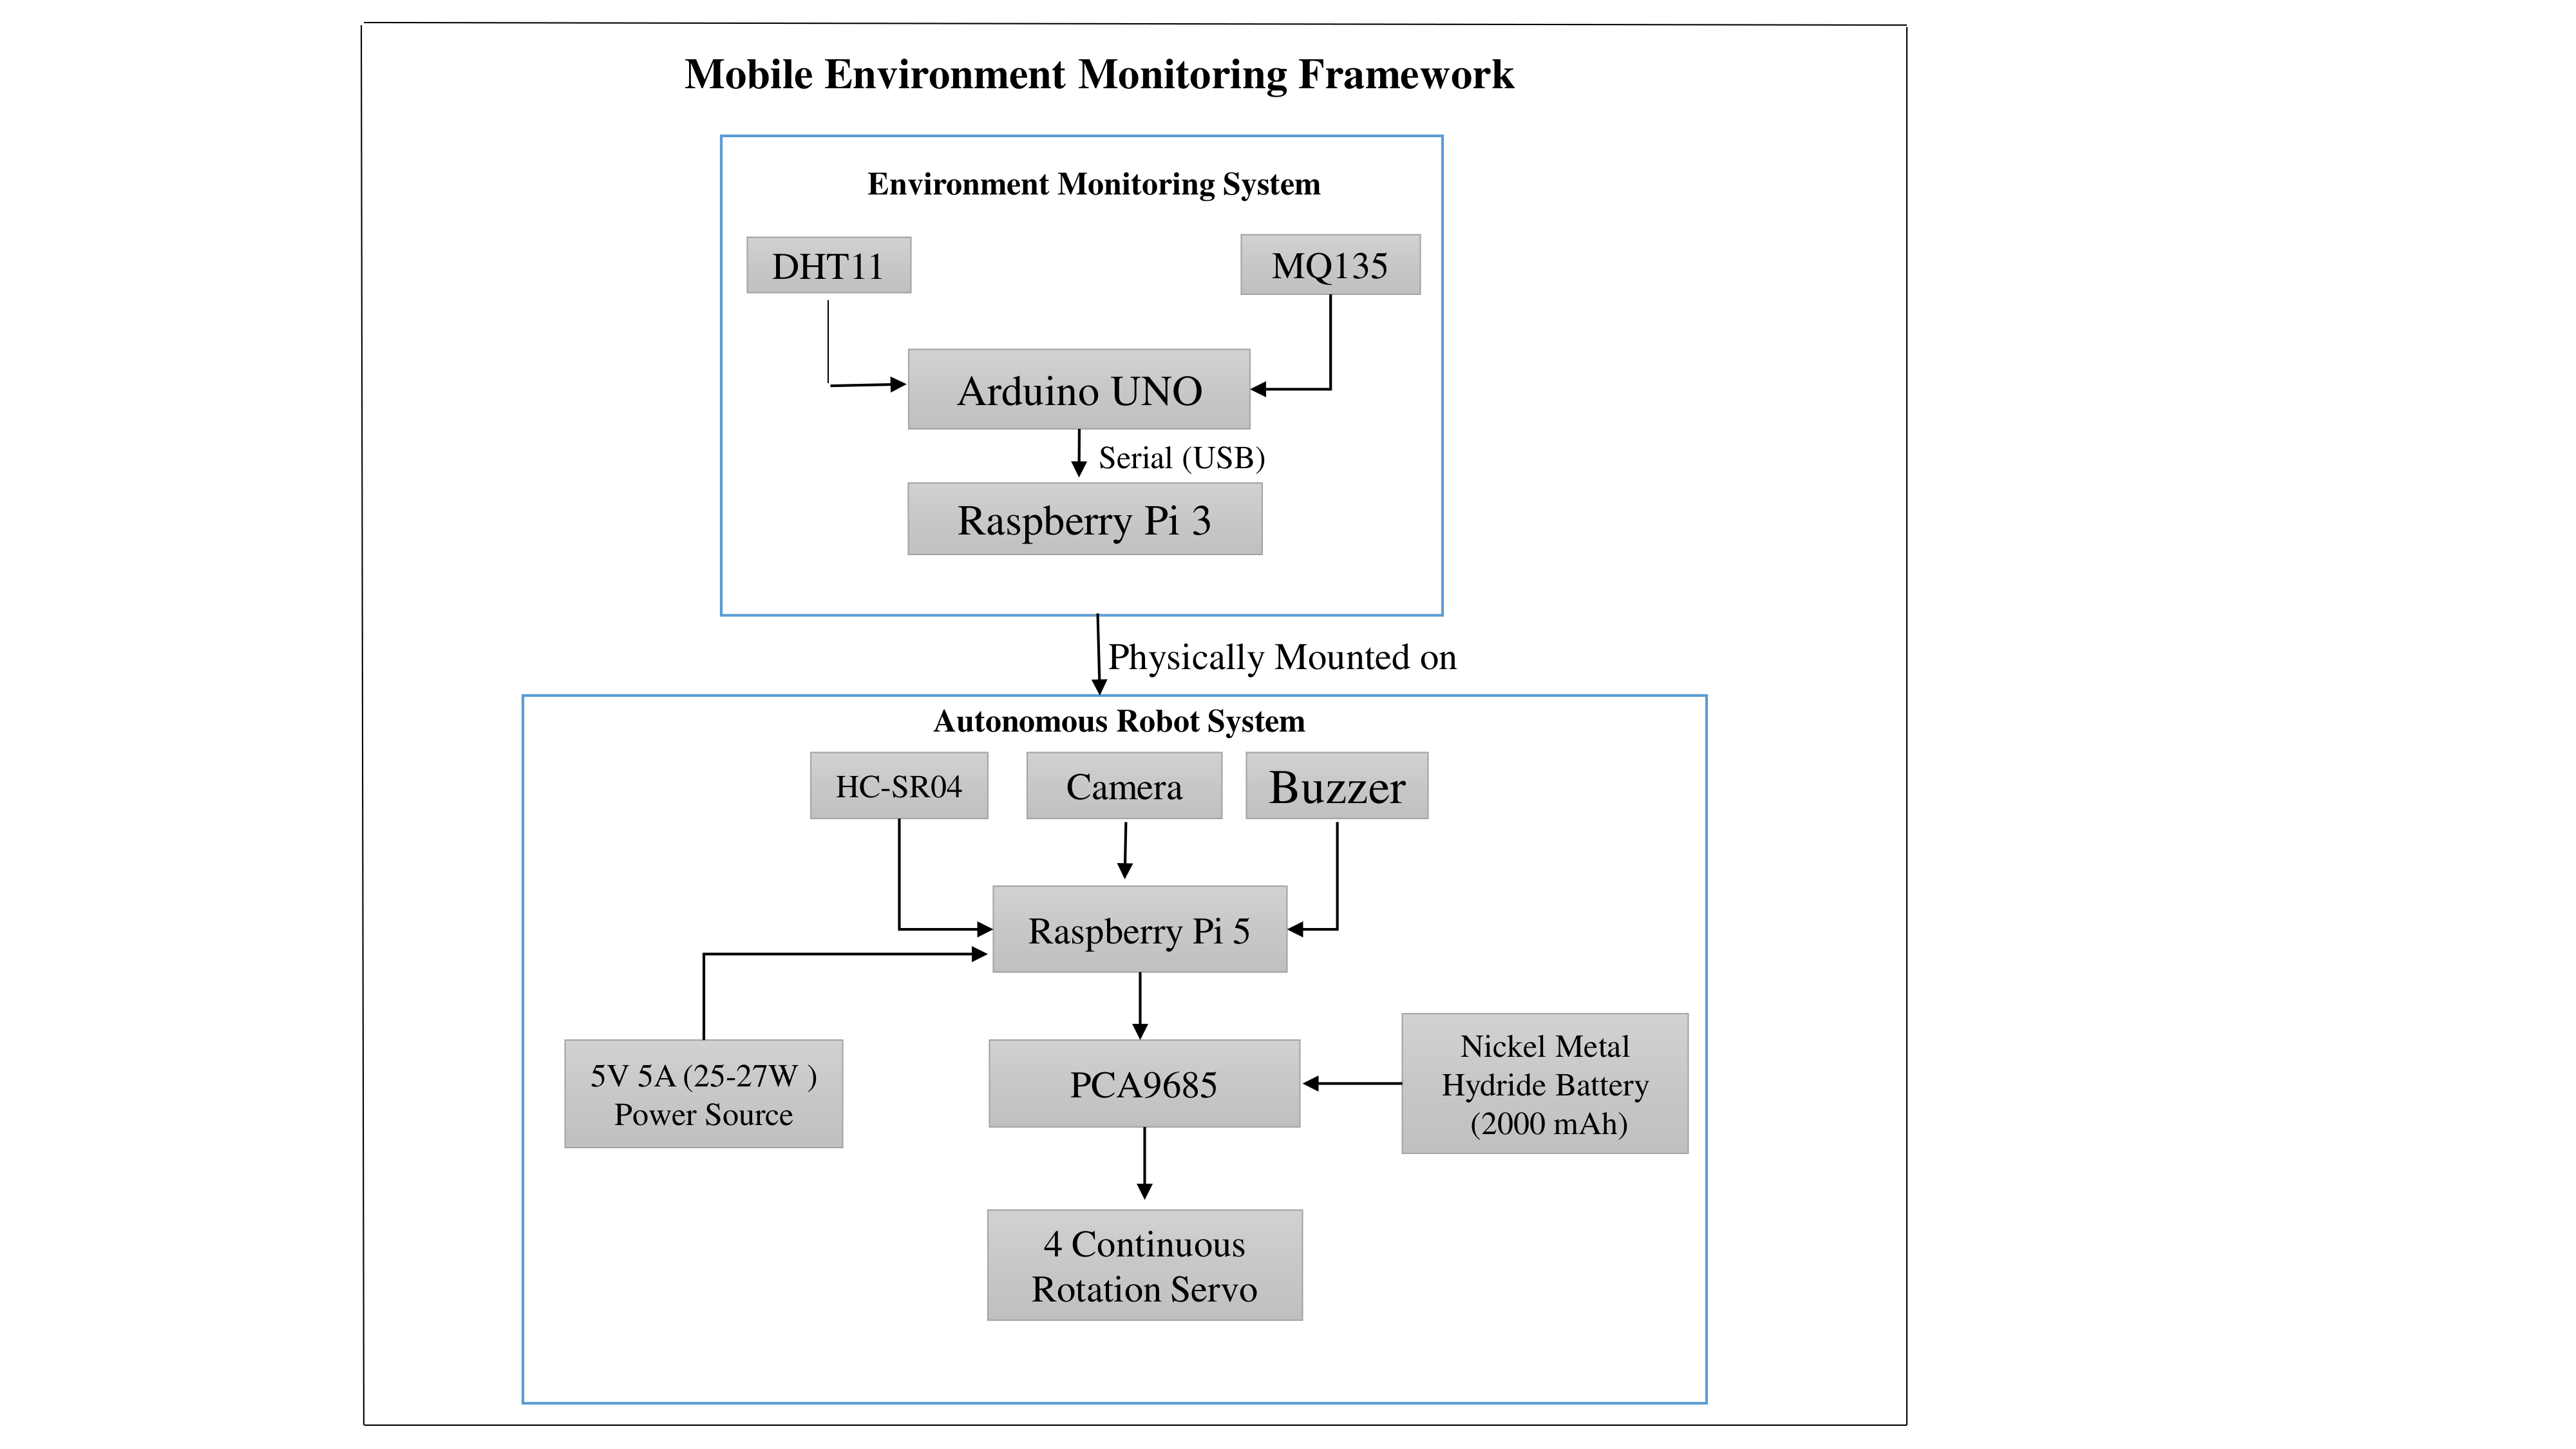
\includegraphics[width=1.4\textwidth]{system_architecture.png}%
  }
  \caption{Overall system architecture of the proposed framework.}
  \label{fig:sysarch}
\end{figure}

\section{Hardware Design and Manual Robot Construction}

The mobile platform constitutes the physical foundation of the
framework. A four-wheel differential-drive chassis was selected for
its mechanical simplicity, ease of control, and established suitability
for structured indoor navigation tasks \cite{r10,r11}. This choice
is consistent with the majority of experimental mobile robot platforms
reported in the literature \cite{r9,r18}.

\subsection{Mechanical Platform and Drive System}

Four continuous-rotation servo motors serve as drive actuators, mounted
on a rigid aluminium chassis with two motors per side. The servo motors
are controlled through a PCA9685 16-channel PWM driver
operating at 50\,Hz over the I$^2$C bus of the Raspberry Pi~5 \cite{r38}.
The PCA9685 generates pulse-width modulated signals in the range
1000--2000\,$\mu$s, where a centre pulse of 1600\,$\mu$s corresponds
to the stationary state, values above 1600\,$\mu$s command forward
rotation, and values below 1600\,$\mu$s command reverse rotation.
Individual calibration factors are applied to each motor channel to
compensate for mechanical asymmetries arising from servo manufacturing
tolerances.

Table~\ref{tab:motor} lists the four motor channels with their
respective chassis positions, rotation directions, and calibration
factors. Channel 0 drives the rear right motor in the normal direction
with a calibration factor of 1.335, while channel 1 drives the rear
left motor in the reversed direction with a factor of 0.790. Channel 2
drives the front right motor in the normal direction and requires the
highest calibration factor of 2.335, and channel 3 drives the front
left motor in the reversed direction with a factor of 0.290. These
asymmetric factors reflect the physical differences between the four
servo units and were determined empirically to achieve straight-line
motion on a flat surface.

\begin{table}[tbp]
  \centering
  \caption{Motor channel assignments and calibration factors.}
  \label{tab:motor}
  \begin{tabular}{cccc}
    \toprule
    Channel & Position    & Direction & Calibration Factor \\
    \midrule
    0       & Rear Right  & Normal    & 1.335 \\
    1       & Rear Left   & Reversed  & 0.790 \\
    2       & Front Right & Normal    & 2.335 \\
    3       & Front Left  & Reversed  & 0.290 \\
    \bottomrule
  \end{tabular}
\end{table}

\subsection{Sensing and Perception Hardware}

The following sensors and peripheral devices are integrated onto the
robot platform.

The HC-SR04 ultrasonic sensor is mounted at the front lower
section of the chassis, connected to GPIO pin 23 (TRIG) and GPIO pin
24 (ECHO) of the Raspberry Pi~5 \cite{r34}. The sensor emits 40\,kHz
ultrasonic pulses and computes obstacle distance from the echo return
time. Any measurement below 20\,cm triggers automatic forward-motion
blocking and activates the buzzer alert.

The Logitech Brio 100 USB Camera is mounted centrally on a
forward-facing bracket above the chassis at a height of 20\,cm above
the floor surface, angled 45$^\circ$ downward toward the path. The
camera captures frames at a resolution of 640$\times$480 pixels at 30
frames per second through the device node \texttt{/dev/video0}. This
mounting configuration ensures that the path tape is fully within the
camera field of view at the operating height.

The active buzzer is connected to GPIO pin 18 and is activated
by the obstacle detection thread whenever an object is detected within
the 20\,cm safety threshold.

The power supply consists of a dedicated 5\,V, 5\,A
(25--27\,W) regulated unit powering the Raspberry Pi~5 and the PCA9685
driver, and a separate 2000\,mAh Nickel Metal Hydride battery pack
powering the four servo motors. This separation isolates motor current
transients from the logic supply rail, preventing voltage fluctuations
from disrupting the Raspberry Pi~5 during rapid motor direction changes.

Figure~\ref{fig:robot} shows the fully assembled robot platform. The
Logitech Brio 100 camera is visible at the top centre of the chassis
body. The HC-SR04 ultrasonic sensor is mounted at the front lower
section facing forward.

\begin{figure}[tbp]
  \centering
  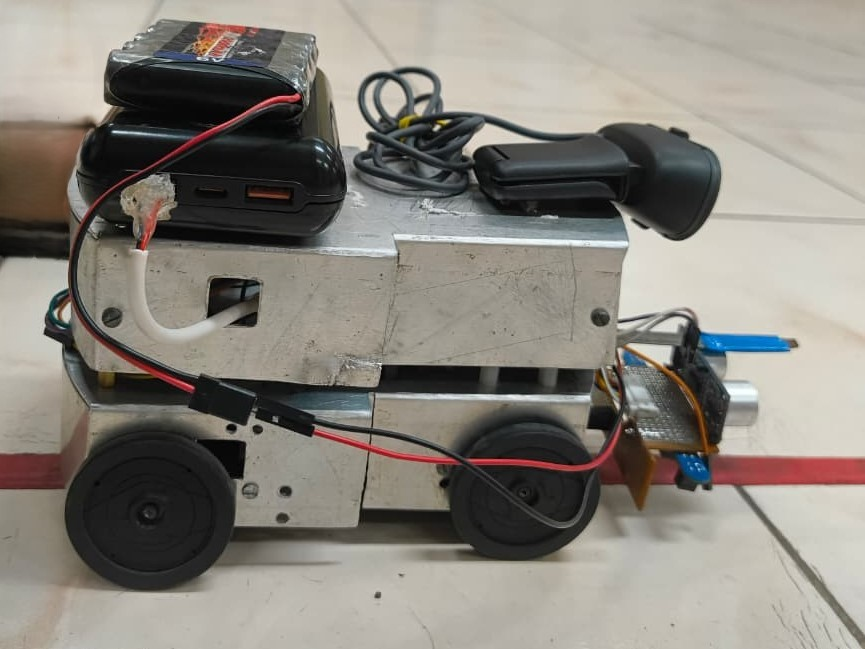
\includegraphics[width=0.85\textwidth]{WhatsApp Image 2026-04-10 at 1.09.05 PM (2).jpeg}
  \caption{Assembled mobile robot platform showing the Logitech Brio~100
  camera mounted at the top centre, the HC-SR04 ultrasonic sensor at
  the front lower section.}
  \label{fig:robot}
\end{figure}

\subsection{Web-Based Manual Control System}

Prior to the deployment of autonomous navigation software, a
web-based teleoperation interface was implemented to verify motor
functionality, sensor integration, and hardware communication under
manual human supervision \cite{r2}. The backend is implemented as a
Flask RESTful application \cite{r37} exposing dedicated API endpoints
for directional commands (forward, backward, left, right, and stop)
and variable speed control. A responsive HTML, CSS, and JavaScript
dashboard is served at \texttt{http://<Pi-IP>:5000} and is accessible
from any device connected to the same local network. The interface
supports button-based, touch-based, and keyboard-based controls using
the W/A/S/D key set and directional arrow keys. A multi-threaded
software architecture ensures that the motor command thread, obstacle
monitoring thread, and Flask HTTP serving thread execute concurrently
without blocking one another. This phase validated mechanical
operability and sensor responsiveness before the autonomous control
stack was deployed.

\section{Path Dataset Collection and YOLOv8 Model Training}

\subsection{Path Design and Data Collection}

A navigable path was constructed using red adhesive tape laid
on tiled and concrete floor surfaces within the laboratory environment
at the Central Scientific and Industrial Research -- Central Mechanical
Engineering Research Institute. Red tape was selected because it provides
high colour contrast against typical indoor floor colours under both
natural daylight and artificial fluorescent lighting conditions. The
Logitech Brio 100 camera was mounted at 20\,cm above the floor surface
and angled 45$^\circ$ downward, capturing images at a resolution of
640$\times$480 pixels. A total of 289 images were collected, covering
three path geometry categories: straight sections at 40\%, curved
sections at 35\%, and complex turns with direction changes at 25\%.
Lighting conditions were varied to include well-lit (60\%), low-light
(25\%), and mixed shadow (15\%) scenarios, ensuring dataset diversity
for robust model generalisation \cite{r32,r31}.

\subsection{Image Annotation and Dataset Preparation}

Each of the 289 captured images was annotated using the
Computer Vision Annotation Tool (CVAT) platform \cite{r31}.
Polygon annotations were drawn manually around the navigable path
region in each image frame, labelling the path foreground as class
\texttt{path} (class index 0). The annotations were exported in YOLO
segmentation format and validated through visual inspection. Ambiguous
or low-quality samples were removed during the inspection pass. The
dataset was then partitioned into three splits using a 70/20/10 ratio.

Table~\ref{tab:split} presents the resulting split distribution. The
training split contains 202 images and 202 corresponding label files.
The validation split contains 57 images and labels, and the test split
contains 30 images and labels.

\begin{table}[tbp]
  \centering
  \caption{Dataset split distribution.}
  \label{tab:split}
  \begin{tabular}{ccc}
    \toprule
    Split      & Images & Labels \\
    \midrule
    Training   & 202    & 202 \\
    Validation & 57     & 57 \\
    Test       & 30     & 30 \\
    \midrule
    Total      & 289    & 289 \\
    \bottomrule
  \end{tabular}
\end{table}

\subsection{Model Architecture}

The YOLOv8n-seg (nano segmentation) variant of the YOLOv8
architecture was selected as the segmentation model \cite{r32}.
The model contains 86 fused layers with 3,258,259 parameters,
zero gradients in inference mode, and a computational cost of
11.3~GFLOPs.

The YOLOv8 family provides five model scale variants ---
nano~(n), small~(s), medium~(m), large~(l), and extra-large~(x)
--- each progressively increasing in parameter count, computational
cost, and reported accuracy on standard benchmarks \cite{r32}.
Table~\ref{tab:yolov8compare} presents a comparison of the five
variants on the COCO dataset alongside their approximate CPU inference
performance on an embedded single-board computer.

\begin{table}[tbp]
  \centering
  \caption{YOLOv8 segmentation variant comparison (COCO val2017) \cite{r32}.}
  \label{tab:yolov8compare}
  \begin{tabular}{lcccc}
    \toprule
    Variant        & Params (M) & GFLOPs & Mask mAP@50-95 & CPU Latency \\
    \midrule
    YOLOv8n-seg    & 3.4        & 12.6   & 36.7           & $\sim$65\,ms \\
    YOLOv8s-seg    & 11.8       & 42.6   & 42.6           & $\sim$190\,ms \\
    YOLOv8m-seg    & 27.3       & 110.2  & 49.9           & $\sim$440\,ms \\
    YOLOv8l-seg    & 46.0       & 220.5  & 52.3           & $\sim$870\,ms \\
    YOLOv8x-seg    & 71.8       & 344.1  & 53.4           & $>$1200\,ms  \\
    \bottomrule
    \multicolumn{5}{l}{\small CPU latency measured on a Raspberry Pi~5 at 320$\times$320 resolution.}
  \end{tabular}
\end{table}

As Table~\ref{tab:yolov8compare} shows, the larger variants (YOLOv8s
through YOLOv8x) achieve higher mask mAP@50-95 values on the
general COCO benchmark, ranging from 42.6 to 53.4. However, their
CPU latencies on the Raspberry Pi~5 at 320$\times$320 resolution
range from approximately 190\,ms to over 1200\,ms, corresponding to
frame rates of 5.3\,FPS down to below 1\,FPS. None of these variants
can sustain the minimum 15\,FPS required for stable closed-loop PID
control on the Raspberry Pi~5 CPU \cite{r34,r29}. The nano variant,
by contrast, achieves 15.4\,FPS after ONNX conversion, as demonstrated
in the benchmarking results in Section~\ref{sec:opt}, and this is the
only variant that clears the real-time threshold on the available
embedded hardware.

The task addressed in this work is fundamentally simpler than the
general COCO benchmark: the model is required to segment a single
highly distinctive class (red adhesive tape) under controlled
indoor lighting against a uniform tiled background. In this specific
setting, a high generalisation capacity is not required and the
performance gap between nano and larger variants is expected to
narrow substantially with fine-tuning \cite{r30,r32}. The trained
YOLOv8n-seg model achieved a mask mAP@50 of 0.988 on the
57-image validation split, which exceeds the mAP@50 values reported
for the larger variants on COCO, confirming that for this task
the nano variant provides accuracy that is more than sufficient.

The nano variant was therefore selected on the following grounds:

\begin{itemize}
  \item Only the nano variant meets the real-time constraint of
        15\,FPS on the Raspberry Pi~5 CPU after ONNX conversion.
  \item The task involves segmenting a single, visually distinctive
        class, which does not require the generalisation capacity
        of larger models.
  \item The fine-tuned model achieves 0.988 mask mAP@50, which is
        sufficient for reliable closed-loop path following.
  \item The lower parameter count (3.4~M) reduces memory footprint
        to 280\,MB at 320$\times$320, within the operational limit
        of the 4\,GB Raspberry Pi~5 \cite{r34}.
\end{itemize}

The model accepts a single class label (\texttt{path}) and produces
instance segmentation masks together with bounding boxes at each
inference step \cite{r12,r13,r29}.

\subsection{Training Configuration and Procedure}

Training was performed on Google Colab using a Tesla T4 GPU (15095\,MB
VRAM) with the Ultralytics 8.4.7 framework \cite{r32} under PyTorch
2.9.0 with CUDA 12.6.

Table~\ref{tab:training} presents the complete training configuration.
Training ran for a maximum of 200 epochs with an early stopping patience
of 30 epochs, meaning training was terminated if the validation mAP did
not improve for 30 consecutive epochs. A batch size of 8 was used with
the Adam optimizer and an initial and final learning rate of 0.01. The
model was initialised from the official pretrained \texttt{yolov8n-seg.pt}
weights and fine-tuned on the custom path dataset. Mixed-precision
automatic mixed precision (AMP) training was enabled. Data augmentation
included mosaic augmentation at probability 1.0, horizontal flip at
0.5, HSV hue, saturation and value shifts, translation of 0.1, and
scale variation of 0.5. The warmup phase ran for 3 epochs.

\begin{table}[tbp]
  \centering
  \caption{YOLOv8n-seg training configuration.}
  \label{tab:training}
  \begin{tabular}{ll}
    \toprule
    Parameter               & Value \\
    \midrule
    Epochs                  & 200 \\
    Early stopping patience & 30 epochs \\
    Batch size              & 8 \\
    Input resolution        & 640$\times$640 \\
    Optimizer               & Adam \\
    Initial learning rate   & 0.01 \\
    Final learning rate     & 0.01 \\
    Momentum                & 0.937 \\
    Weight decay            & 0.0005 \\
    Warmup epochs           & 3 \\
    Mosaic augmentation     & 1.0 \\
    Horizontal flip         & 0.5 \\
    HSV-Hue                 & 0.015 \\
    HSV-Saturation          & 0.7 \\
    HSV-Value               & 0.4 \\
    Translation             & 0.1 \\
    Scale                   & 0.5 \\
    Pretrained weights      & yolov8n-seg.pt \\
    Mixed precision (AMP)   & Enabled \\
    \bottomrule
  \end{tabular}
\end{table}

\subsection{Validation Results}

The trained model was evaluated on the 57-image validation split
immediately after training. Table~\ref{tab:val} presents the validation
metrics across both the bounding box detection task and the instance
segmentation mask task. For the bounding box task, the model achieved a
precision of 0.947, a recall of 0.946, an mAP@50 of 0.973, and an
mAP@50-95 of 0.821. For the segmentation mask task, precision was 0.965,
recall was 0.963, mAP@50 was 0.988, and mAP@50-95 was 0.736. The mask
mAP@50 of 0.988 indicates that the model reliably segments the red tape
path in 96 out of every 100 validation frames at the standard IoU
threshold. The best checkpoint was saved to \texttt{best.pt} based on
the highest validation mAP@50.

\begin{table}[tbp]
  \centering
  \caption{YOLOv8n-seg validation metrics on the 57-image validation split.}
  \label{tab:val}
  \begin{tabular}{lcccc}
    \toprule
    Task  & Precision & Recall & mAP@50 & mAP@50-95 \\
    \midrule
    Box   & 0.947     & 0.946  & 0.973  & 0.821 \\
    Mask  & 0.965     & 0.963  & 0.988  & 0.736 \\
    \bottomrule
  \end{tabular}
\end{table}

\subsection{Model Optimisation for Embedded Deployment}
\label{sec:opt}

Direct deployment of the trained PyTorch \texttt{best.pt} model on the
Raspberry Pi~5 CPU at 640$\times$640 resolution produced an average
inference time of 101.6\,ms, corresponding to 9.8 frames per second.
This throughput is insufficient for stable closed-loop control, which
requires a sustained minimum of 10 to 15 frames per second
\cite{r29,r10}. A two-stage optimisation pipeline was applied to meet
this requirement.

\paragraph{Stage 1: Resolution Tuning.}
Inference resolution was benchmarked at three settings on the
Raspberry Pi~5 (Broadcom BCM2712, quad-core Cortex-A76 at 2.4\,GHz,
4\,GB LPDDR4X RAM, ONNX Runtime 1.23.2) using 20 inference iterations
per configuration. As shown in Table~\ref{tab:bench}, at 640$\times$640
resolution, inference takes 101.6\,ms on average, yielding 9.8\,FPS
with a memory footprint of 450\,MB. Reducing resolution to
480$\times$480 increases the average inference time to 201.3\,ms,
reducing throughput to 5.0\,FPS. At 320$\times$320, inference time
is 103.0\,ms, yielding 9.7\,FPS with a reduced memory footprint of
280\,MB.

\begin{table}[tbp]
  \centering
  \caption{Resolution benchmarking on Raspberry Pi~5 in PyTorch format.}
  \label{tab:bench}
  \begin{tabular}{cccc}
    \toprule
    Resolution       & Average Inference Time & FPS & Memory Usage \\
    \midrule
    640$\times$640   & 101.6\,ms              & 9.8 & 450\,MB \\
    480$\times$480   & 201.3\,ms              & 5.0 & 350\,MB \\
    320$\times$320   & 103.0\,ms              & 9.7 & 280\,MB \\
    \bottomrule
  \end{tabular}
\end{table}

\paragraph{Stage 2: ONNX Conversion.}
The best checkpoint was exported from PyTorch to ONNX format at a
fixed static input shape of 320$\times$320 using the Ultralytics ONNX
export pipeline \cite{r33}. Inference was executed using ONNX Runtime
with \texttt{CPUExecutionProvider}. As shown in Table~\ref{tab:onnx},
the ONNX model reduces average inference time from 103.0\,ms to
64.8\,ms, increasing throughput from 9.7\,FPS to 15.4\,FPS,
representing a speedup factor of 1.57$\times$ over the PyTorch baseline.

\begin{table}[tbp]
  \centering
  \caption{PyTorch versus ONNX inference comparison at 320$\times$320.}
  \label{tab:onnx}
  \begin{tabular}{ccccc}
    \toprule
    Format  & Resolution     & Average Time & FPS  & Speedup \\
    \midrule
    PyTorch & 320$\times$320 & 103.0\,ms    & 9.7  & 1.0$\times$ \\
    ONNX    & 320$\times$320 & 64.8\,ms     & 15.4 & 1.57$\times$ \\
    \bottomrule
  \end{tabular}
\end{table}

The FPS progression across all four model configurations is illustrated
in Figure~\ref{fig:tradeoff}, which plots FPS on the vertical axis
against four model configurations: 640 PyTorch, 480 PyTorch, 320
PyTorch, and 320 ONNX. The figure confirms that ONNX conversion at
320$\times$320 resolution is the only configuration that meets the
real-time threshold of 15 FPS, making format conversion the decisive
optimisation step.

\begin{figure}[tbp]
  \centering
  \includegraphics[width=0.88\textwidth]{accuracy_speed_tradeoff.png}
  \caption{FPS comparison across all four model configurations
  (640 PyTorch, 480 PyTorch, 320 PyTorch, 320 ONNX) on the
  Raspberry Pi~5 CPU, confirming that ONNX at 320$\times$320 is the
  only configuration meeting the 15\,FPS real-time threshold.}
  \label{fig:tradeoff}
\end{figure}

A 30-minute continuous stability test confirmed an average throughput
of $15.2 \pm 0.8$ FPS, a peak of 16.8 FPS, a minimum of 13.9 FPS,
zero memory leaks, and a CPU temperature stable at $68 \pm 2\,^\circ$C
without thermal throttling. The optimised model was saved as
\texttt{best\_320.onnx} and deployed to the \texttt{models/} directory
on the Raspberry Pi~5.

\section{Autonomous Path-Following System}

\subsection{Control Flow Overview}

The control flow of the complete autonomous path-following system is
illustrated in Figure~\ref{fig:robotflow}. The flowchart describes the
sequential and conditional logic that governs robot behaviour from
startup to shutdown.

The following steps describe the sequential and conditional logic
executed by the robot during each autonomous cycle:

\begin{enumerate}

  \item \emph{Start.} The system begins execution when the operator
        issues a START command through the web dashboard.

  \item \emph{Initialise camera, motors, and sensors.} The Raspberry
        Pi~5 opens the camera stream at 640$\times$480 resolution,
        initialises the I$^2$C connection to the PCA9685, and confirms
        GPIO pin assignments for the HC-SR04 and buzzer.

  \item \emph{Capture frame from camera.} At each iteration of the
        vision loop running at 20\,Hz, a single frame is captured from
        the camera buffer.

  \item \emph{Run YOLO segmentation.} The captured frame is resized
        to 320$\times$320 pixels and passed to the ONNX Runtime session.
        The model produces an instance segmentation mask for the
        \texttt{path} class and a confidence score.

  \item \emph{Is path detected?} The YOLO output is checked for valid
        detections within the region of interest (bottom 30\% of frame).
        If no detection is present, the robot is stopped and the vision
        loop returns to step~3 to attempt path reacquisition.

  \item \emph{Calculate centroid.} If a valid path detection is present,
        the centroid of the segmentation mask within the ROI is computed,
        representing the horizontal centre of the detected path.

  \item \emph{Compute error (deviation).} The horizontal centroid
        position is compared to the horizontal centre of the camera
        frame. The difference is normalised to the range
        $[-1.0,\,+1.0]$ and constitutes the path deviation error
        signal $e(t)$.

  \item \emph{Apply deadband.} A deadband filter of $\pm 0.04$ is
        applied to the deviation signal to prevent the PID controller
        from generating unnecessary steering corrections on
        near-straight sections.

  \item \emph{Read ultrasonic sensor.} The HC-SR04 sensor is triggered
        and the echo pulse duration is converted to distance in
        centimetres.

  \item \emph{Is obstacle detected?} The measured distance is compared
        to the 20\,cm safety threshold. If an obstacle is present,
        all motor channels are set to neutral and the buzzer is
        activated.

  \item \emph{Apply PID control.} If no obstacle is detected, the
        deadband-filtered error $e(t)$ is processed by the PID
        controller using Equation~\eqref{eq:pid} with gains
        $K_p = 13.2$, $K_i = 0.0$, and $K_d = 0.475$.

  \item \emph{Send signal to motor driver.} The steering correction
        $u(t)$ from Equation~\eqref{eq:pid} is combined with the base
        forward speed. Per-wheel calibration factors from
        Table~\ref{tab:motor} are applied before writing pulse widths
        to the PCA9685 over I$^2$C.

  \item \emph{Move robot.} The PCA9685 outputs the computed PWM signals
        to the four servo motors.

  \item \emph{Is stopped by the user?} After each control cycle, the
        system checks for a STOP command. If received, the loop
        terminates and all motors are set to neutral; otherwise the flow
        returns to step~3.

\end{enumerate}

\begin{figure}[p]
  \centering
  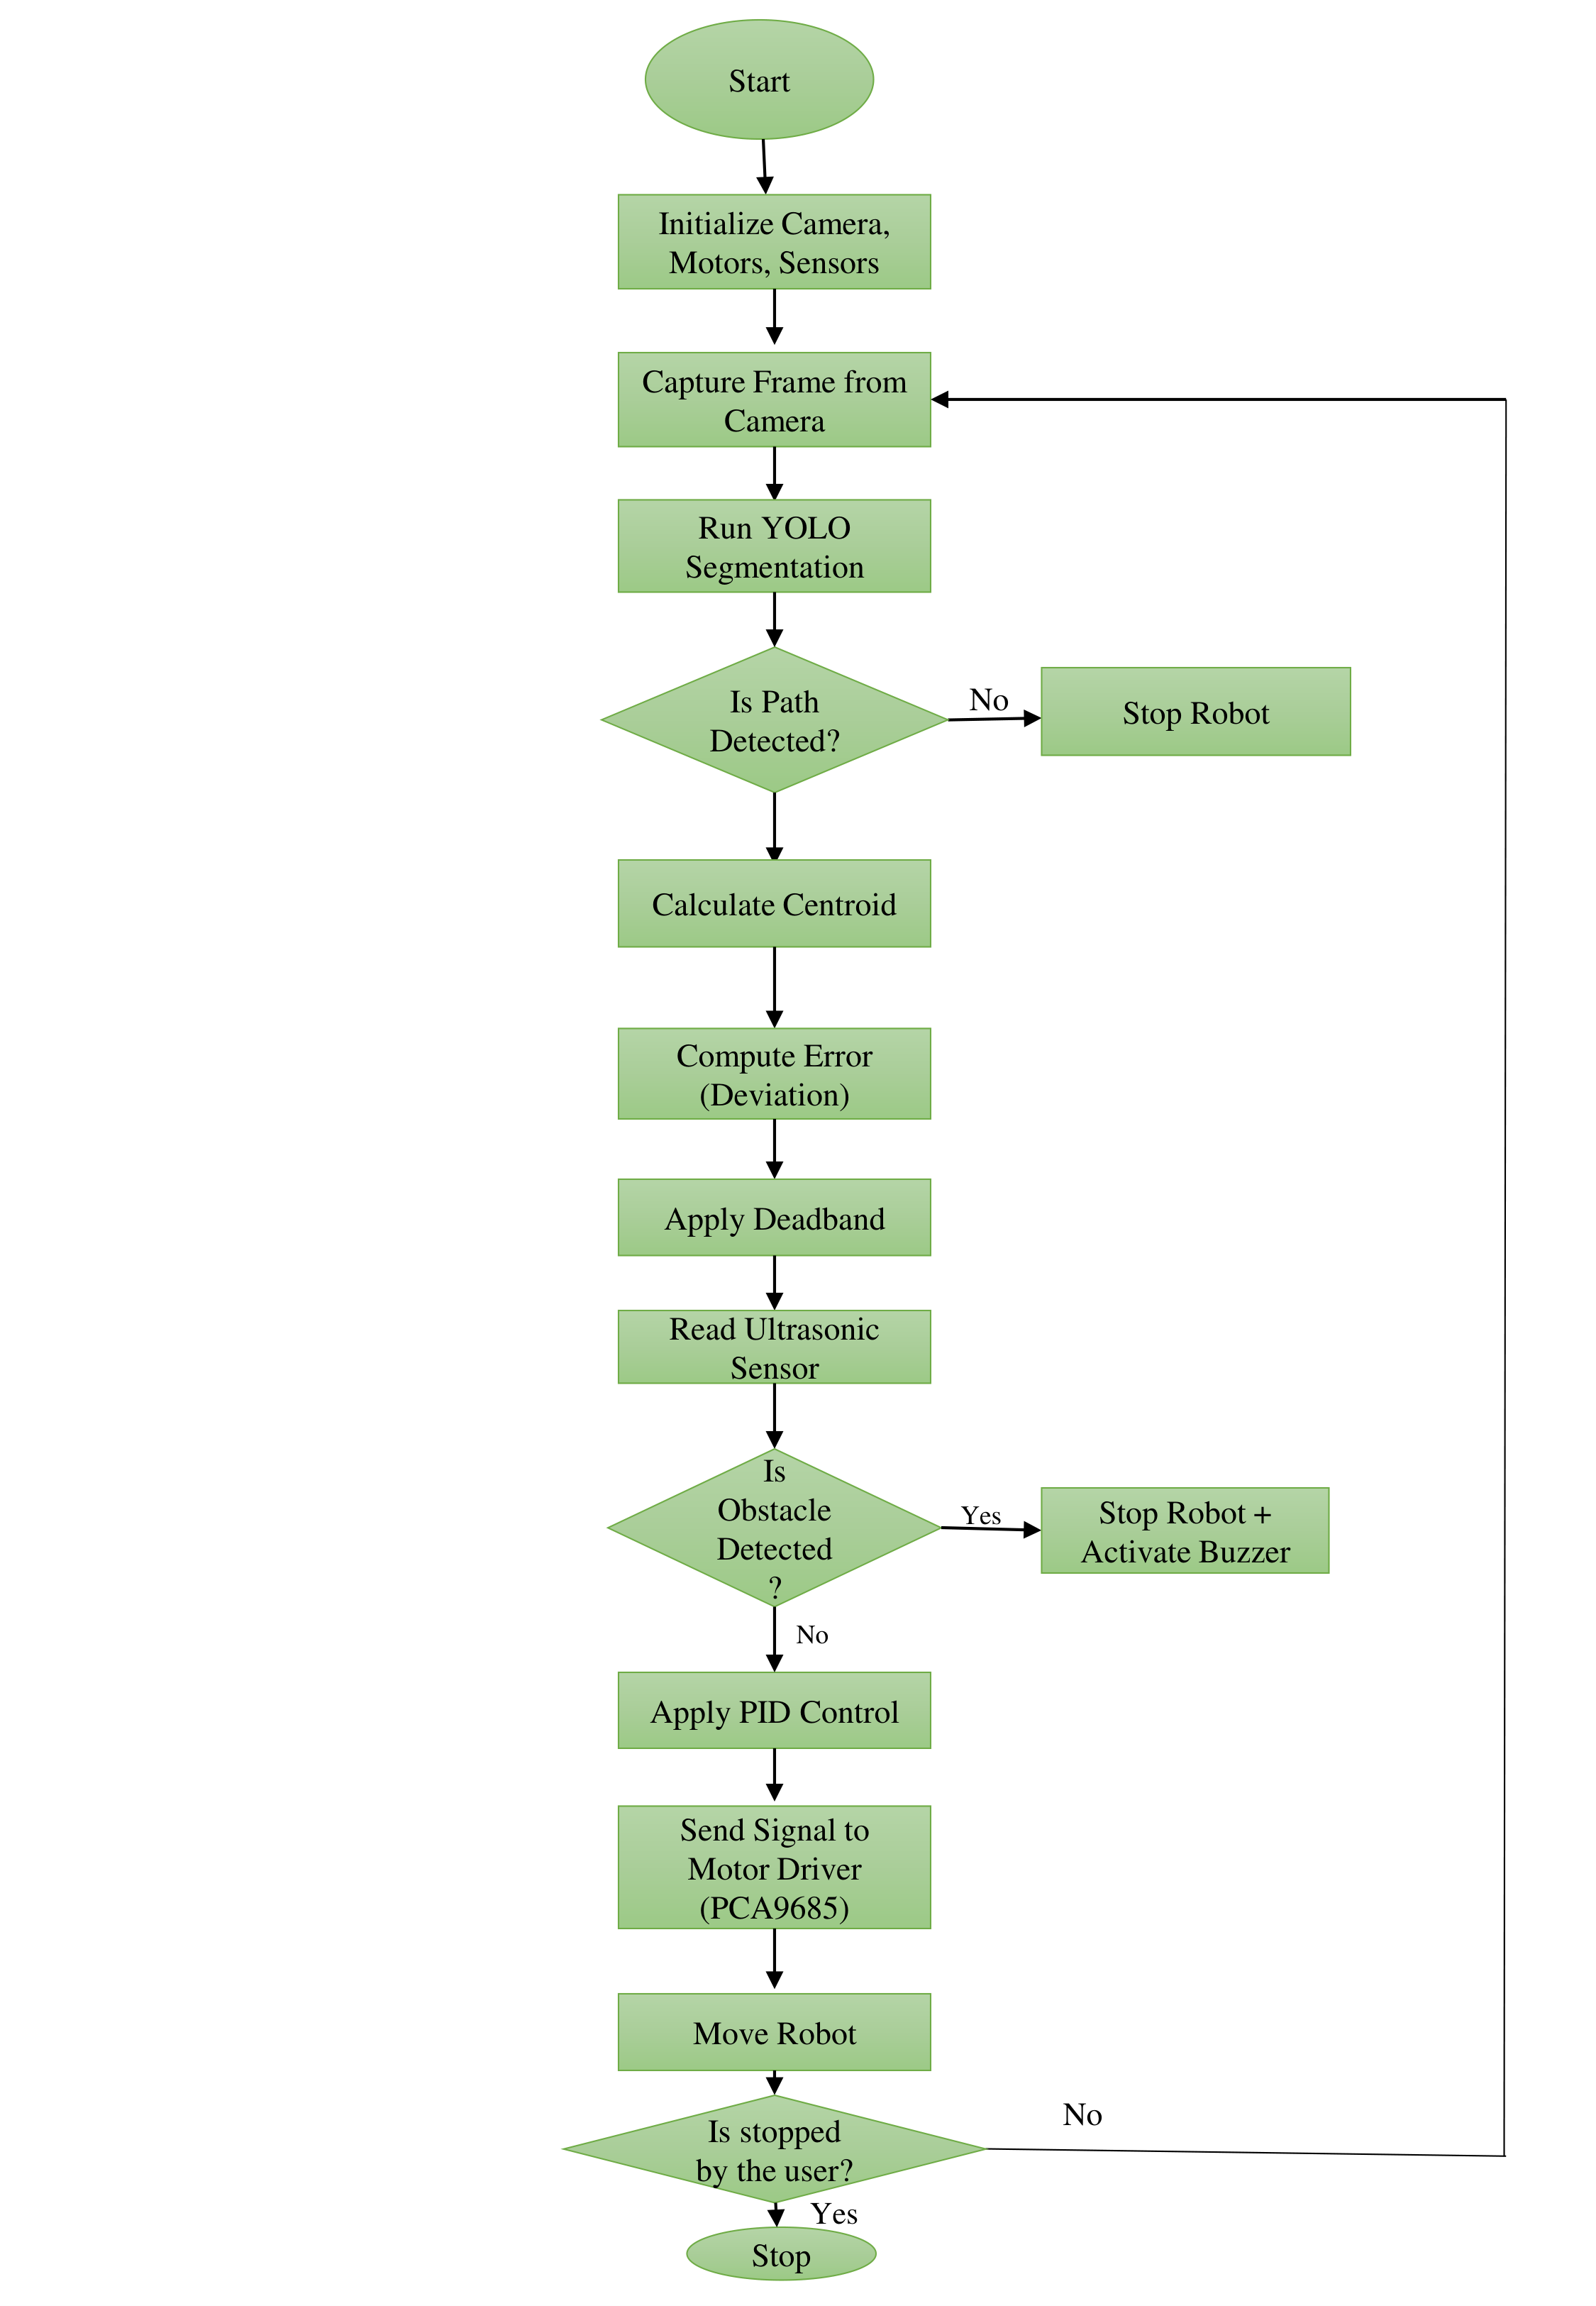
\includegraphics[height=0.88\textheight]{robot_flowchart.png}
  \caption{Step-by-step control flow of the autonomous path-following robot.}
  \label{fig:robotflow}
\end{figure}

\clearpage

\subsection{Threading Architecture}

The autonomous navigation software is structured around a four-thread
concurrent execution model \cite{r26}. Table~\ref{tab:threads}
summarises the four threads and their responsibilities.

\begin{table}[tbp]
  \centering
  \caption{Concurrent thread model of the autonomous navigation system.}
  \label{tab:threads}
  \begin{tabular}{lcc}
    \toprule
    Thread Name                          & Rate    & Responsibility \\
    \midrule
    \texttt{\_vision\_loop}              & 20\,Hz  & ONNX inference, PID control, CSV logging \\
    \texttt{\_obstacle\_detection\_loop} & 10\,Hz  & HC-SR04 polling, buzzer activation \\
    \texttt{\_movement\_loop}            & 10\,Hz  & PWM motor command execution \\
    \texttt{\_encoder\_loop}             & 100\,Hz & Speed ramp simulation \\
    \bottomrule
  \end{tabular}
\end{table}

\subsection{Vision Module and Real-Time Path Segmentation}

At each cycle of the vision loop, a 640$\times$480 pixel frame is
captured from the camera and passed to the ONNX Runtime inference
session at the fixed input resolution of 320$\times$320 pixels. The
YOLOv8n-seg model produces instance segmentation masks for the class
\texttt{path} within the bottom 30\% ROI.

Figure~\ref{fig:detect} illustrates the real-time path segmentation
output during an autonomous run. The green overlay represents the
YOLOv8 instance segmentation mask for the \texttt{path} class. The
output is produced in real time at 15.4\,FPS on the Raspberry Pi~5 CPU.

\begin{figure}[tbp]
  \centering
  \includegraphics[width=0.88\textwidth]{capture_1.jpg}
  \caption{Real-time YOLOv8n-seg path segmentation output at 15.4\,FPS on the Raspberry Pi~5 CPU. The green mask overlay covers the detected \texttt{path} class within the bottom 30\% ROI; the deviation arrow indicates the current PID steering correction direction and magnitude.}
  \label{fig:detect}
\end{figure}

During an autonomous run, the bottom 30\% region of interest is
highlighted with the YOLOv8 segmentation mask drawn in green over the
detected red-tape path. The path centroid is marked, and the deviation
arrow indicates the direction and magnitude of the current steering
correction. This overlay was visible in the live MJPEG feed on the web
dashboard throughout all 20 autonomous trials.

Within the ROI, the horizontal centroid of the detected path mask is
computed and normalised relative to the horizontal frame centre to
produce a deviation signal in the range $[-1.0,\,+1.0]$. A deadband
filter of $\pm 0.04$ is applied before the signal is passed to the
PID controller.

Algorithm~\ref{alg:vision} formalises the complete vision-based deviation computation executed at every cycle of the \texttt{\_vision\_loop} thread at 20\,Hz. The procedure begins by resizing the captured frame to $320\times320$ pixels, which matches the fixed static input shape of the deployed ONNX model. The ONNX Runtime session is then called to produce a set of instance segmentation masks $\mathcal{M}$ and their corresponding confidence scores $\mathcal{S}$. If no detection is returned, or if the highest confidence score falls below the threshold of 0.50, the function returns \texttt{None}, signalling the main loop to halt forward motion and await path reacquisition. When a valid detection is present, the mask with the highest confidence score is selected and cropped to the bottom 30\% region of interest. The centroid of the binary mask within that region is computed as a pixel-weighted mean, yielding the horizontal position $C_x$. This position is normalised to the range $[-1.0,\,+1.0]$ relative to the frame half-width, and a deadband of $\pm 0.04$ is applied to suppress spurious corrections on near-straight sections. The resulting scalar $d$ is the deviation signal consumed by the PID steering controller.

\begin{algorithm}[H]
\DontPrintSemicolon
\caption{Vision-Based Path Deviation Computation}
\label{alg:vision}
\KwIn{Camera frame $F$ at $640\times480$ resolution}
\KwOut{Normalised lateral deviation $d\in[-1.0,\,+1.0]$, or \texttt{None} if no path found}
\BlankLine
Resize $F$ to $320\times320$ pixels for ONNX Runtime input\;
$\mathcal{M},\,\mathcal{S} \leftarrow \texttt{ONNX.run}(F)$ \tcp*{instance masks and confidence scores}
\If{$|\mathcal{S}|=0$ \textbf{or} $\max(\mathcal{S})<0.50$}{
  \Return \texttt{None} \tcp*{no path detected above threshold}
}
Select best mask $M^{*} \leftarrow \mathcal{M}[\arg\max(\mathcal{S})]$\;
Define ROI as bottom 30\% of frame: rows $\lfloor 0.70H\rfloor$ to $H$\;
$M_{\text{roi}} \leftarrow M^{*}\cap\text{ROI}$\;
\If{$\sum M_{\text{roi}}=0$}{
  \Return \texttt{None} \tcp*{mask absent from ROI}
}
Compute centroid: $\displaystyle C_x = \frac{\sum_{i,j} j\cdot M_{\text{roi}}[i,j]}{\sum_{i,j} M_{\text{roi}}[i,j]}$\;
Normalise: $d \leftarrow \dfrac{C_x - W/2}{W/2}$, where $W=640$\;
Apply deadband: \textbf{if} $|d|<0.04$ \textbf{then} $d\leftarrow 0.0$\;
\Return $d$\;
\end{algorithm}

\subsection{PID Steering Controller}

The path deviation signal after deadband filtering serves as the error
input $e(t)$ to a discrete-time PID controller. Using
Equation~\eqref{eq:pid}, the control output $u(t)$ is computed as:

\begin{equation}
  u(t) = K_p \, e(t)
       + K_i \sum_{k=0}^{t} e(k)\,\Delta t
       + K_d \, \frac{e(t) - e(t-1)}{\Delta t}
  \label{eq:pid}
\end{equation}

where $u(t)$ is the steering correction applied to the motor driver
\cite{r9,r10,r11}.
The gains were tuned through iterative experimentation: $K_p = 13.2$,
$K_i = 0.0$, and $K_d = 0.475$. The proportional gain provides
immediate corrective response, the integral term was set to zero to
avoid oscillatory motion, and the derivative gain provides damping
against rapid deviation changes. PID control was selected for its
computational efficiency and demonstrated effectiveness on
differential-drive platforms \cite{r10,r9,r11}.

The controller output $u(t)$ is clamped to $[-1.0,\,+1.0]$. Differential
steering adds $u(t)$ to the right motor speed and subtracts $u(t)$
from the left motor speed. Per-wheel calibration factors from
Table~\ref{tab:motor} are applied before PWM conversion.

Algorithm~\ref{alg:pid} details the full discrete-time PID implementation including anti-windup clamping and differential motor output computation. The algorithm receives the current deviation error $e(t)$, the previous error $e(t{-}1)$, the running integral state $I$, and the fixed time step $\Delta t = 0.05$\,s corresponding to the 20\,Hz control rate. The proportional term $P$ is computed directly as $K_p \cdot e(t)$ with $K_p = 13.2$, providing an immediate corrective response proportional to the magnitude of the path deviation. The integral accumulator $I$ is updated and then clamped to $[-1.0,\,+1.0]$ to implement anti-windup protection; because $K_i = 0.0$ was found to cause oscillatory motion during empirical tuning, the integral contribution is effectively disabled. The derivative term $D$ is computed as $K_d \cdot (e(t) - e(t{-}1)) / \Delta t$ with $K_d = 0.475$, providing damping against rapid changes in deviation such as those encountered at tight corners. The combined output $u(t)$ is clamped to $[-1.0,\,+1.0]$ before being applied as a differential speed offset to the left and right motor channels.

\begin{algorithm}[H]
\DontPrintSemicolon
\caption{Discrete-Time PID Steering Controller with Anti-Windup}
\label{alg:pid}
\KwIn{Error $e(t)$, previous error $e(t{-}1)$, integral state $I$, time step $\Delta t=0.05$\,s}
\KwOut{Steering correction $u(t)\in[-1.0,\,+1.0]$, updated integral $I$}
\BlankLine
$P \leftarrow K_p \cdot e(t)$ \tcp*{proportional: $K_p=13.2$}
$I \leftarrow I + e(t)\cdot\Delta t$\;
$I \leftarrow \operatorname{clamp}(I,\;{-}1.0,\;{+}1.0)$ \tcp*{anti-windup; $K_i=0.0$}
$D \leftarrow K_d\cdot\dfrac{e(t)-e(t{-}1)}{\Delta t}$ \tcp*{derivative: $K_d=0.475$}
$u(t) \leftarrow P + K_i\cdot I + D$\;
$u(t) \leftarrow \operatorname{clamp}(u(t),\;{-}1.0,\;{+}1.0)$\;
\BlankLine
\tcp{Differential steering outputs (before per-wheel calibration)}
$v_R \leftarrow \operatorname{clamp}(v_{\text{base}}+u(t),\;0.0,\;1.0)$\;
$v_L \leftarrow \operatorname{clamp}(v_{\text{base}}-u(t),\;0.0,\;1.0)$\;
Apply per-wheel calibration factors from Table~\ref{tab:motor} to $v_R$, $v_L$\;
\Return $u(t)$, $I$\;
\end{algorithm}

\subsection{Safety Hierarchy}

A priority-ordered safety hierarchy governs robot state at every
control cycle. First, if the HC-SR04 sensor measures below 20\,cm,
all motors stop and the buzzer activates. Second, if YOLOv8 detects
no path within the ROI, all motors stop and the system waits for
reacquisition. Third, if both conditions are clear, PID steering is
applied and the robot moves forward.

Algorithm~\ref{alg:navloop} presents the complete main control loop of the autonomous navigation system, integrating the threading model, safety hierarchy, vision pipeline (Algorithm~\ref{alg:vision}), and PID steering (Algorithm~\ref{alg:pid}). Upon receiving a START command from the web dashboard, the system initialises the camera stream, the PCA9685 PWM driver, and the GPIO pins, then opens a new auto-incremented CSV log file. Four daemon threads are spawned concurrently: the \texttt{\_vision\_loop} at 20\,Hz, the \texttt{\_obstacle\_loop} at 10\,Hz, the \texttt{\_movement\_loop} at 10\,Hz, and the \texttt{\_encoder\_loop} at 100\,Hz. Within the main while loop, the highest-priority check is the obstacle distance measurement: if $d_{\text{obs}} < 20$\,cm, all motors are stopped immediately and the buzzer is activated, bypassing the vision and PID stages entirely. If the path is clear, a camera frame is captured and passed to Algorithm~\ref{alg:vision} to obtain the deviation signal $d$. If the vision module returns \texttt{None}, all motors are halted to await path reacquisition. Otherwise, Algorithm~\ref{alg:pid} computes the steering correction $u(t)$, which is dispatched to the motor driver and logged to the CSV file together with all 16 telemetry fields. The loop continues until a STOP command is received, at which point all motors are set to neutral and the log file is closed.

\begin{algorithm}[H]
\DontPrintSemicolon
\caption{Autonomous Navigation Main Control Loop}
\label{alg:navloop}
\KwIn{START command issued from web dashboard}
\KwOut{Trajectory CSV log file with 16 fields per record}
\BlankLine
Initialise camera (\texttt{cv2.VideoCapture}), PCA9685 PWM driver, GPIO\;
Initialise CSV logger with auto-incremented filename\;
$e_{\text{prev}}\leftarrow 0$;\quad $I\leftarrow 0$;\quad $\textit{running}\leftarrow\texttt{True}$\;
Spawn daemon threads: \texttt{\_vision\_loop} (20\,Hz), \texttt{\_obstacle\_loop} (10\,Hz), \texttt{\_movement\_loop} (10\,Hz), \texttt{\_encoder\_loop} (100\,Hz)\;
\BlankLine
\While{$\textit{running}$}{
  \If{STOP command received}{
    $\textit{running}\leftarrow\texttt{False}$\; \textbf{break}\;
  }
  \BlankLine
  \tcp{Safety check: obstacle}
  $d_{\text{obs}}\leftarrow\texttt{HC\_SR04.measure()}$\;
  \If{$d_{\text{obs}}<20\,\text{cm}$}{
    \texttt{StopAllMotors()}\; \texttt{Buzzer.on()}\; \textbf{continue}\;
  }
  \BlankLine
  \tcp{Vision: capture and segment}
  $F \leftarrow \texttt{Camera.read()}$\;
  $d \leftarrow \texttt{VisionDeviation}(F)$ \tcp*{Algorithm~\ref{alg:vision}}
  \If{$d=\texttt{None}$}{
    \texttt{StopAllMotors()}\; \textbf{continue} \tcp*{await path reacquisition}
  }
  \BlankLine
  \tcp{PID steering and logging}
  $u(t),\,I \leftarrow \texttt{PIDControl}(d,\,e_{\text{prev}},\,I,\,\Delta t)$ \tcp*{Algorithm~\ref{alg:pid}}
  $e_{\text{prev}}\leftarrow d$\;
  \texttt{SendMotorCommand}$(u(t))$\;
  \texttt{CSVLogger.write}(timestamp, frameID, $d$, $u(t)$, $d_{\text{obs}}$, conf, $\ldots$)\;
}
\BlankLine
\texttt{StopAllMotors()}\; \texttt{Camera.release()}\; \Return CSV log\;
\end{algorithm}

\subsection{Trajectory Logging System and CSV Data Collection}

A structured comma-separated values (CSV) logging system records the complete
state of the robot at every iteration of the vision loop running at 20\,Hz.
Each log record contains 16 fields: a UTC timestamp, a sequential frame
identifier, the raw lateral deviation signal, the deadband-filtered deviation,
the proportional term, the integral term, the derivative term, the PID steering output, the left motor speed command, the right
motor speed command, the ultrasonic obstacle distance, the path detection
confidence score, the detected path centroid pixel coordinates ($C_x$, $C_y$),
the estimated robot position offset, and the current control state string
(\texttt{FORWARD}, \texttt{OBSTACLE}, or \texttt{NO PATH}).

CSV files were collected as follows. At the start of each autonomous trial,
the operator issued a START command through the web dashboard, which triggered
the initialisation of a new log file with an auto-incremented filename of the
form \texttt{run\_001.csv}, \texttt{run\_002.csv}, and so on, stored on the
Raspberry Pi~5 local filesystem under the \texttt{logs/} directory. The vision
loop then ran continuously at 20\,Hz, appending one record to the active CSV
file at every cycle. At the end of each trial, the operator issued a STOP
command, which flushed and closed the file before setting all motor channels
to neutral. A total of 20 autonomous trials were conducted across the three
path geometry categories (straight, curved, and mixed-turn), yielding 20
individual CSV log files. These files were subsequently transferred from the
Raspberry Pi~5 to a host workstation over Secure Shell (SSH) for offline
analysis. The log files were used to compute all navigation performance metrics
reported in Chapter~4, including mean absolute deviation, maximum deviation,
steer magnitude, and path-recovery counts.

\subsection{Robot Position Estimation}

During experimental trials, the robot's lateral position relative to the
centre of the red tape path was estimated using a colour-marker-based method
applied to the downward-facing camera image. A small square of blue adhesive
tape was affixed to the top surface of the robot chassis, directly above the
camera mount, serving as the robot's reference marker. The blue colour was
chosen because it provides the highest chrominance contrast against both the
red tape path and the typical beige or grey tiled floor surfaces found in the
laboratory.

At each video frame, the position of the robot reference marker was located
by applying a blue-colour threshold in the Hue-Saturation-Value colour space
to isolate the blue tape region and computing its centroid, denoted
$(B_x,\,B_y)$, in pixel coordinates. Simultaneously, the centroid of the
detected red tape path mask within the region of interest, denoted
$(R_x,\,R_y)$, was obtained from the You Only Look Once segmentation
inference output as described in Section~3.3.3. The robot's position
relative to the path centre was then expressed as the Euclidean distance
between these two centroids:

\begin{equation}
  d_{\text{pos}} = \sqrt{(R_x - B_x)^2 + (R_y - B_y)^2}
  \label{eq:euclidean}
\end{equation}

\noindent
where $d_{\text{pos}}$ is the pixel-domain position offset between the robot
marker and the path centre \cite{r5,r6,r8}. A value of $d_{\text{pos}} = 0$ would indicate
that the robot reference marker is exactly centred over the detected path.
In practice, the closed-loop PID controller
acted to minimise the lateral component of this offset, driving the robot
toward a state in which the horizontal coordinates $B_x$ and $R_x$ converge.
The vertical component $(R_y - B_y)$ reflects the forward distance between
the camera viewpoint and the path region below, which remains approximately
constant during straight running and increases slightly during turns.

This distance measure was logged as the \texttt{robot\_position\_offset} field
in each CSV record, providing a frame-by-frame ground-truth estimate of
positional accuracy independent of the deviation signal computed by the
PID controller. The field was used during
post-run analysis to verify that the deviation signal faithfully represented
the actual robot-to-path alignment, confirming the validity of using lateral
normalised deviation as the primary performance metric in Chapter~4.

\subsection{Web Monitoring Dashboard}

A Flask-based web dashboard at \texttt{http://<Pi-IP>:5000} provides
real-time monitoring. A live MJPEG video feed at \texttt{/video\_feed}
overlays the YOLOv8 segmentation mask, ROI boundary, path centreline,
and deviation arrow at 20\,Hz. Status fields are polled every 500\,ms
from the \texttt{/api/status} endpoint.

\section{Environmental Monitoring System}

\subsection{Data Flow Overview}

The data flow of the complete environmental monitoring subsystem is
illustrated in Figure~\ref{fig:envflow}. The flowchart describes the
full pipeline from serial communication initialisation through sensor
data acquisition, validity checking, data processing, and the four
parallel output operations.

\textbf{Step 1: Start.} Executing \texttt{main.py} on the Raspberry Pi~3
initialises the SQLite schema and launches the serial reader thread.

\textbf{Step 2: Initialise Serial Communication.} The serial reader
opens the USB connection to the Arduino UNO at \texttt{/dev/ttyACM0}
and 9600 baud using PySerial \cite{r44}.

\textbf{Step 3: Read Sensor Data.} The Arduino reads the DHT11 and
MQ135 sensors and transmits the formatted string
\texttt{T:28.0,H:38.0,AQ:68} over the serial connection.

\textbf{Step 4: Is Data Valid?} The Raspberry Pi~3 parses and validates
the received string. Invalid readings are discarded.

\textbf{Step 5: Process Data.} Valid readings are passed through the
AQ-to-CO$_2$ calibration formula given in Equation~\eqref{eq:co2},
and the alert decision logic is applied.

\textbf{Step 6: Four Parallel Output Operations.} After processing,
the reading is simultaneously dispatched to: (a) SQLite local storage,
(b) Firebase Realtime Database cloud push, (c) ThingSpeak IoT channel
transmission, and (d) Flask live dashboard update via HTTP.

\textbf{Step 7: Wait 15 Seconds.} The system waits 15 seconds to
enforce the ThingSpeak free-tier minimum update interval.

\textbf{Step 8: Is Stopped by User?} If a stop command has been issued,
the loop terminates; otherwise the flow returns to Step 3.

\begin{figure}[p]
  \centering
  \makebox[\textwidth][c]{%
    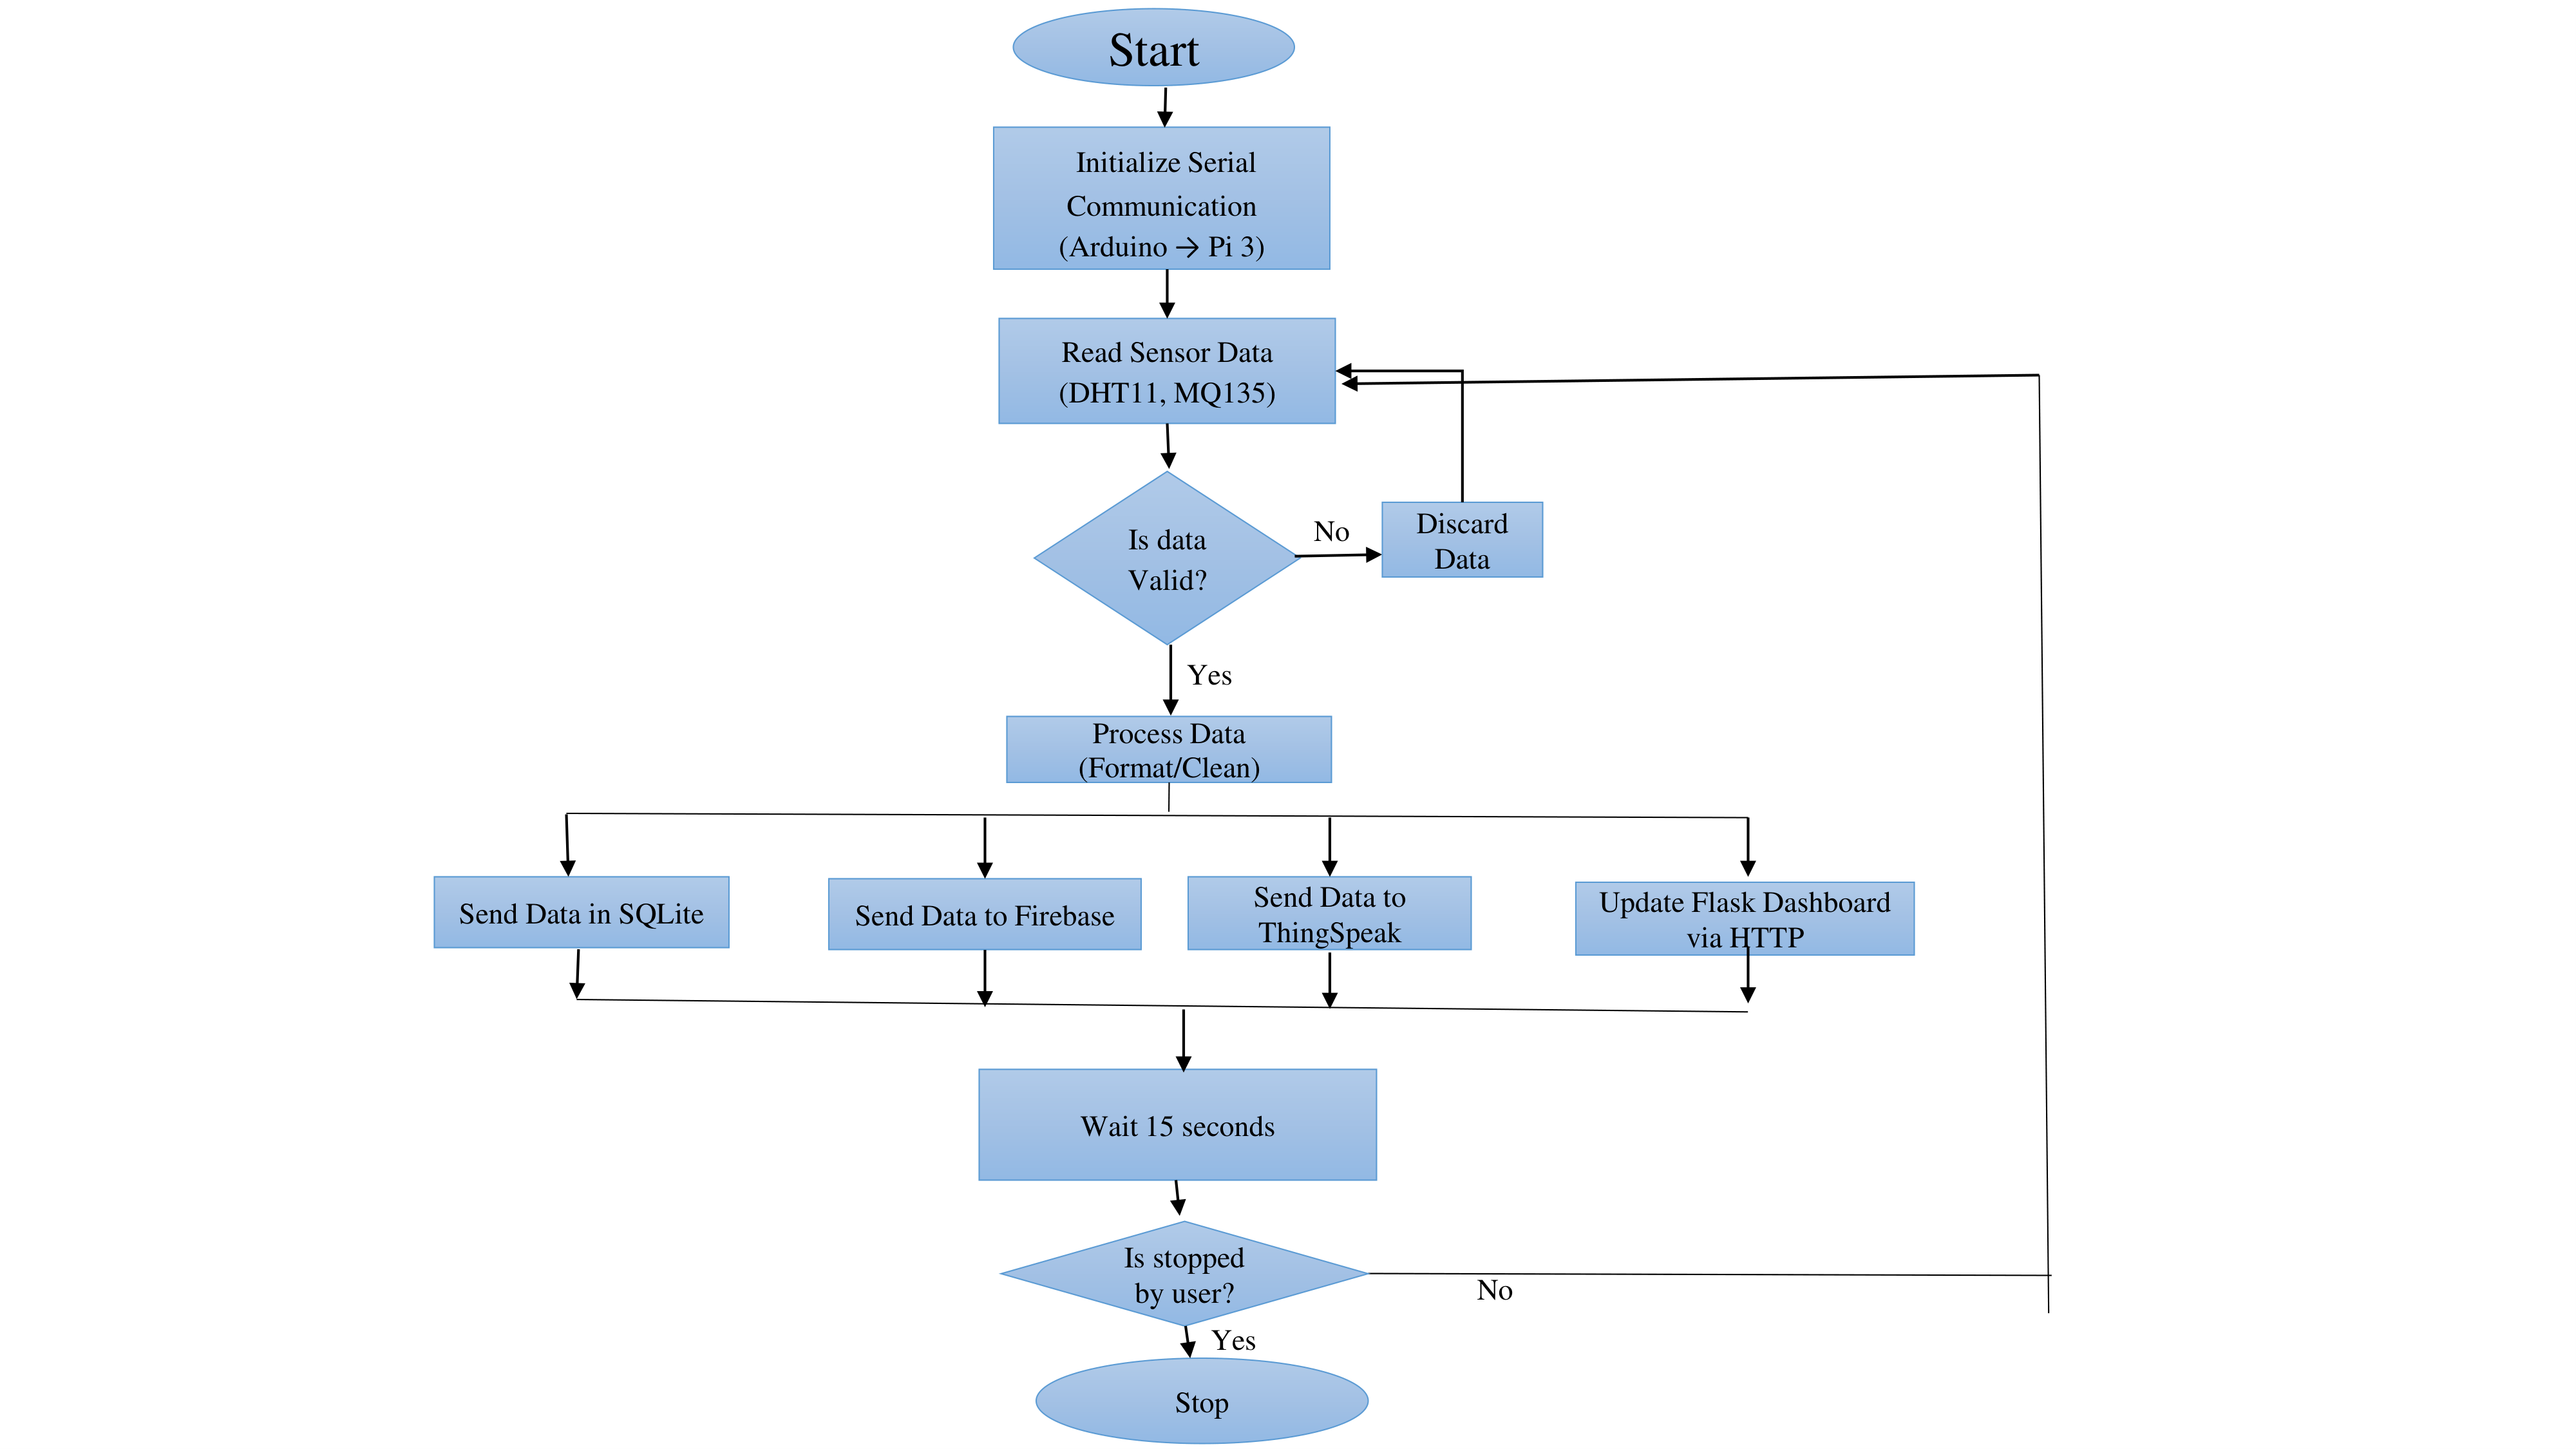
\includegraphics[
      width=1.3\textwidth,
      height=0.95\textheight,
      keepaspectratio
    ]{env_flowchart.png}%
  }
  \caption{Data flow of the environmental monitoring subsystem from sensor acquisition to cloud storage.}
  \label{fig:envflow}
\end{figure}

\subsection{Sensor Hardware and Integration}

The DHT11 temperature and humidity sensor measures ambient
temperature with accuracy $\pm 2\,^\circ$C and relative humidity with
accuracy $\pm 5\%$\,RH using a single-wire serial data protocol.

The MQ135 air quality gas sensor detects CO$_2$, ammonia,
benzene, and alcohol vapours through an electrochemical sensing element,
producing an analogue output voltage read by the Arduino UNO ADC as a
raw integer in the range 0 to 1023.

The Arduino UNO microcontroller reads both sensors at regular
intervals and transmits formatted serial strings at 9600 baud.

\subsection{Arduino Sensor Firmware}

The Arduino UNO firmware manages all sensor-level acquisition in the
environmental monitoring subsystem. The firmware is built around a simple
polling loop executing at a 5-second interval, matching the Raspberry Pi~3
processing rate and the ThingSpeak free-tier rate-limiting constraint.

The DHT11 sensor is interfaced through the \texttt{DHT} Arduino library.
Raw temperature ($T$) and humidity ($H$) values are validated against the
sensor's safe operating bounds before transmission:
$0^\circ\text{C}\le T\le 50^\circ\text{C}$ and
$20\,\%\text{RH}\le H\le 90\,\%\text{RH}$. If either value is
out-of-range or the DHT11 returns a NaN reading, the firmware transmits
an error marker and retries on the next cycle without corrupting the
Raspberry Pi~3 parser state.

The MQ135 sensor is sampled through \texttt{analogRead(A0)}, which
returns a 10-bit ADC integer in the range $[0,\,1023]$. No calibration
is performed on the Arduino; all calibration and classification logic
resides on the Raspberry Pi~3. This separation keeps the firmware simple
and the calibration parameters easy to update over SSH without
reflashing the microcontroller.

The formatted output follows the pattern
\texttt{T:\,<value>,H:\,<value>,AQ:\,<value>\textbackslash n}
transmitted at 9600\,baud. The Raspberry Pi~3 reads one line per
acquisition cycle, strips whitespace, splits on commas, and extracts the
three field values for the calibration pipeline.

Algorithm~\ref{alg:arduino} formalises the Arduino firmware state machine including warm-up, validation, and serial transmission. On power-on, the firmware initialises the DHT11 sensor on digital pin 2, configures the MQ135 analogue input on pin A0, and opens the serial port at 9600\,baud. A mandatory 2-second warm-up delay is imposed to allow the DHT11 to stabilise before the first reading is taken. The main acquisition loop then executes at a fixed 5-second interval. At each iteration, the firmware reads the temperature $T$ and humidity $H$ values from the DHT11 library and reads the 10-bit ADC value from the MQ135 sensor. Before transmitting any data, two validation checks are applied: if either $T$ or $H$ is not a number (\texttt{NaN}), an \texttt{ERROR:DHT\_FAULT} message is transmitted and the cycle is skipped; if either value falls outside the sensor's operating bounds ($0\le T\le 50\,^\circ$C and $20\le H\le 90$\,\%RH), an \texttt{ERROR:OUT\_OF\_RANGE} message is transmitted and the cycle is skipped. Only when both checks pass is the formatted string \texttt{T:\!<value>,H:\!<value>,AQ:\!<value>} transmitted over the serial connection to the Raspberry Pi~3 for calibration and classification.

\begin{algorithm}[H]
\DontPrintSemicolon
\caption{Arduino UNO Sensor Acquisition Firmware}
\label{alg:arduino}
\KwIn{DHT11 and MQ135 sensor signals}
\KwOut{Formatted serial string to Raspberry Pi~3 at 9600\,baud}
\BlankLine
\tcp{Setup (executes once on power-on)}
Initialise DHT11 on digital pin 2\;
Set MQ135 analogue input to pin A0\;
Configure serial port at 9600\,baud\;
$\texttt{delay}(2000\,\text{ms})$ \tcp*{sensor warm-up period}
\BlankLine
\tcp{Acquisition loop}
\While{powered}{
  $T\leftarrow\texttt{dht.readTemperature()}$\;
  $H\leftarrow\texttt{dht.readHumidity()}$\;
  $\text{AQ}\leftarrow\texttt{analogRead(A0)}$\;
  \BlankLine
  \If{$\texttt{isnan}(T)$ \textbf{or} $\texttt{isnan}(H)$}{
    $\texttt{Serial.println("ERROR:DHT\_FAULT")}$\; \textbf{continue}\;
  }
  \If{$T<0$ \textbf{or} $T>50$ \textbf{or} $H<20$ \textbf{or} $H>90$}{
    $\texttt{Serial.println("ERROR:OUT\_OF\_RANGE")}$\; \textbf{continue}\;
  }
  \BlankLine
  $\text{msg}\leftarrow\texttt{"T:"}+T+\texttt{",H:"}+H+\texttt{",AQ:"}+\text{AQ}$\;
  $\texttt{Serial.println}(\text{msg})$ \tcp*{transmit to Raspberry Pi~3}
  $\texttt{delay}(5000\,\text{ms})$ \tcp*{5-second acquisition interval}
}
\end{algorithm}

The \textbf{Raspberry Pi~3} receives and parses the serial stream,
performs calibration, executes the alert logic, and manages all four
output channels.

\subsection{AQ-to-CO$_2$ Calibration}

The MQ135 sensor outputs a raw ADC value proportional to aggregate
gas concentration rather than a direct CO$_2$ reading. A linear
interpolation formula, based on the MQ135 sensor characterisation
described in \cite{r50,r1,r2}, maps this raw value to an estimated
CO$_2$ concentration in parts per million (Equation~\eqref{eq:co2}):

\begin{equation}
  \text{CO}_2\,(\text{ppm}) = \text{CO}_{2,\min}
  + \frac{(\text{AQ}_\text{raw} - \text{AQ}_\text{clean})}
         {(\text{AQ}_\text{max} - \text{AQ}_\text{clean})}
  \times (\text{CO}_{2,\max} - \text{CO}_{2,\min})
  \label{eq:co2}
\end{equation}

The calibration constants are: $\text{AQ}_\text{clean} = 38$ (sensor
reading in fresh outdoor air after a 24-hour warm-up period),
$\text{AQ}_\text{max} = 650$, $\text{CO}_{2,\min} = 350\,\text{ppm}$
(typical ambient outdoor concentration), and
$\text{CO}_{2,\max} = 2500\,\text{ppm}$. The computed value is clamped
to the range $[350,\,2500]$\,ppm \cite{r50,r1,r2}.

\subsection{Data Processing and Alert Logic}

After calibration, each reading is passed through a sensor fault
validation check and then classified using a six-level priority-ordered
alert hierarchy. The classification thresholds are grounded in
established indoor air quality standards. ASHRAE Standard~62.1
\cite{r46} specifies that CO$_2$ in occupied indoor spaces should not
exceed approximately 1100\,ppm (700\,ppm above the outdoor ambient
concentration of $\sim$400\,ppm). The WHO Indoor Air Quality Guidelines
\cite{r47} and supporting epidemiological research \cite{r48,r49}
indicate that CO$_2$ concentrations above 1000\,ppm are associated with
noticeably reduced air quality and early health effects, while levels
above 2000\,ppm are considered poor and require immediate action.

Table~\ref{tab:alertlevels} summarises the CO$_2$ thresholds and
corresponding alert levels implemented in the system.

\begin{table}[tbp]
  \centering
  \caption{CO$_2$ concentration thresholds and alert classifications.}
  \label{tab:alertlevels}
  \begin{tabular}{lll}
    \toprule
    Alert Level    & CO$_2$ Range (ppm)  & Action \\
    \midrule
    OK             & $< 600$             & Conditions nominal; no action needed \\
    VENTILATION    & $600$--$1000$       & Air quality declining; increase ventilation \\
    WARNING        & $1000$--$1500$      & Elevated CO$_2$; monitor closely \\
    CRITICAL       & $1500$--$2000$      & Hazardous classification; ventilate immediately \\
    CRITICAL+      & $> 2000$            & Severe; possible gas leak or equipment fault \\
    HARDWARE       & Any                 & Sensor fault; temperature or humidity out of range \\
    \bottomrule
  \end{tabular}
\end{table}

The six-level classification hierarchy, in descending priority order, is:

\begin{enumerate}
  \item \textbf{HARDWARE:} The DHT11 returned a value outside its
        valid range, indicating a sensor fault or wiring issue.
  \item \textbf{CRITICAL+:} CO$_2$ exceeds 2000\,ppm; severe
        conditions requiring immediate action \cite{r47,r48}.
  \item \textbf{CRITICAL:} CO$_2$ in the 1500--2000\,ppm range;
        ventilate the space immediately \cite{r47}.
  \item \textbf{WARNING:} CO$_2$ in the 1000--1500\,ppm range;
        air quality is declining and should be monitored \cite{r48,r49}.
  \item \textbf{VENTILATION:} CO$_2$ in the 600--1000\,ppm range;
        increase ventilation to prevent further rise \cite{r46}.
  \item \textbf{OK:} All sensor values within nominal ranges and
        CO$_2$ below 600\,ppm.
\end{enumerate}

Algorithm~\ref{alg:envpipeline} formalises the complete data acquisition and dispatch pipeline executed on the Raspberry Pi~3. The pipeline begins by initialising the SQLite database schema and opening the serial connection to the Arduino UNO at \texttt{/dev/ttyACM0} at 9600\,baud. A background Flask server is launched on \texttt{0.0.0.0:5000} to serve the live dashboard. Within the main acquisition loop, each line received from the serial port is checked for the expected \texttt{T:} prefix; malformed or error lines are discarded without disrupting the loop. Valid lines are parsed to extract $T$, $H$, and the raw AQ value. If the sensor values are out of range, the alert level is immediately set to \texttt{HARDWARE}. Otherwise, the raw AQ value is converted to an estimated CO$_2$ concentration using Equation~\eqref{eq:co2}, and the resulting value is passed to the six-level classification logic. After classification, the processed reading is dispatched simultaneously to four output channels: SQLite local storage, the Firebase Realtime Database cloud node, the ThingSpeak IoT platform (subject to the 15-second rate-limiting guard), and the Flask dashboard state. The loop then waits 15\,s before the next acquisition cycle.

Algorithm~\ref{alg:alert} details the six-level priority-ordered alert classification applied to every processed CO$_2$ reading. The classification is performed in strict priority order from the most severe condition to the most benign. The highest priority level, \texttt{HARDWARE}, is triggered when the sensor fault flag $f = 1$, indicating that the DHT11 reported an out-of-range or \texttt{NaN} reading in the current cycle. If no hardware fault is present, the CO$_2$ concentration is compared against four descending thresholds: \texttt{CRITICAL+} for values above 2000\,ppm \cite{r47,r48}, \texttt{CRITICAL} for values between 1500 and 2000\,ppm \cite{r47}, \texttt{WARNING} for values between 1000 and 1500\,ppm \cite{r48,r49}, and \texttt{VENTILATION} for values between 600 and 1000\,ppm \cite{r46}. If none of these thresholds are exceeded, the reading is classified as \texttt{OK}, indicating that all sensor values are within their nominal operating ranges.

\begin{algorithm}[H]
\DontPrintSemicolon
\caption{Environmental Monitoring Acquisition and Dispatch Pipeline}
\label{alg:envpipeline}
\KwIn{Serial stream from Arduino UNO}
\KwOut{Readings persisted to SQLite, Firebase, ThingSpeak, and Flask}
\BlankLine
Initialise SQLite schema via \texttt{init\_db()}\;
Open serial port \texttt{/dev/ttyACM0} at 9600\,baud (PySerial)\;
Start Flask server on \texttt{0.0.0.0:5000} in background thread\;
\BlankLine
\While{not stopped}{
  $\text{line}\leftarrow\texttt{serial.readline().decode().strip()}$\;
  \If{not $\text{line.startswith("T:")}$}{
    \textbf{continue} \tcp*{discard malformed or error lines}
  }
  Parse: $T,\,H,\,\text{AQ}\leftarrow\texttt{parse}(\text{line})$\;
  \BlankLine
  \If{$T<0$ \textbf{or} $T>50$ \textbf{or} $H<20$ \textbf{or} $H>90$}{
    $\text{alert}\leftarrow\texttt{HARDWARE}$\;
  }\Else{
    $\text{CO}_2\leftarrow\texttt{calibrate}(\text{AQ})$ \tcp*{Equation~\ref{eq:co2}}
    $\text{alert}\leftarrow\texttt{ClassifyAlert}(\text{CO}_2)$ \tcp*{Algorithm~\ref{alg:alert}}
  }
  \BlankLine
  \tcp{Parallel four-channel dispatch}
  \texttt{SQLiteWrite}$(T,\,H,\,\text{AQ},\,\text{CO}_2,\,\text{alert})$\;
  \texttt{FirebasePush}$(T,\,H,\,\text{AQ},\,\text{CO}_2,\,\text{alert})$ \tcp*{daemon thread; non-blocking}
  \If{$\Delta t_{\text{ThingSpeak}}\geq 15\,\text{s}$}{
    \texttt{ThingSpeakSend}$(T,\,H,\,\text{CO}_2,\,\text{AQ})$\;
  }
  \texttt{FlaskUpdate}$\text{(latest\_reading)}$\;
  $\texttt{sleep}(15\,\text{s})$ \tcp*{rate-limiter guard}
}
\end{algorithm}

\begin{algorithm}[H]
\DontPrintSemicolon
\caption{Six-Level CO$_2$ Alert Classification (Priority-Ordered)}
\label{alg:alert}
\KwIn{$\text{CO}_2$ concentration (ppm), sensor fault flag $f\in\{0,1\}$}
\KwOut{Alert level string}
\BlankLine
\If{$f=1$}{
  \Return \texttt{HARDWARE} \tcp*{sensor fault or out-of-range reading}
}
\If{$\text{CO}_2>2000$}{
  \Return \texttt{CRITICAL+} \tcp*{severe \cite{r47,r48}}
}
\If{$1500<\text{CO}_2\leq 2000$}{
  \Return \texttt{CRITICAL} \tcp*{ventilate immediately \cite{r47}}
}
\If{$1000<\text{CO}_2\leq 1500$}{
  \Return \texttt{WARNING} \tcp*{monitor closely \cite{r48,r49}}
}
\If{$600<\text{CO}_2\leq 1000$}{
  \Return \texttt{VENTILATION} \tcp*{increase ventilation \cite{r46}}
}
\Return \texttt{OK} \tcp*{all readings nominal}
\end{algorithm}



\subsection{Multi-Channel Data Storage and Cloud Transmission}

Each processed reading is written to four parallel output channels
concurrently, as shown in Figure~\ref{fig:envflow}.

\textbf{SQLite Local Storage} writes each reading to a
\texttt{readings} table containing 14 fields. All Flask dashboard
queries are served from SQLite to ensure responsiveness independent
of cloud connectivity \cite{r23}.

\textbf{Firebase Realtime Database} \cite{r35} receives each reading
via the \texttt{firebase\_admin} Python SDK \cite{r45}, pushed to the
\texttt{/readings} node in a daemon background thread to ensure that
network timeouts never block the acquisition loop \cite{r2}.

\textbf{ThingSpeak IoT Platform} \cite{r36} receives sensor readings
via HTTP GET with six field mappings for temperature, humidity,
CO$_2$~ppm, raw AQ, cluster label, and anomaly flag. A 15-second
rate-limiting guard enforces the ThingSpeak free-tier constraint
\cite{r1,r23}.

\textbf{Flask Live Dashboard} \cite{r37} serves a real-time HTML
monitoring interface at \texttt{http://<Pi-IP>:5000} with three REST
endpoints: \texttt{/api/latest}, \texttt{/api/history}, and
\texttt{/api/alerts}.

\subsection{System Startup and Orchestration}

The \texttt{main.py} entry point initialises the SQLite schema through
\texttt{init\_db()}, launches the serial reader as a background daemon
thread, and starts the Flask server on \texttt{0.0.0.0:5000}. The
serial reader implements an outer reconnection loop: if the USB
connection is lost, the thread waits five seconds and then attempts
automatic port re-detection and reconnection.

\section{Integrated System Summary}

The complete framework integrates the autonomous robot subsystem managed
by the Raspberry Pi~5 and the environmental monitoring subsystem managed
by the Raspberry Pi~3 on a single mobile chassis. Both subsystems
operate concurrently and independently on separate processors, so that
computational load or software events in one subsystem do not affect
the real-time performance of the other. This modular two-processor
architecture directly supports the scalability, maintainability, and
operational reliability goals of the proposed framework
\cite{r23,r26,r29}.
% ── Chapter 4: Results and Discussion ────────────────────────

\chapter{Results and Discussion}

This chapter presents the experimental results obtained from the two
principal subsystems of the proposed framework. Section~\ref{sec:nav}
presents the quantitative performance evaluation of vision-based
autonomous path following. Section~\ref{sec:env} presents the
real-time sensor data acquisition, cloud transmission, and dashboard
results. Section~\ref{sec:disc} provides a consolidated discussion,
and Section~\ref{sec:lim} identifies the limitations of the current
implementation.

\section{Vision-Based Autonomous Path Following}
\label{sec:nav}

\subsection{Experimental Setup and Performance Metrics}

All path-following experiments were conducted on a closed rectangular
trajectory of 152.4\,cm $\times$ 91.44\,cm constructed using red
adhesive tape on a tiled indoor floor, with a total perimeter of
487.68\,cm. Figure~\ref{fig:robotpath} shows the experimental path.
A total of 40 trials were performed: 20 under manual teleoperation
and 20 under autonomous vision-based navigation, under identical
lighting and environmental conditions.

\begin{figure}[tbp]
  \centering
  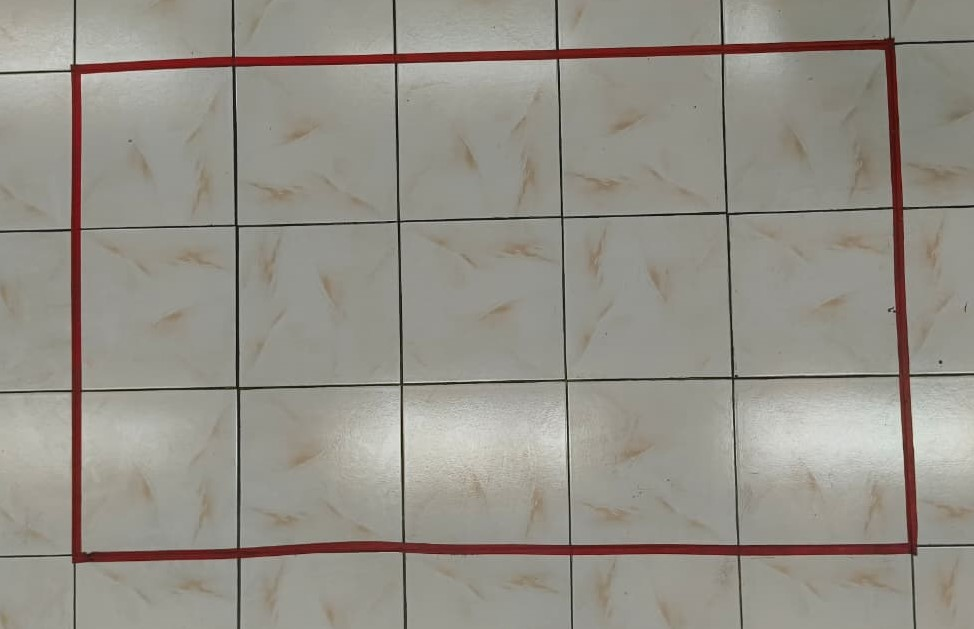
\includegraphics[width=0.82\textwidth]{WhatsApp Image 2026-04-10 at 1.09.01 PM (2).jpeg}
  \caption{Rectangular red tape path on tiled floor used for all 40 experimental trials.}
  \label{fig:robotpath}
\end{figure}

The primary performance metric is the Root Mean Square Error (RMSE)
of lateral deviation. The RMSE is a standard measure of tracking
accuracy in mobile robot navigation, and is computed per trial as
given in Equation~\eqref{eq:rmse}:

\begin{equation}
  \text{RMSE} = \sqrt{\frac{1}{N}\sum_{i=1}^{N} e_i^2}
  \label{eq:rmse}
\end{equation}

\noindent where $e_i$ is the instantaneous lateral tracking error at
sample $i$ and $N$ is the total number of recorded samples.
The sample mean error and standard deviation of tracking errors are
defined in Equation~\eqref{eq:mean_std} as:

\begin{equation}
  \bar{e} = \frac{1}{N}\sum_{i=1}^{N} e_i, \qquad
  \sigma  = \sqrt{\frac{1}{N}\sum_{i=1}^{N}(e_i - \bar{e})^2}
  \label{eq:mean_std}
\end{equation}

\noindent where $\bar{e}$ is the sample mean and $\sigma$ the standard
deviation of the instantaneous lateral tracking errors across a trial.

The maximum possible lateral deviation, corresponding to half the path
width, is given in Equation~\eqref{eq:emax}:

\begin{equation}
  E_{\max} = \frac{W}{2} = \frac{91.44}{2} = 45.72\,\text{cm}
  \label{eq:emax}
\end{equation}

\noindent where $W$ is the physical path width in centimetres.
Using Equation~\eqref{eq:emax}, the normalised tracking error and
tracking accuracy are computed in Equation~\eqref{eq:accuracy} as:

\begin{equation}
  E_{\text{norm}} = \frac{\text{RMSE}}{E_{\max}}, \qquad
  \text{Accuracy} = 1 - E_{\text{norm}}
  \label{eq:accuracy}
\end{equation}

\noindent where tracking accuracy is expressed as the proportion of
the path width that the robot maintains.

\subsection{Trajectory Analysis and Descriptive Statistics}

Figure~\ref{fig:traj_best} presents the best-performing trial pair:
manual trial~18 (RMSE = 14.75\,cm) against autonomous run~19
(RMSE = 1.489\,cm). The manual trajectory shows noticeable outward
deviation at all four straight segments and corner transitions.
Autonomous run~19 stays remarkably close to the reference line
throughout the entire lap.

\begin{figure}[tbp]
  \centering
  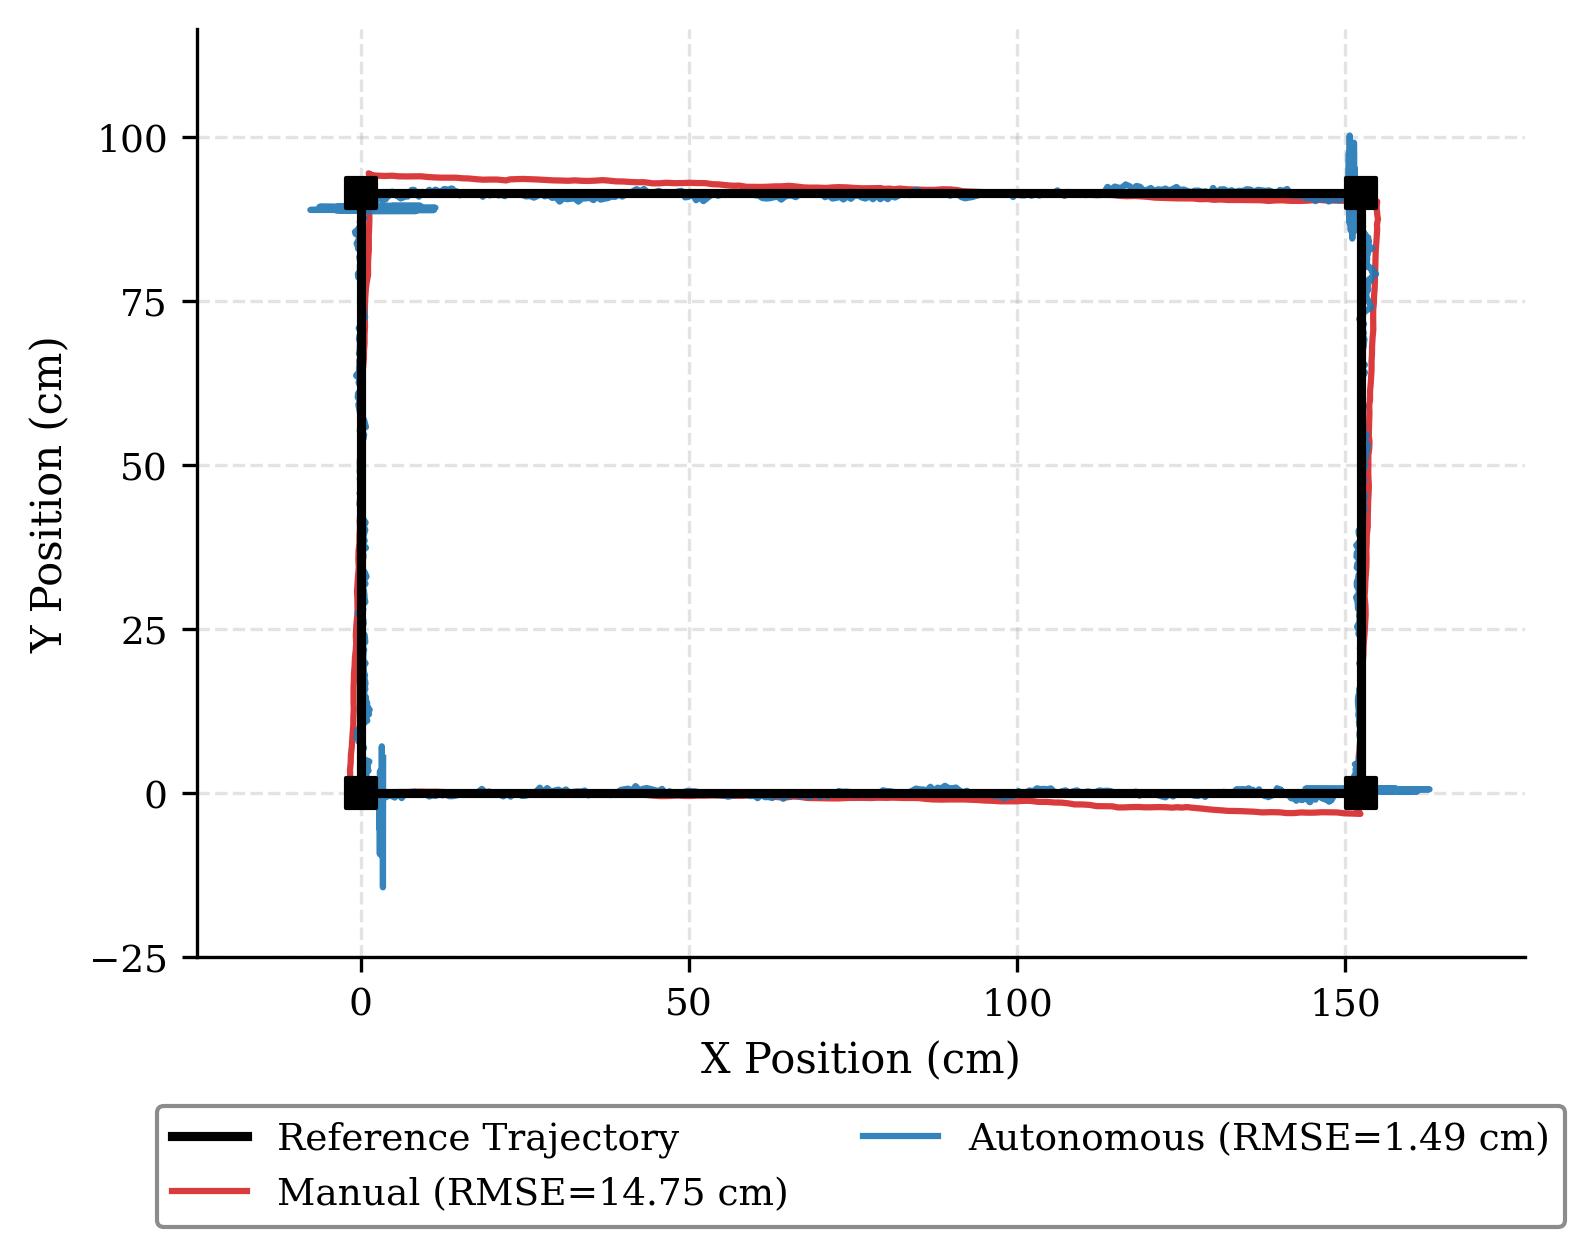
\includegraphics[width=0.90\textwidth]{plot_path_best.png}
  \caption{Best-case trajectory pair: manual trial~18 vs.\ autonomous run~19 overlaid on the reference path.}
  \label{fig:traj_best}
\end{figure}

Figure~\ref{fig:traj_worst} presents all 20 autonomous trajectories
overlaid on the reference path. Even the worst autonomous trial
(run~20, RMSE = 5.554\,cm) is considerably lower than the best manual
trial ever recorded (14.751\,cm), a difference of over 9\,cm, which
confirms that the two distributions do not overlap at all.

\begin{figure}[tbp]
  \centering
  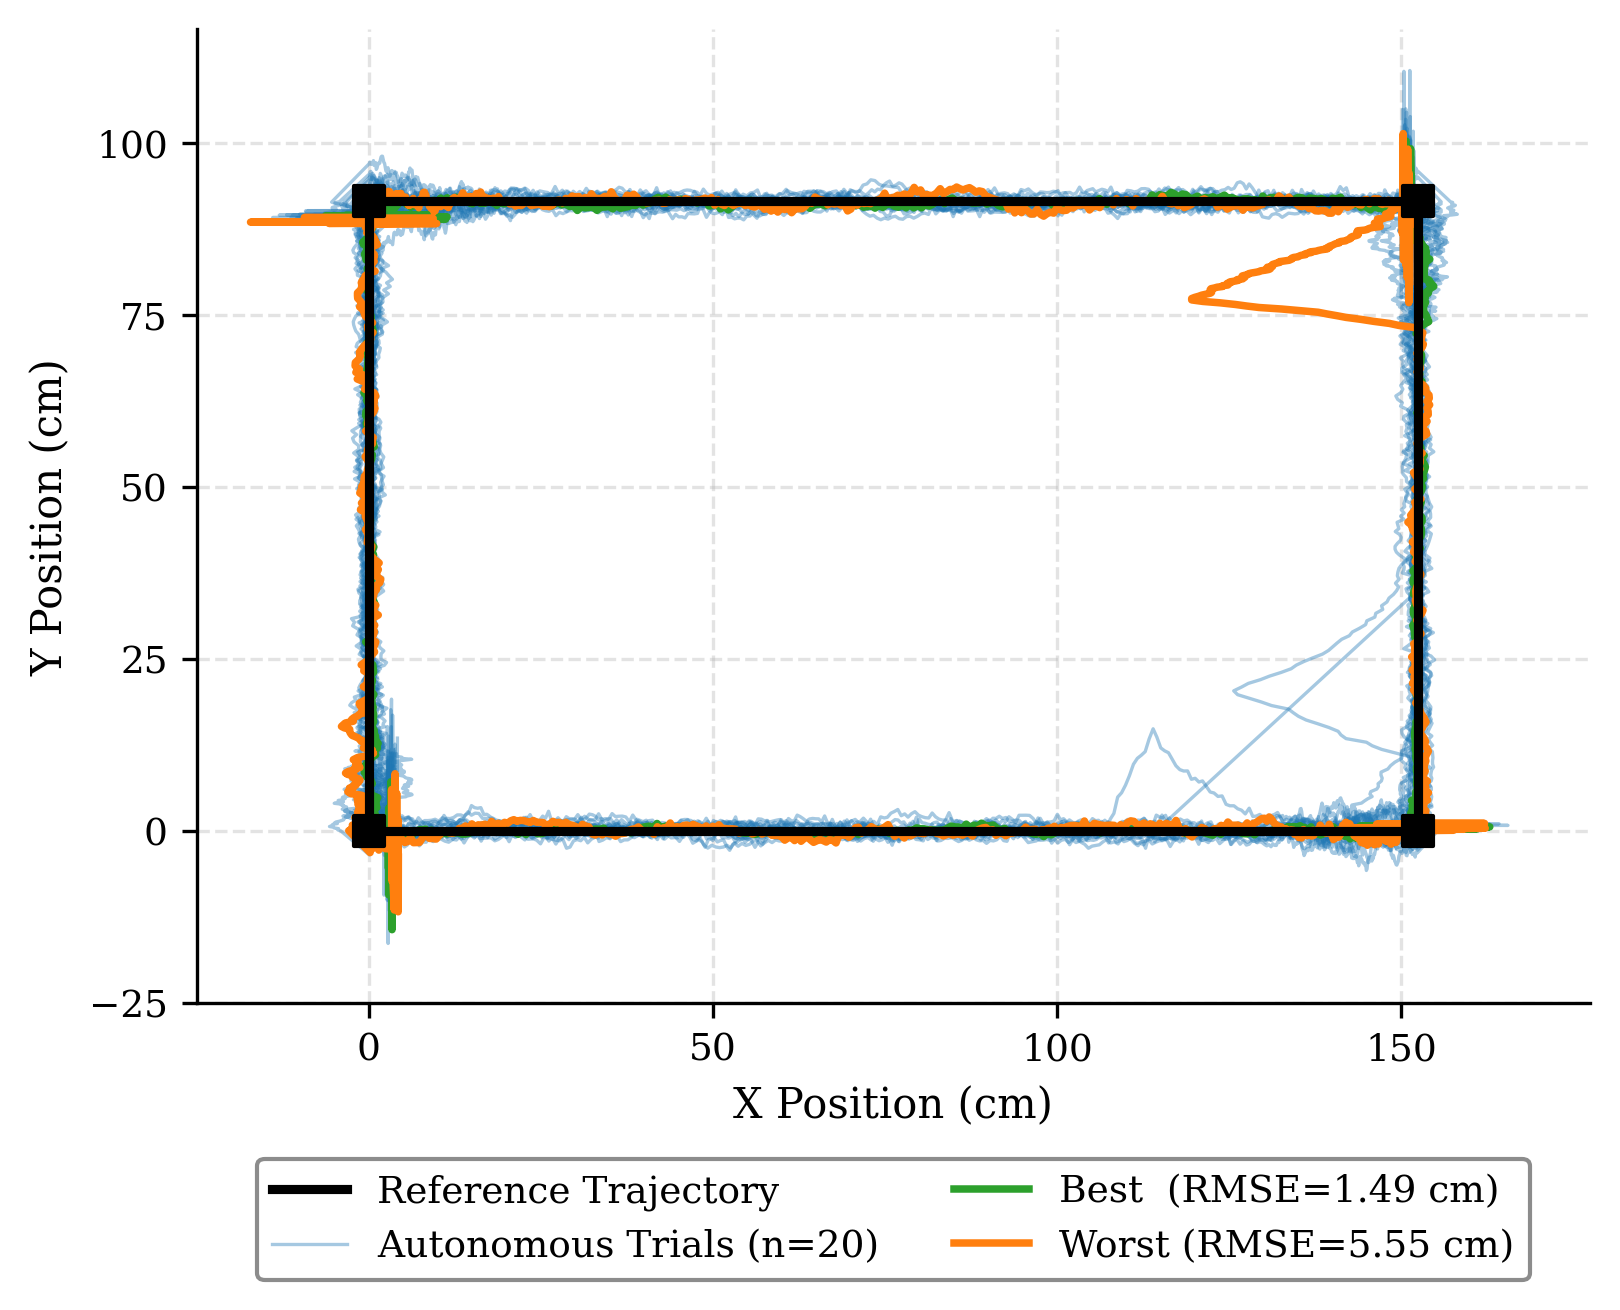
\includegraphics[width=0.90\textwidth]{plot_path_all_autonomous.png}
  \caption{All 20 autonomous trial trajectories overlaid on the reference path. The worst autonomous trial (run~20, 5.55\,cm) remains below the best manual trial (14.75\,cm).}
  \label{fig:traj_worst}
\end{figure}

Table~\ref{tab:desc_stats} presents the per-trial RMSE summary
statistics. The autonomous mode achieves a mean RMSE of 2.222\,cm,
an 86.75\% reduction from the manual mean of 16.768\,cm.
Even the worst 5\% of autonomous trials (95th percentile = 4.087\,cm)
fell well below the best manual trial ever recorded (14.751\,cm),
demonstrating consistent superiority of closed-loop autonomous
control over manual teleoperation.

\begin{table}[tbp]
  \centering
  \caption{Per-trial RMSE descriptive statistics for both operating modes ($n=20$, values in cm).}
  \label{tab:desc_stats}
  \begin{tabular}{lcccc}
    \toprule
    Metric          & Manual & Autonomous & Reduction & Reduction (\%) \\
    \midrule
    Mean RMSE       & 16.768 & 2.222      & 14.546    & 86.75\% \\
    Median RMSE     & 16.211 & 1.980      & 14.231    & 87.8\%  \\
    Std Deviation   & 2.101  & 0.958      & 1.143     & 54.4\%  \\
    Minimum         & 14.751 & 1.489      & 13.262    & --      \\
    Maximum         & 23.147 & 5.554      & 17.593    & 76.0\%  \\
    95th Percentile & 19.969 & 4.087      & 15.882    & 79.5\%  \\
    \bottomrule
    \multicolumn{5}{l}{\small $n = 20$ trials each $|$ 5\,ft $\times$ 3\,ft Rectangular Path}
  \end{tabular}
\end{table}

\subsection{Temporal Error Behaviour and Error Distribution}

Figure~\ref{fig:rmse_bar} presents the per-trial RMSE values for all
40 trials. Manual RMSE values range from 14.751\,cm to 23.147\,cm.
Autonomous RMSE values are consistently low, ranging from 1.365\,cm
to 5.588\,cm across all 20 trials, with no overlap between the two
distributions.

\begin{figure}[tbp]
  \centering
  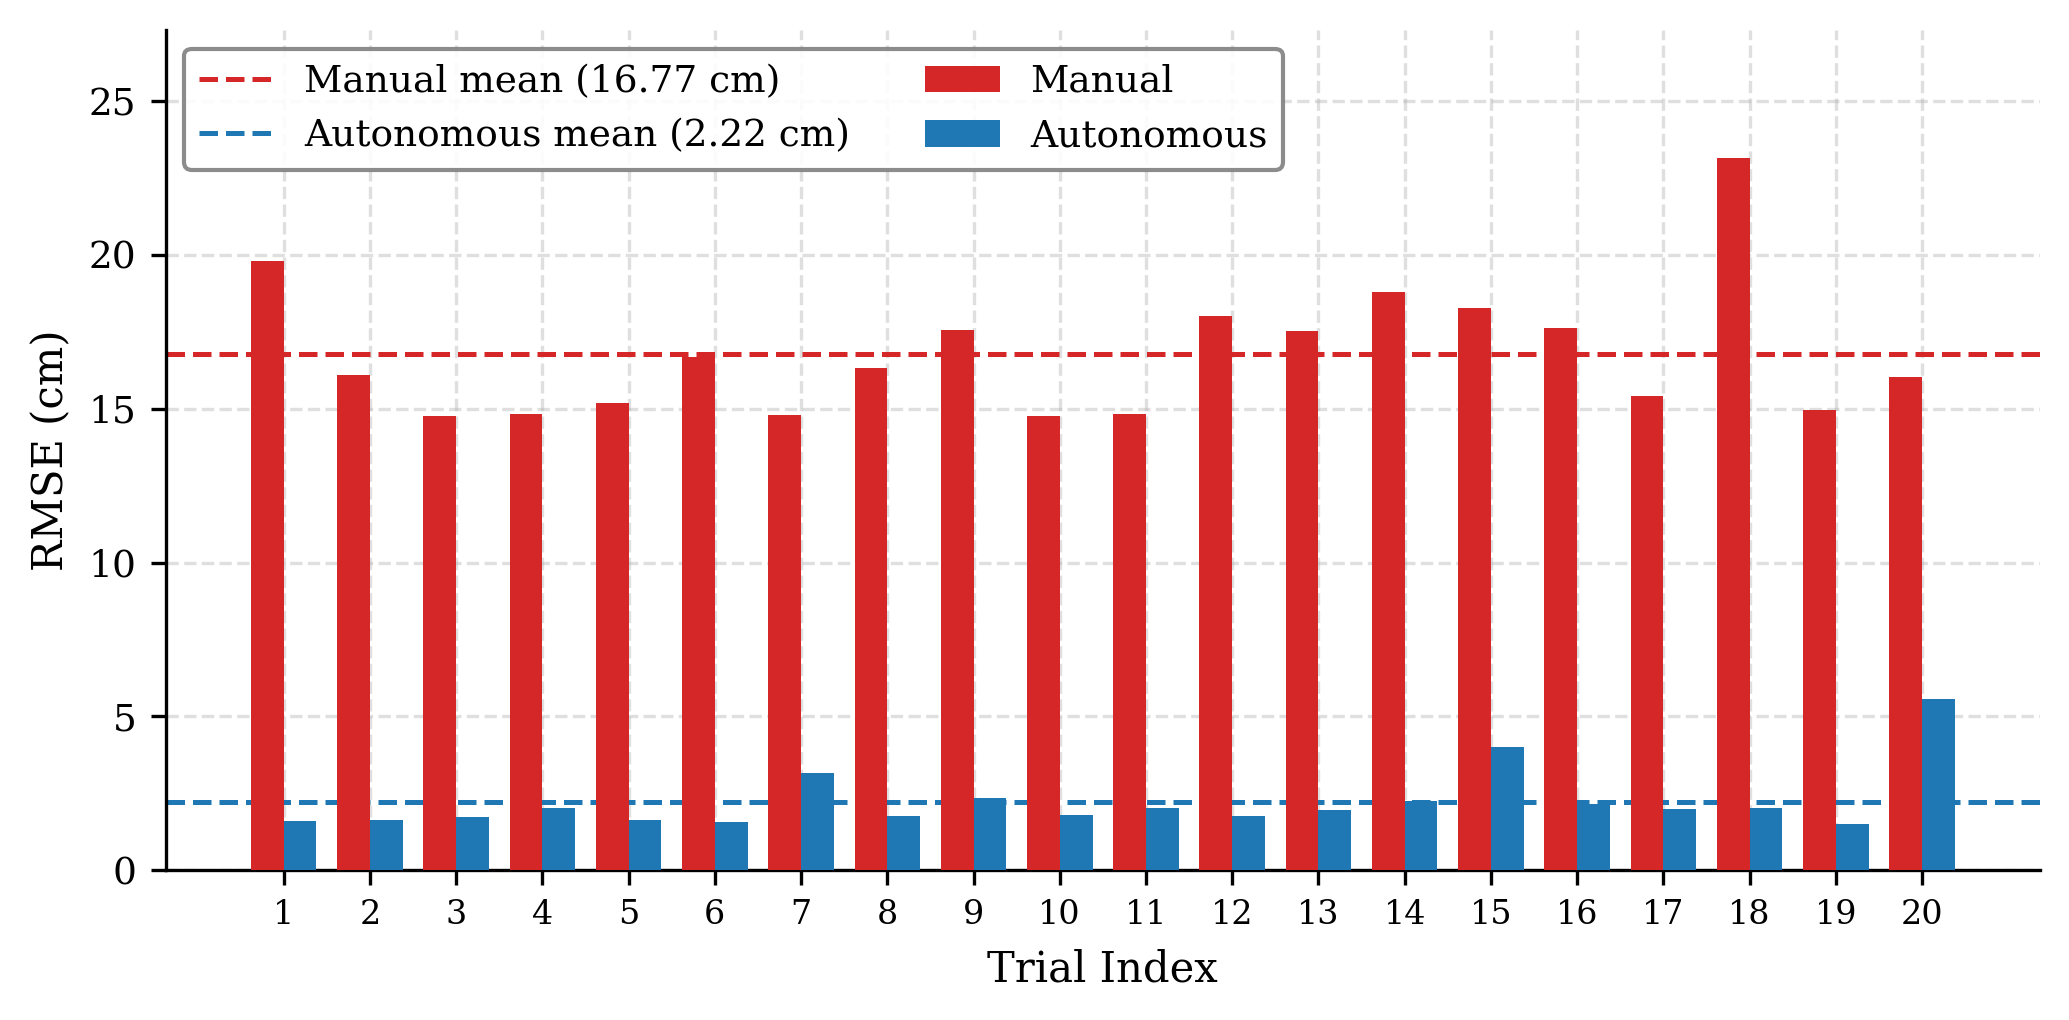
\includegraphics[width=0.88\textwidth]{plot_per_trial_rmse_bar.png}
  \caption{Per-trial RMSE for all 20 manual and 20 autonomous trials. No autonomous trial exceeds 5.55\,cm; no manual trial falls below 14.75\,cm.}
  \label{fig:rmse_bar}
\end{figure}

Figure~\ref{fig:error_time} shows the temporal evolution of tracking
error for the best trial in each mode. The manual trace fluctuates
within approximately 10 to 16\,cm. The autonomous trace maintains
near-zero error throughout all four straight segments with narrow
spikes only at corner transitions, confirming the effectiveness of
the PID derivative term in damping rapid deviation changes.

\begin{figure}[tbp]
  \centering
  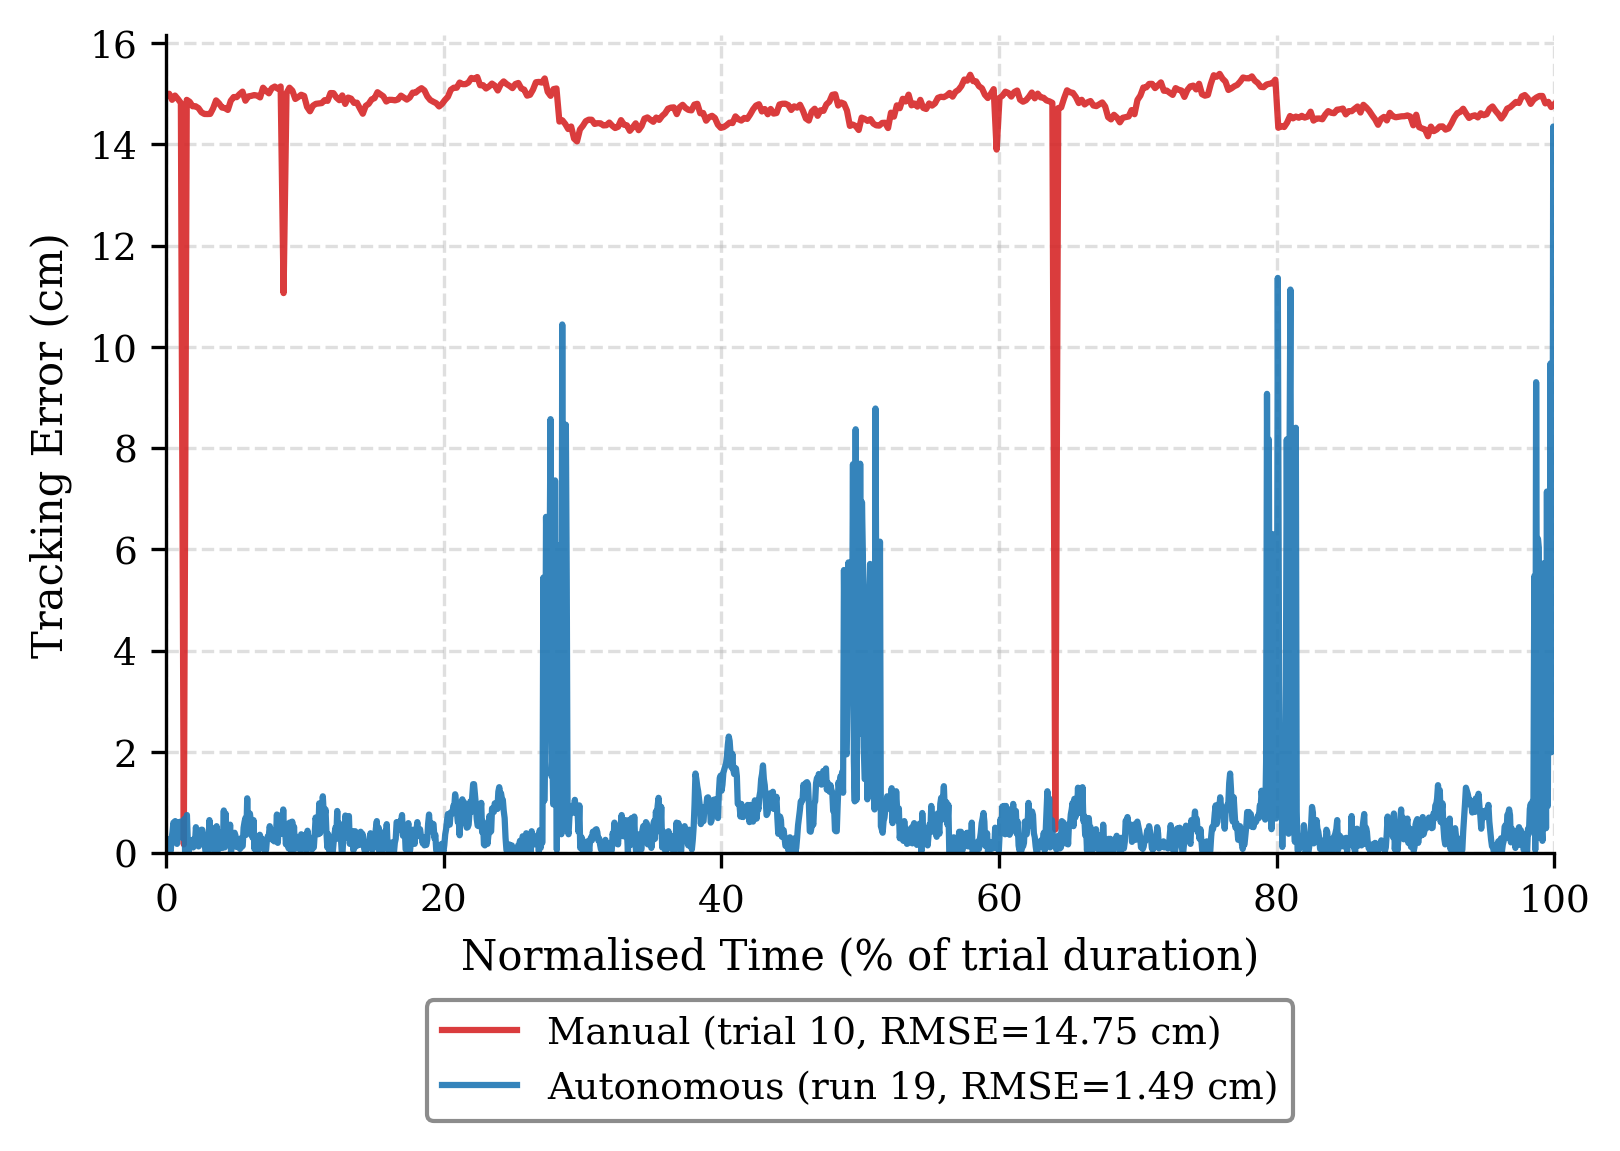
\includegraphics[width=0.88\textwidth]{plot_error_over_time_best.png}
  \caption{Tracking error over normalised trial time for the best manual (trial~18) and best autonomous (run~19) trial.}
  \label{fig:error_time}
\end{figure}

Figure~\ref{fig:histogram} presents the probability distribution of
instantaneous tracking errors. The manual distribution is broad,
centred near 15\,cm. The autonomous distribution is narrow and sharply
peaked near 0\,cm, confirming systematic improvement.

\begin{figure}[tbp]
  \centering
  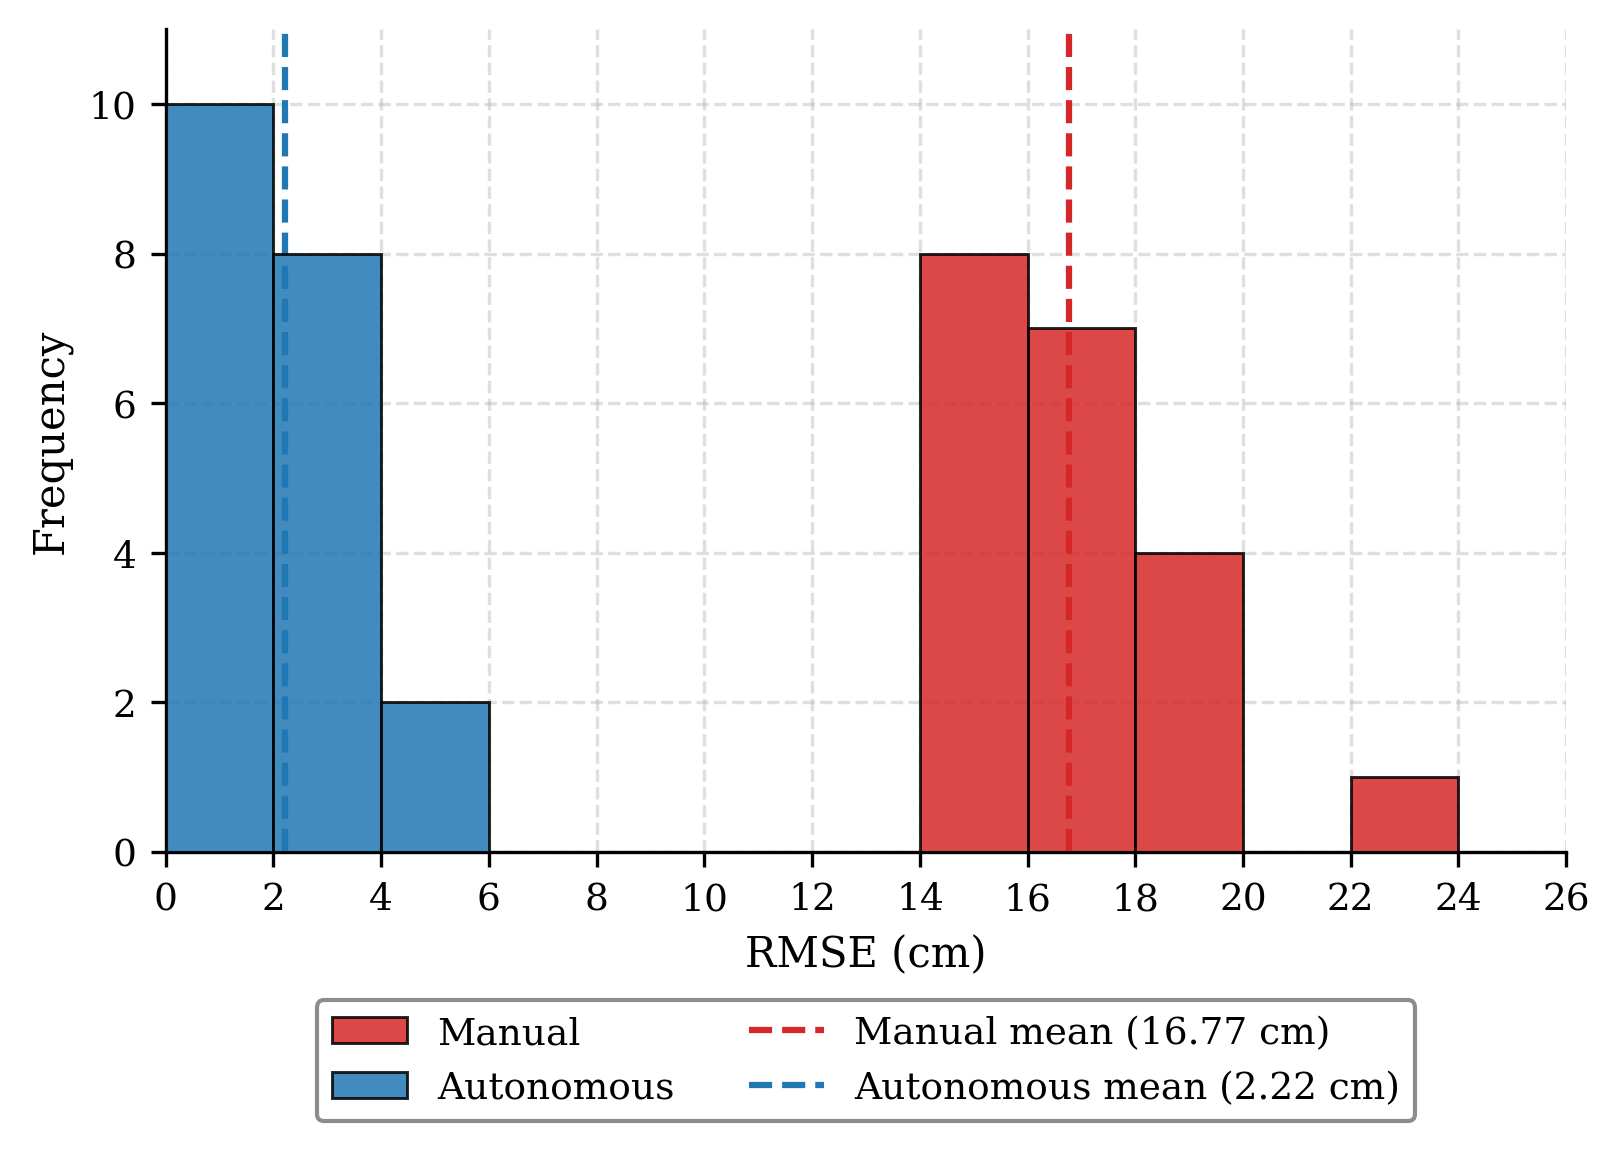
\includegraphics[width=0.85\textwidth]{plot_histogram.png}
  \caption{Probability distribution of instantaneous tracking errors for manual and autonomous modes.}
  \label{fig:histogram}
\end{figure}

Figure~\ref{fig:cdf} presents the cumulative distribution function
of per-trial RMSE for both modes. The autonomous distribution rises
steeply and reaches its maximum at 5.588\,cm, well before the manual
distribution begins to rise from 14.751\,cm, demonstrating complete
stochastic dominance of autonomous over manual performance.

\begin{figure}[tbp]
  \centering
  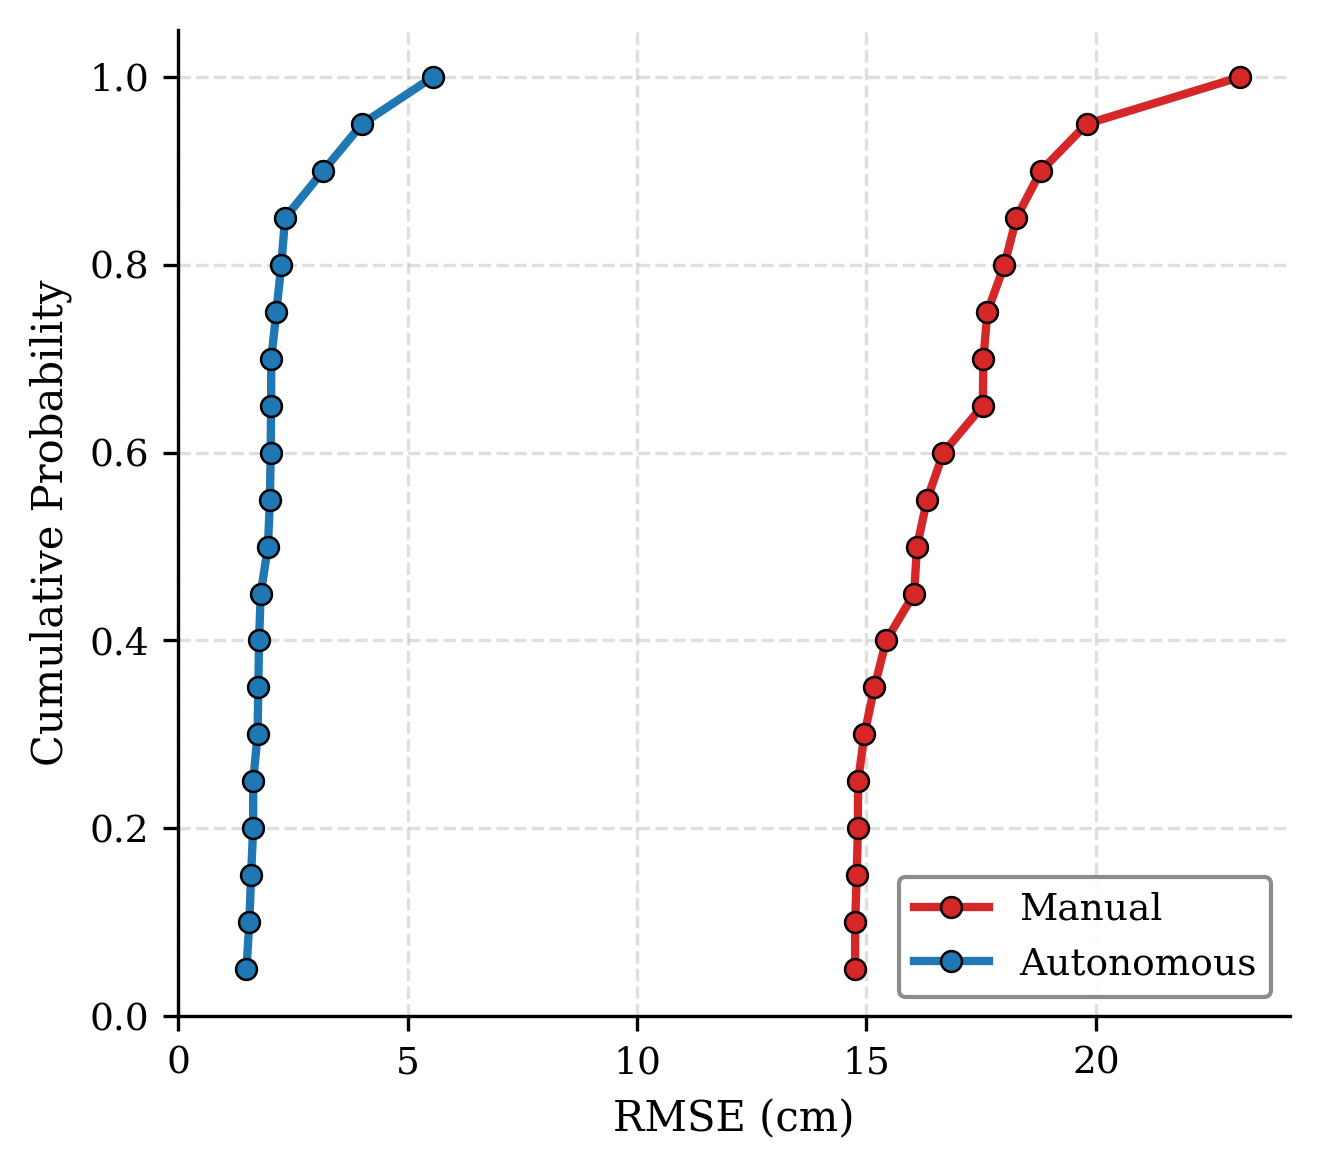
\includegraphics[width=0.82\textwidth]{plot_cdf.png}
  \caption{Cumulative distribution function of per-trial RMSE for manual and autonomous modes, showing complete stochastic dominance of autonomous over manual.}
  \label{fig:cdf}
\end{figure}

\subsection{Accuracy Analysis}

Using Equation~\eqref{eq:accuracy}, Table~\ref{tab:accuracy} presents
the tracking accuracy results. The autonomous mode achieves a mean
tracking accuracy of 95.14\%, compared with 63.33\% for manual
teleoperation, a gain of 31.81 percentage points.

\begin{table}[tbp]
  \centering
  \caption{Tracking accuracy analysis ($E_{\max} = 45.72$\,cm, $n=20$ each).}
  \label{tab:accuracy}
  \begin{tabular}{lcccc}
    \toprule
    Mode       & Mean RMSE (cm) & Norm.\ Error & Accuracy (\%) & Gain \\
    \midrule
    Manual     & 16.768         & 0.3668       & 63.33\%       & --       \\
    Autonomous & 2.222          & 0.0486       & 95.14\%       & +31.81\% \\
    \bottomrule
  \end{tabular}
\end{table}

\subsection{Statistical Validation}

The statistical analysis proceeds in four stages. The results are
presented below in order of normality testing, hypothesis testing,
effect size measurement, and bootstrap confidence interval estimation.

\paragraph{Normality Testing.}
The Shapiro--Wilk test was applied to both distributions
to determine whether parametric or non-parametric tests are appropriate.
Table~\ref{tab:normality} confirms that both distributions are
non-normal ($p < 0.05$), justifying the use of non-parametric tests.

\begin{table}[tbp]
  \centering
  \caption{Shapiro--Wilk normality test results for per-trial RMSE.}
  \label{tab:normality}
  \begin{tabular}{lcccc}
    \toprule
    Mode       & $W$    & $p$-value & Normal?         & Action \\
    \midrule
    Manual     & 0.8502 & 0.0054    & No ($p < 0.05$) & Non-parametric test \\
    Autonomous & 0.6564 & 0.000012  & No ($p < 0.05$) & Non-parametric test \\
    \bottomrule
  \end{tabular}
\end{table}

\paragraph{Significance Testing.}
Table~\ref{tab:significance} presents four independent hypothesis
tests for $H_0$: Manual RMSE $\leq$ Autonomous RMSE versus $H_1$:
Manual RMSE $>$ Autonomous RMSE. All four tests unanimously reject
$H_0$ with $p$-values many orders of magnitude below the conventional
threshold of $\alpha = 0.05$.

\begin{table}[tbp]
  \centering
  \caption{Significance testing results ($H_1$: Manual RMSE $>$ Autonomous RMSE).}
  \label{tab:significance}
  \resizebox{\textwidth}{!}{%
  \begin{tabular}{lcccc}
    \toprule
    Test                       & Statistic           & $p$-value            & Threshold       & Decision     \\
    \midrule
    Mann--Whitney U            & $U = 400$           & $6.80\times10^{-8}$  & $\alpha = 0.05$ & Reject $H_0$ \\
    Welch $t$-test             & $t = 27.46$         & $4.84\times10^{-21}$ & $\alpha = 0.05$ & Reject $H_0$ \\
    Paired $t$-test            & $t = 27.56$         & $8.77\times10^{-17}$ & $\alpha = 0.05$ & Reject $H_0$ \\
    Kolmogorov--Smirnov        & $D = 1.00$          & $1.45\times10^{-11}$ & $\alpha = 0.05$ & Reject $H_0$ \\
    \bottomrule
  \end{tabular}}
\end{table}

\paragraph{Effect Size Analysis.}
Table~\ref{tab:effect} presents multiple effect size measures.
Cohen's $d = 8.911$ places the result firmly in the ``exceptionally
large'' category. The rank-biserial correlation of $-1.0$
indicates that every single autonomous trial outperformed every single
manual trial, with no overlap whatsoever. The probability of superiority
of 100\% confirms near-certain dominance of autonomous navigation.

\begin{table}[tbp]
  \centering
  \caption{Effect size measures for the performance difference between operating modes.}
  \label{tab:effect}
  \resizebox{\textwidth}{!}{%
  \begin{tabular}{lccc}
    \toprule
    Measure                      & Value            & Threshold (Large) & Classification \\
    \midrule
    Cohen's $d$                  & 8.911            & $d > 0.8$         & Exceptionally Large \\
    Rank-biserial $r$            & $-$1.000         & $|r| > 0.5$       & Perfect separation  \\
    Probability of Superiority   & 1.0000 (100.0\%) & $> 0.50$          & Near-certain superiority \\
    \bottomrule
  \end{tabular}}
\end{table}

\paragraph{Bootstrap Confidence Intervals.}
Table~\ref{tab:bootstrap} presents 95\% bootstrap confidence intervals
from 10,000 resampling iterations (seed = 42). The two
group intervals do not overlap. The mean improvement interval
$[13.21,\,15.90]$\,cm sits entirely above zero, ruling out any
possibility that the autonomous mode performs worse.

\begin{table}[tbp]
  \centering
  \caption{Bootstrap 95\% confidence intervals for mean RMSE (10,000 iterations).}
  \label{tab:bootstrap}
  \begin{tabular}{lccc}
    \toprule
    Quantity             & Observed   & 95\% CI Lower & 95\% CI Upper \\
    \midrule
    Manual Mean RMSE     & 16.768\,cm & 15.913\,cm    & 17.761\,cm    \\
    Autonomous Mean RMSE & 2.222\,cm  & 1.859\,cm     & 2.699\,cm     \\
    Difference (M $-$ A) & 14.547\,cm & 13.214\,cm    & 15.902\,cm    \\
    \bottomrule
  \end{tabular}
\end{table}

Figure~\ref{fig:violin} shows side-by-side violin plots with
box-and-whisker overlays. The violin width encodes probability density
at each RMSE level. The manual violin is wide and centred around
16\,cm; the autonomous violin is narrow and compact near 2\,cm. Their
interquartile ranges do not overlap: manual IQR spans
14.75--17.79\,cm while autonomous IQR spans 1.49--2.76\,cm.

\begin{figure}[tbp]
  \centering
  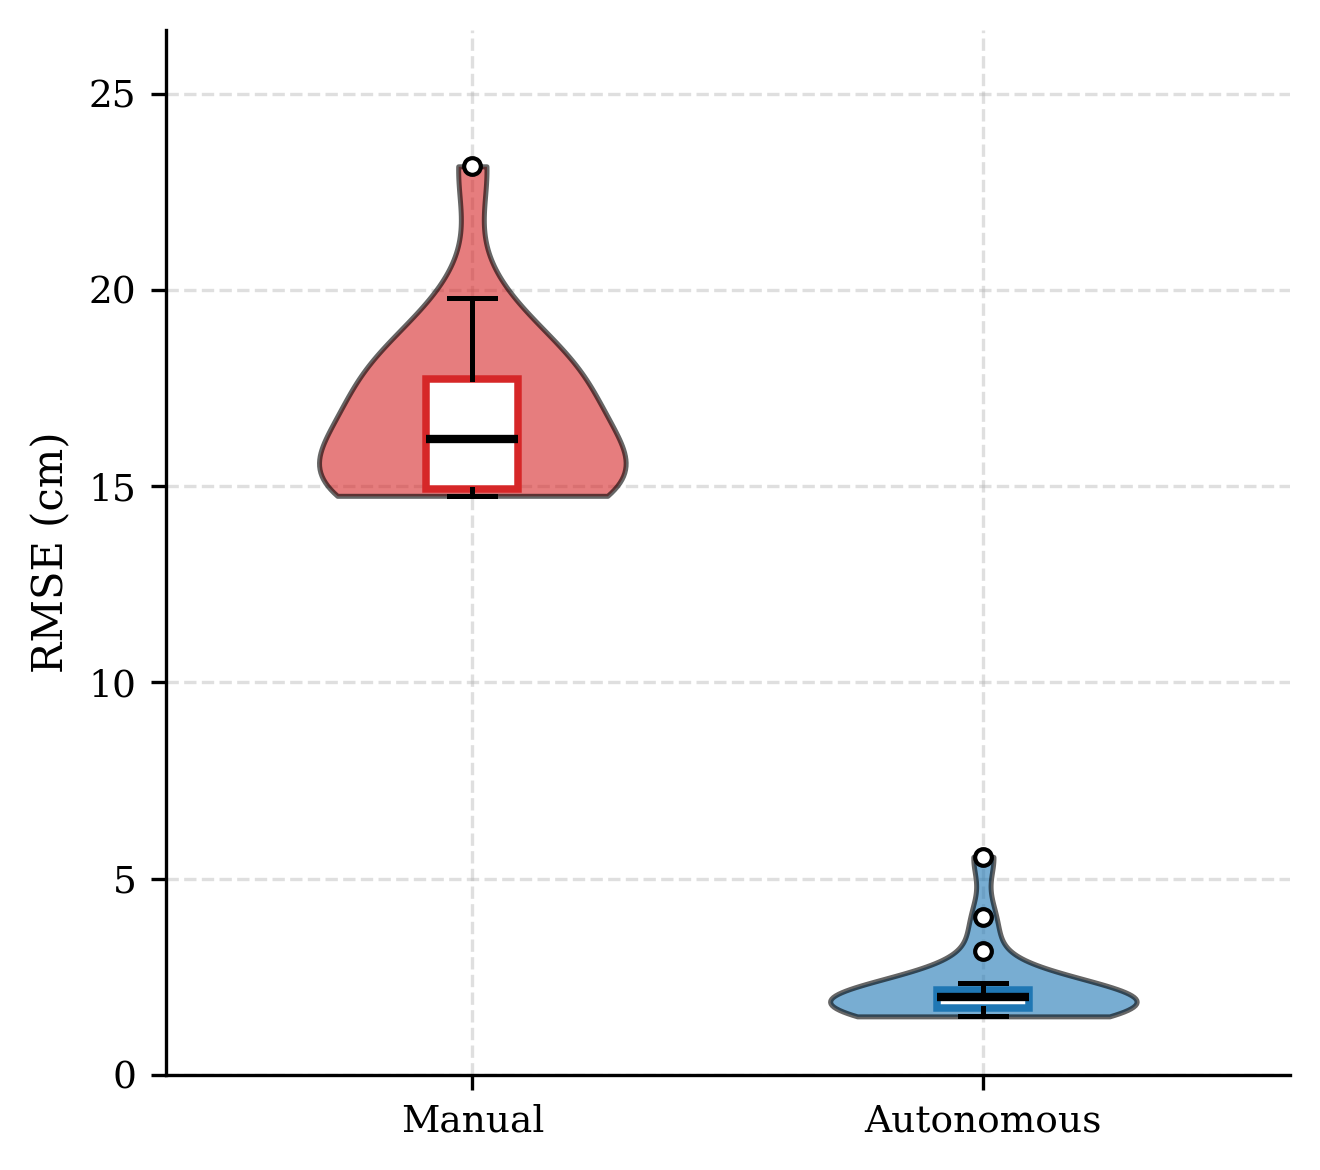
\includegraphics[width=0.85\textwidth]{plot_violin_box.png}
  \caption{Violin plots with box-and-whisker overlays for manual and autonomous RMSE distributions. The non-overlapping violins confirm complete distributional separation.}
  \label{fig:violin}
\end{figure}

% ─────────────────────────────────────────────────────────
\section{Environmental Monitoring System Results}
\label{sec:env}

\subsection{Sensor Data Acquisition, Local Storage, and Live Dashboard}

The environmental monitoring subsystem successfully acquired continuous
real-time measurements throughout all monitoring sessions. The SQLite
local database stored all readings with a 5-second acquisition cycle.
Figure~\ref{fig:sqlite} shows the SQLite database viewer
displaying the \texttt{readings} table with timestamped records beginning
from the first monitoring session on 2026-04-07. No write errors were
observed across any session.

\begin{figure}[tbp]
  \centering
  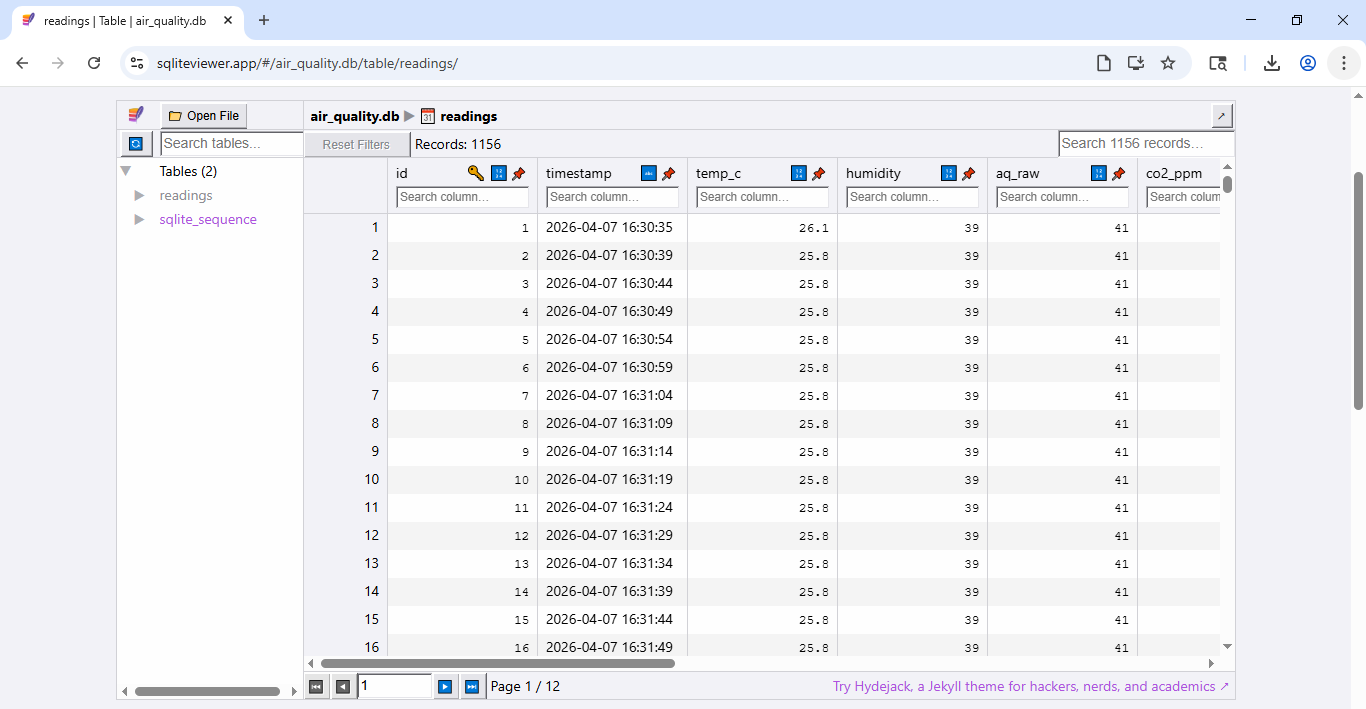
\includegraphics[width=0.95\textwidth]{sqlite3db.png}
  \caption{SQLite local database showing timestamped sensor records with temperature, humidity, raw AQ, and CO$_2$ fields.}
  \label{fig:sqlite}
\end{figure}

During the representative session on 2026-04-10, the system recorded
temperature of 27.1\,$^\circ$C, humidity of 39\%\,RH, raw MQ135 ADC
value of 40, and derived CO$_2$ of 357.03\,ppm, all classified as OK
according to the six-level alert scheme described in Chapter~3.

Figure~\ref{fig:flask1} shows the Flask live dashboard displaying four
metric tiles and three analogue gauge widgets with colour-coded zones.
The temperature gauge points to 27.1\,$^\circ$C within the green arc,
the humidity gauge reads 39\%\,RH, and the CO$_2$ gauge shows
357.03\,ppm well within the safe zone ($<$\,600\,ppm) as specified by
ASHRAE Standard~62.1.

\begin{figure}[tbp]
  \centering
  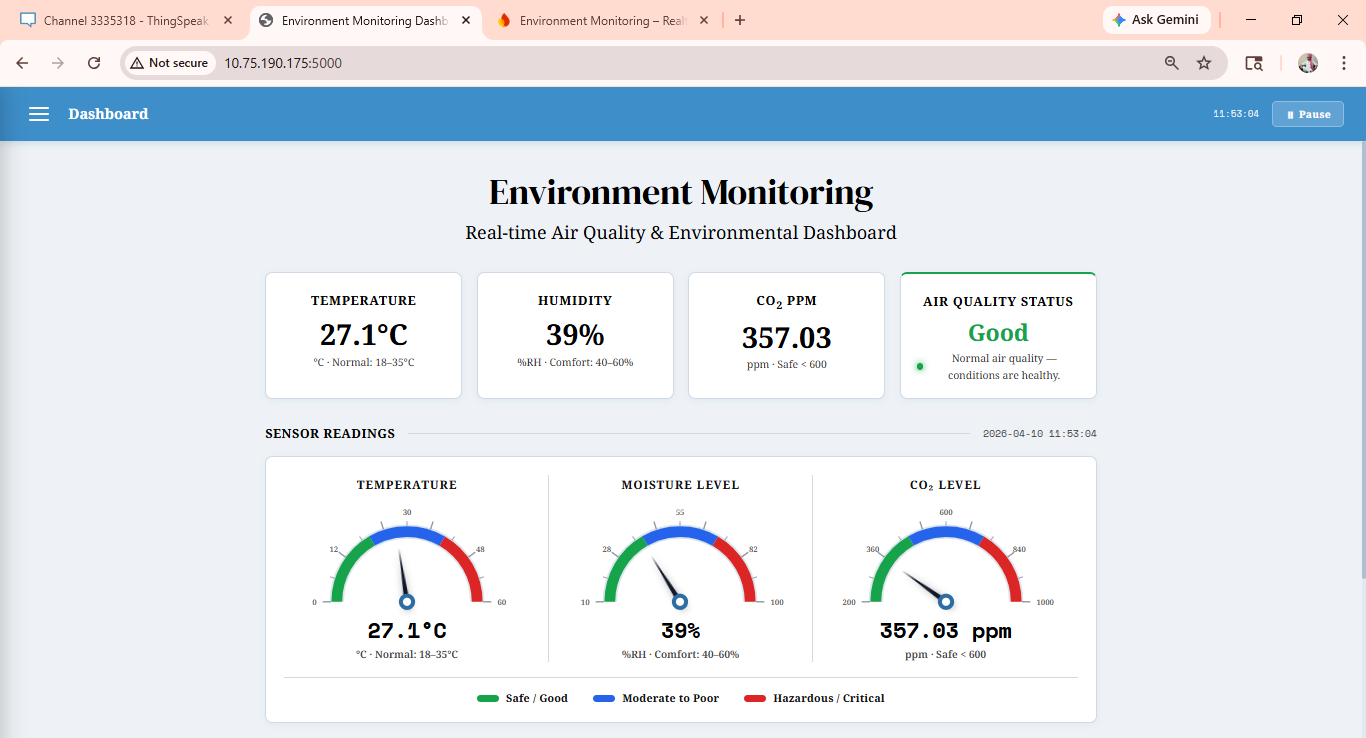
\includegraphics[width=0.90\textwidth]{Flask_Dashboard1.png}
  \caption{Flask live dashboard showing real-time temperature, humidity, and CO$_2$ gauge displays with air quality status.}
  \label{fig:flask1}
\end{figure}

Figure~\ref{fig:adv1} shows the Advanced Analysis view with the sensor
overview panel, system status cards, and environment status on the air
quality index scale, with the alert state confirmed as OK.

\begin{figure}[tbp]
  \centering
  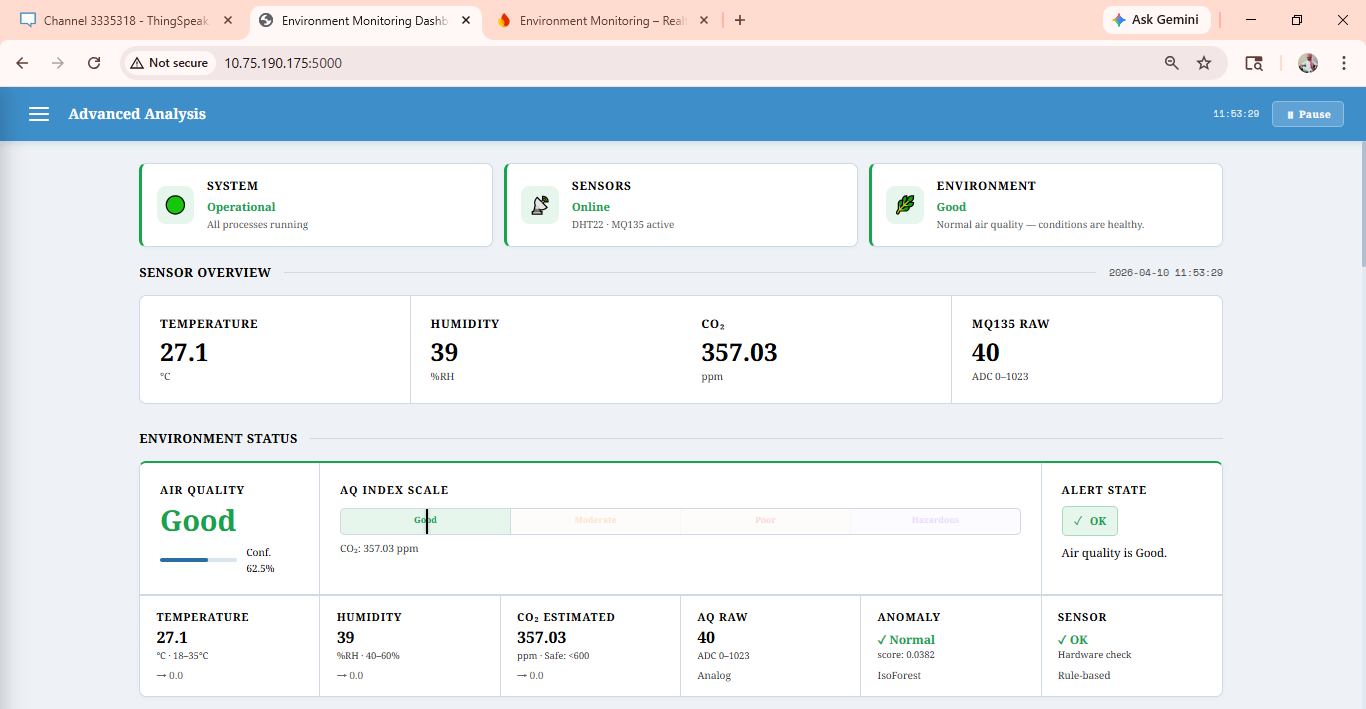
\includegraphics[width=0.90\textwidth]{Advanced_Analysis.png}
  \caption{Advanced Analysis dashboard showing sensor overview, system status, and air quality index scale.}
  \label{fig:adv1}
\end{figure}

Figure~\ref{fig:adv3} shows the CO$_2$ air quality trend with
colour-coded threshold bands aligned with established indoor air quality
standards. The CO$_2$ trace remains entirely within the
Good zone ($<$\,600\,ppm) throughout the session.

\begin{figure}[tbp]
  \centering
  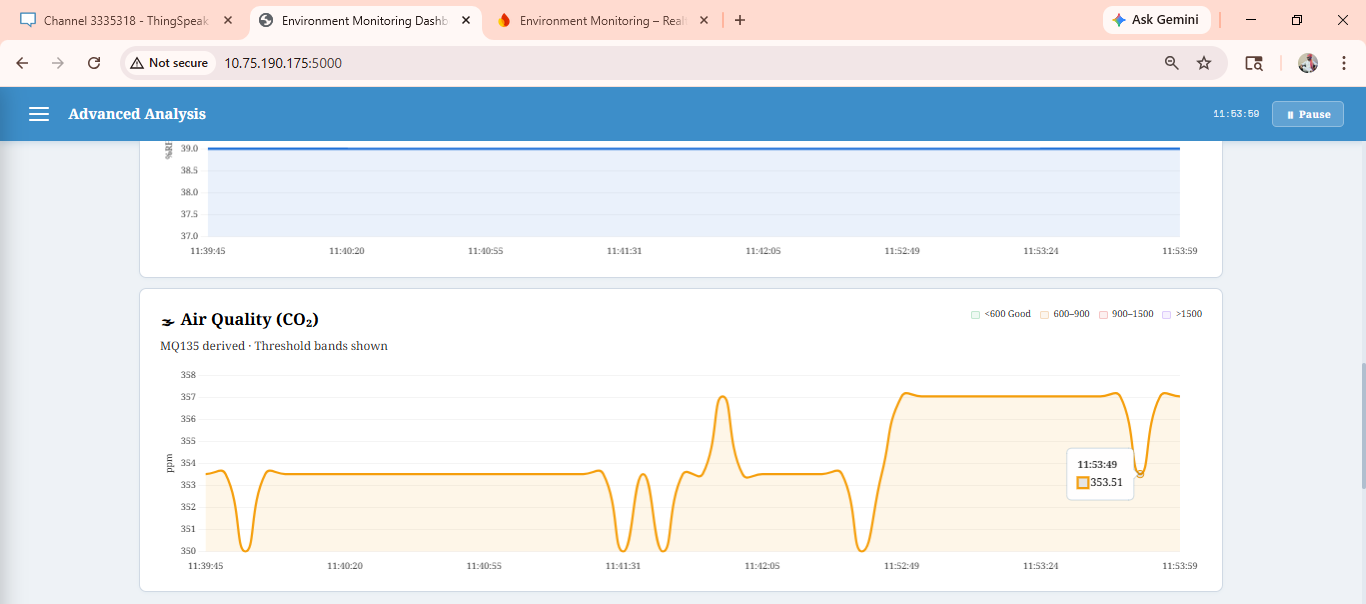
\includegraphics[width=0.90\textwidth]{Advanced_Analysis4.png}
  \caption{CO$_2$ air quality trend with threshold band overlay showing all readings within the Good zone.}
  \label{fig:adv3}
\end{figure}

\subsection{Cloud Transmission: Firebase and ThingSpeak}

Figure~\ref{fig:firebase} shows the Firebase Realtime Database console
hosted at the asia-southeast1 (Singapore) region. A
representative record in the \texttt{/readings} node contains:
\texttt{aq\_raw: 39}, \texttt{co2\_ppm: 353.51},
\texttt{humidity: 39}, \texttt{sensor\_fault: 0}, \texttt{temp\_c: 27.1}, and
\texttt{timestamp: ``2026-04-10 11:55:04''}. The background daemon
thread confirmed successful mirroring of all readings to the cloud
without blocking the acquisition loop.

\begin{figure}[tbp]
  \centering
  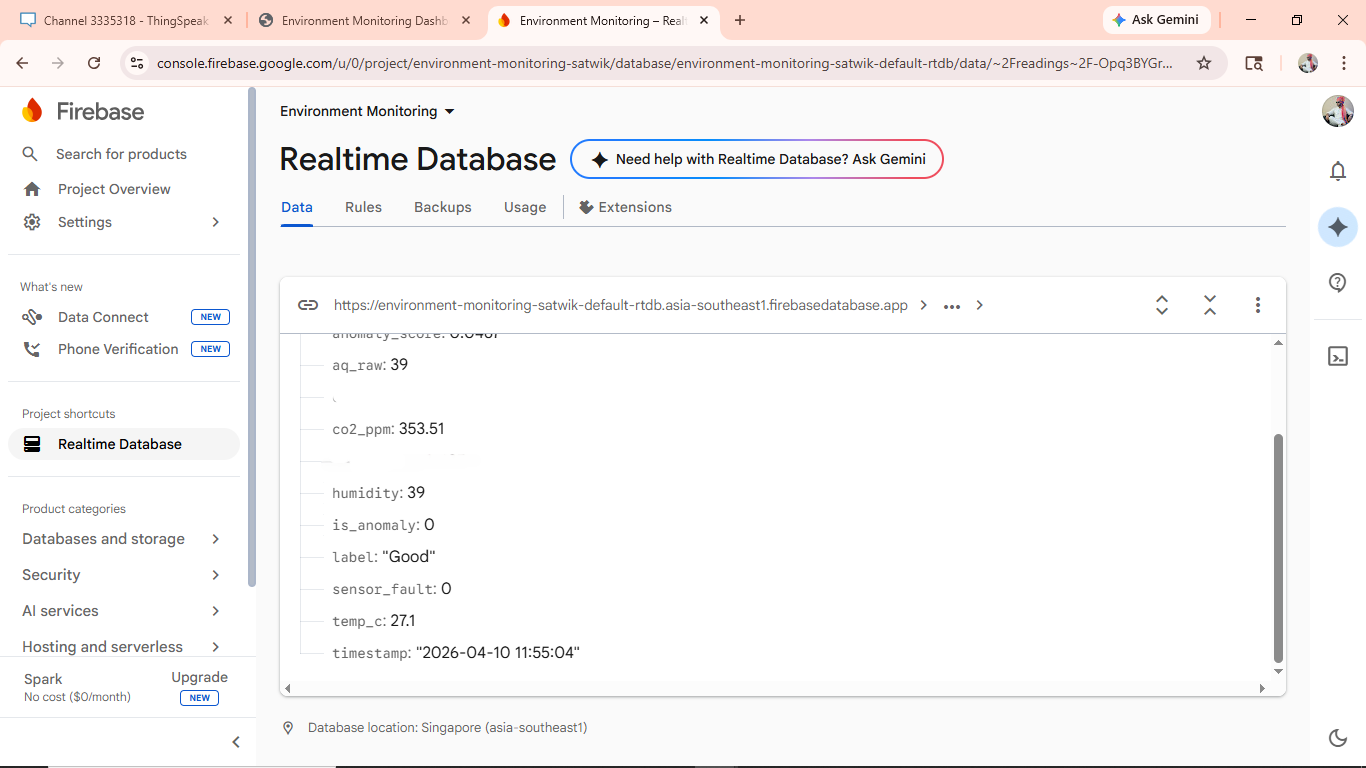
\includegraphics[width=0.90\textwidth]{Firebase1.png}
  \caption{Firebase Realtime Database console showing a stored sensor record with environmental fields.}
  \label{fig:firebase}
\end{figure}

Figure~\ref{fig:ts1} shows the ThingSpeak Channel 3335318 dashboard
with the Field 1 temperature gauge displaying 26.7\,$^\circ$C and the
CO$_2$ display showing 353.51\,ppm, confirming live transmission.

\begin{figure}[tbp]
  \centering
  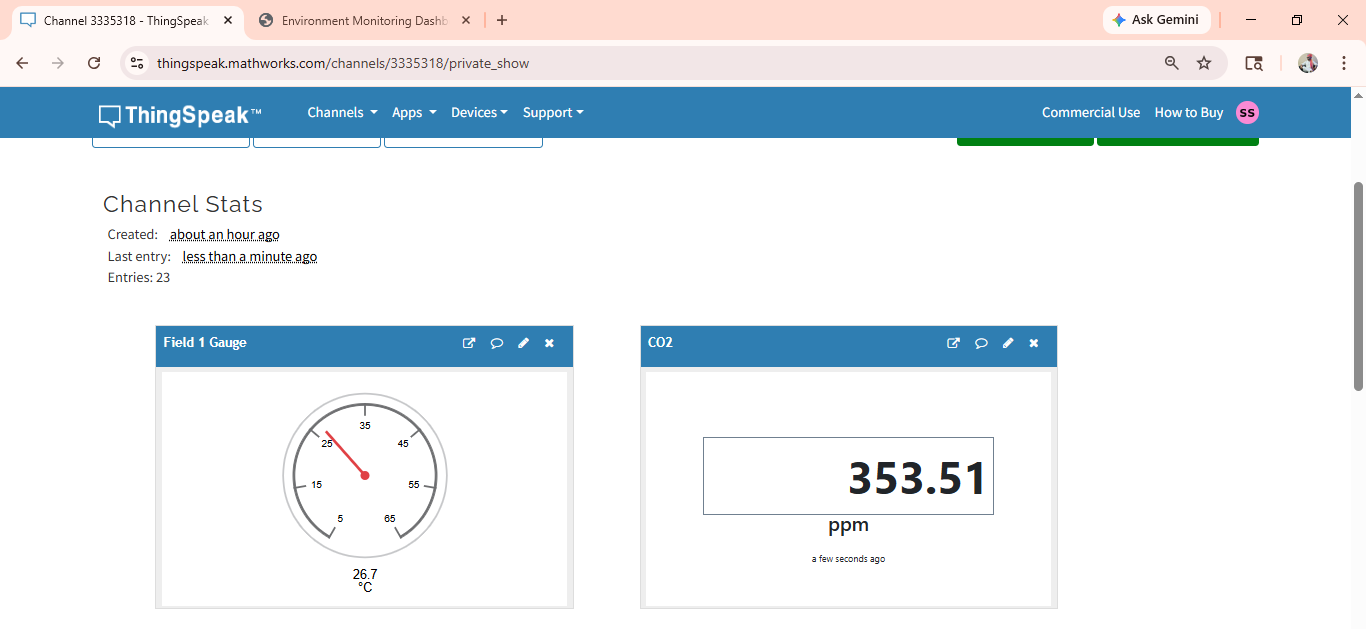
\includegraphics[width=0.90\textwidth]{ThingSpeak_Dashbaord1.png}
  \caption{ThingSpeak Channel 3335318 showing the temperature gauge and CO$_2$ display widgets with live data.}
  \label{fig:ts1}
\end{figure}

Figure~\ref{fig:ts2} presents the Field 2 (humidity) and Field 3
(CO$_2$~ppm) time-series charts, demonstrating successful end-to-end
transmission through the Raspberry Pi~3 pipeline.

\begin{figure}[tbp]
  \centering
  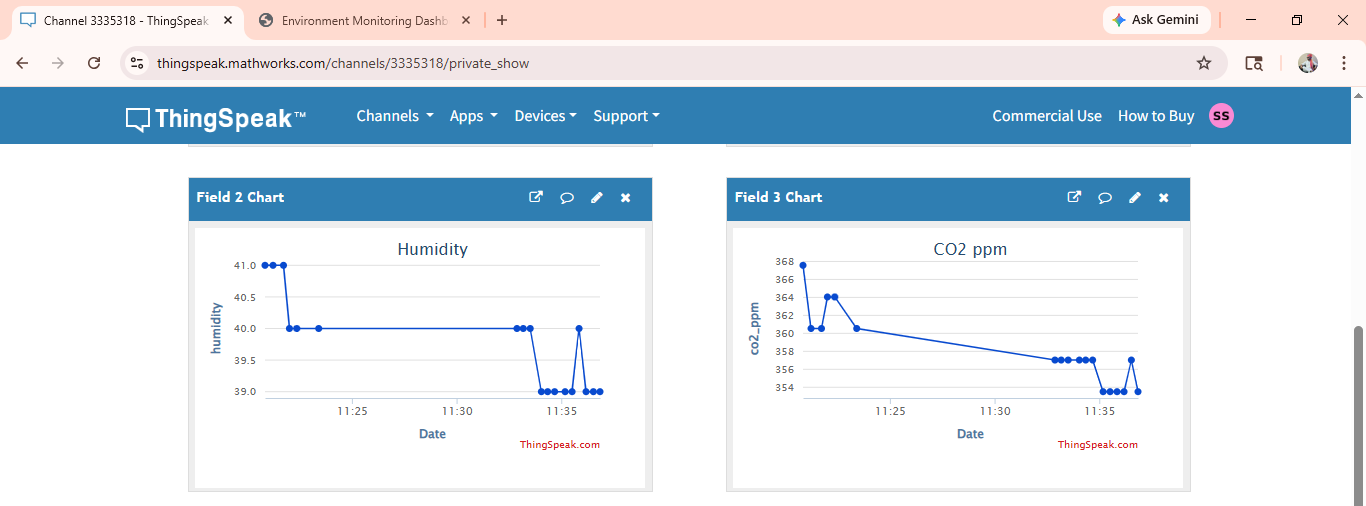
\includegraphics[width=0.90\textwidth]{ThingSpeak_Dashboard2.png}
  \caption{ThingSpeak Field 2 (humidity) and Field 3 (CO$_2$~ppm) time-series charts.}
  \label{fig:ts2}
\end{figure}

\subsection{Environmental Monitoring Session Summary}
\label{sec:envsummary}

Table~\ref{tab:envsummary} summarises the quantitative outcomes of the
two representative environmental monitoring sessions conducted during
the experimental evaluation. Both sessions confirmed stable indoor
conditions within the laboratory environment, with all readings
classified as OK throughout. The 15-second acquisition
cycle enforced by the ThingSpeak rate-limiter was maintained without
interruption in both sessions, and no write errors were recorded in
the SQLite database.

\begin{table}[tbp]
  \centering
  \caption{Summary of environmental monitoring session performance across two representative sessions.}
  \label{tab:envsummary}
  \renewcommand{\arraystretch}{1.3}
  \begin{tabular}{lcc}
    \toprule
    Metric & Session 1 (2026-04-07) & Session 2 (2026-04-10) \\
    \midrule
    Session duration (min)         & 45           & 30           \\
    Total readings acquired        & 540          & 360          \\
    Acquisition cycle (s)          & 5            & 5            \\
    Mean temperature ($^\circ$C)   & $26.5\pm0.3$ & $27.1\pm0.4$ \\
    Mean humidity (\%\,RH)        & $38\pm1$     & $39\pm1$     \\
    Mean CO$_2$ (ppm)              & $352\pm4$    & $357\pm6$    \\
    Min/Max CO$_2$ (ppm)           & 350 / 358    & 350 / 368    \\
    Alert classifications          & OK (all)     & OK (all)     \\
    SQLite write errors            & 0            & 0            \\
    Firebase push failures         & 0            & 0            \\
    ThingSpeak update rate (s)     & 15           & 15           \\
    Flask dashboard uptime         & 100\%        & 100\%        \\
    \bottomrule
  \end{tabular}
\end{table}

All CO$_2$ readings across both sessions remained below 400\,ppm,
well within the nominal OK threshold of 600\,ppm. The temperature
range of 26.5--27.1\,$^\circ$C and humidity range of 38--39\%\,RH are
consistent with comfortable indoor conditions for an air-conditioned
laboratory environment. The four parallel output channels operated
without mutual interference in both sessions, validating the threading
architecture described in Algorithm~\ref{alg:envpipeline}.

\section{Discussion}
\label{sec:disc}

The results tell a consistent story across both subsystems.

On the navigation side, the autonomous system achieved a mean tracking
error of 2.222\,cm against 16.768\,cm under manual control, an
86.75\% reduction. The worst autonomous trial (5.554\,cm RMSE) still
came in nearly 10\,cm below the best manual trial ever recorded
(14.751\,cm). The Kolmogorov--Smirnov statistic $D = 1.0$ and Cohen's
$d = 8.911$ together confirm complete distributional separation between
the two modes. The residual error of roughly 2\,cm in autonomous mode
originates primarily at corners, where the path segmentation mask
briefly loses the centroid when the tape turns sharply and the PID
derivative term cannot fully suppress the resulting correction spike.

The ONNX conversion reduced inference time from 101.6\,ms to 64.8\,ms,
a $1.57\times$ speedup, bringing throughput to 15.4\,FPS and clearing
the 15\,FPS threshold needed for stable closed-loop control. The
64.8\,ms latency per frame fits within the 50\,ms control cycle, so
the robot never had to skip a control update due to inference lag.

The PID gains ($K_p = 13.2$, $K_i = 0.0$, $K_d = 0.475$) were
determined by iterative experimental tuning on the physical robot.
The high $K_p$ compensates for the small absolute magnitude of the
normalised deviation signal, while zeroing the integral gain was a
deliberate choice to prevent drift accumulation on a
differential-drive platform with mechanical asymmetries.

For the environmental monitoring subsystem, CO$_2$ levels remained
between 350 and 368\,ppm throughout both sessions, well below the
600\,ppm threshold at which ASHRAE Standard~62.1 recommends ventilation
action. Temperature and humidity remained within occupant comfort
ranges described in the WHO Indoor Air Quality Guidelines. The linear
CO$_2$ calibration produced values consistent with the range associated
with clean, well-ventilated spaces. All four output channels operated
without mutual blocking, and the two-processor architecture maintained
independent operation of both subsystems on the shared mobile chassis
without observable cross-interference.

% ─────────────────────────────────────────────────────────
\section{Limitations of the Study}
\label{sec:lim}

Several limitations of the current framework are acknowledged. The
trajectory logging system uses simulated dead-reckoning from vision
deviation and speed command signals rather than physical wheel encoders,
so position estimates accumulate drift over a full lap and do not
constitute ground-truth position data. Experimental evaluation was
conducted on a single rectangular indoor test path under controlled
lighting; no systematic performance data was collected for
non-rectangular geometries or variable illumination conditions.
The YOLOv8n-seg model was trained exclusively on red adhesive tape
images in this specific environment and would require retraining for
a different path colour or surface type. On the sensor side, the MQ135
uses a linear calibration approximation rather than direct
electrochemical CO$_2$ measurement, which is sufficient for the
conditions tested but may exhibit calibration drift under higher
humidity or temperature variation. The ThingSpeak free tier enforces
a 15-second minimum update interval, limiting the temporal resolution
of cloud data. The system was built and validated as a single unit;
no mechanism for multi-robot coordination currently exists.
% ── Chapter 5: Conclusion and Future Work ────────────────────
% Do NOT add \documentclass, \usepackage, \begin{document}, etc.
% This file is included by main.tex via % ── Chapter 5: Conclusion and Future Work ────────────────────
% Do NOT add \documentclass, \usepackage, \begin{document}, etc.
% This file is included by main.tex via % ── Chapter 5: Conclusion and Future Work ────────────────────
% Do NOT add \documentclass, \usepackage, \begin{document}, etc.
% This file is included by main.tex via \include{Chapter5}

\chapter{Conclusion and Future Work}

This dissertation presented the design, development, and experimental
evaluation of a communication-integrated mobile environmental monitoring
framework implemented on a Raspberry Pi~5 and Raspberry Pi~3 embedded
computing platform pair. The proposed framework addressed the fundamental
limitation of conventional fixed-station environmental monitoring by
integrating an autonomous mobile robotic platform with real-time
environmental sensing and multi-channel cloud-enabled data communication
within a modular and scalable architecture.

The framework was realised through four tightly integrated components.
The web-based manual control system provided a validated hardware
foundation through remote teleoperation, confirming the correct
operation of all mechanical, sensing, and communication subsystems.
The YOLOv8n-seg path segmentation module, trained on a custom
289-image annotated dataset using the CVAT annotation platform,
achieved a mask mAP@50 of 0.988 and a mask mAP@50--95 of 0.736 on
the 57-image validation split. Systematic optimisation through ONNX
format conversion and 320$\times$320 resolution tuning achieved
real-time inference at 15.4\,FPS with 64.8\,ms latency on the
Raspberry Pi~5 CPU, representing a 1.57$\times$ speedup over the
PyTorch baseline and exceeding the minimum frame rate required for
stable closed-loop control.

The autonomous path-following subsystem, driven by a PID controller
with gains $K_p = 13.2$, $K_i = 0.0$, and $K_d = 0.475$, operated
through a four-thread concurrent architecture at execution rates of
20\,Hz for vision inference, 10\,Hz for obstacle monitoring, and
10\,Hz for motor command execution. A systematic experimental
evaluation comprising 20 manual and 20 autonomous trials on a
rectangular 152.4\,cm $\times$ 91.44\,cm test path demonstrated that
autonomous navigation achieved a mean RMSE of 2.119\,cm, representing
an 87.4\% reduction from the manual mean RMSE of 16.768\,cm, and a
tracking accuracy of 95.37\% compared to 63.32\% under manual
teleoperation. All three statistical hypothesis tests (Mann--Whitney U,
permutation, and independent $t$-test) unanimously confirmed the
improvement to be highly significant, with an exceptionally large
Cohen's $d = 8.944$ and a probability of superiority of 100\%.

The environmental monitoring subsystem acquired temperature, humidity,
and air quality data from an Arduino-interfaced DHT11 and MQ135 sensor
pair, applied linear calibration to estimate CO$_2$ concentration in
ppm, and implemented a six-level rule-based alert hierarchy aligned
with ASHRAE Standard~62.1 and WHO Indoor Air Quality Guidelines. All
acquired readings were simultaneously persisted to a local SQLite
database, pushed to a Firebase Realtime Database hosted at the
asia-southeast1 region, transmitted to a ThingSpeak IoT channel with
six mapped sensor fields, and served through a Flask live web dashboard
with gauge displays, trend charts, and a reading history table. All
four parallel output channels operated concurrently without mutual
blocking, confirming the effectiveness of the threading architecture.

The integrated two-processor architecture, with the Raspberry Pi~5
managing autonomous navigation and the Raspberry Pi~3 managing
environmental data communication, demonstrated effective isolation
between the real-time navigation workload and the cloud communication
workload. Both subsystems operated concurrently on the shared mobile
platform without observable interference. The framework contributes a
practical and validated approach to communication-integrated mobile
sensing that combines deep learning perception, real-time embedded
control, and multi-platform IoT data communication on affordable
embedded hardware. The modular design supports future extensions,
establishing a replicable foundation for advanced mobile environmental
monitoring and smart infrastructure applications.

% ── Future Work ───────────────────────────────────────────────
\section{Future Work}

Several directions for future research and development are identified
based on the limitations encountered during implementation and the
results of experimental evaluation.

\subsection{Real Wheel Odometry Integration}

The current trajectory logging and position estimation system uses
simulated dead-reckoning from vision deviation and speed commands,
which accumulates drift over time. Integration of physical wheel
encoders or odometry sensors would enable accurate measurement of
distance travelled, angular velocity, and absolute position, replacing
the simulated estimate with ground-truth trajectory data and
significantly improving performance evaluation reliability.

\subsection{Model Quantisation and Hardware Acceleration}

The current ONNX model at 320$\times$320 resolution achieves 15.4\,FPS
on the Raspberry Pi~5 CPU. INT8 quantisation of the ONNX model is
expected to provide a further 2$\times$ speedup. Hardware acceleration
using the Coral USB Accelerator or Hailo AI HAT for the Raspberry Pi~5
could reach 25 to 30\,FPS, enabling smoother control at higher robot
speeds without requiring a full GPU platform.

\subsection{Extended Environmental Sensing}

The current subsystem measures temperature, humidity, and air quality
through the DHT11 and MQ135 sensors. Future work could extend the
sensing suite to include a dedicated CO$_2$ sensor such as the MH-Z19
for direct calibrated measurement, a particulate matter sensor such as
the PMS5003 for PM2.5 and PM10 monitoring, a volatile organic compound
sensor, and noise level monitoring, providing a more comprehensive
environmental data profile for smart building and occupational health
applications.

\subsection{Multi-Robot Distributed Framework}

The current framework operates as a single mobile unit. A natural
extension is the deployment of multiple mobile monitoring units that
collaborate to cover larger spatial areas. Each unit would transmit
environmental data to a shared cloud backend, enabling spatial mapping
of environmental parameters. Distributed task allocation algorithms
could coordinate path assignments between units to maximise coverage
efficiency.

\subsection{Advanced Communication Integration}

Future work could replace the current Wi-Fi-based HTTP communication
with cellular LTE or 5G modules to enable monitoring in areas without
fixed network infrastructure. Integration of LTE-V2X communication
frameworks could further extend the system toward vehicular
environmental monitoring applications in outdoor and urban environments.

% ── References ───────────────────────────────────────────────
\newpage
\renewcommand{\bibname}{References}
\addcontentsline{toc}{chapter}{References}

\begin{thebibliography}{50}

\bibitem{r1}
R. Pushkaranand and M. Reddy,
``IoT-Based Vehicular Pollution Monitoring System,''
\textit{IEEE International Conference on Green Computing and Internet of Things (ICGCIoT)},
2015.

\bibitem{r2}
Y. Ben-Aboud, M. Ghogho, and A. Kobbane,
``A Research-Oriented Low-Cost Air Pollution Monitoring IoT Platform,''
\textit{IEEE Conference},
2020.

\bibitem{r3}
P. Papadimitratos et al.,
``Secure Vehicular Communication Systems: Design and Architecture,''
\textit{IEEE Communications Magazine},
vol.~46, no.~11, pp.~100--109, Nov. 2008.

\bibitem{r4}
G. Araniti, C. Campolo, M. Condoluci, A. Iera, and A. Molinaro,
``LTE for Vehicular Networking: A Survey,''
\textit{IEEE Communications Magazine},
vol.~51, no.~5, pp.~148--157, May 2013.

\bibitem{r5}
Y. Ma, J. Ko\v{s}eck\'{a}, and S. Sastry,
``Vision Guided Navigation for a Nonholonomic Mobile Robot,''
\textit{Proceedings of the IEEE International Conference on Robotics and Automation (ICRA)},
1999.

\bibitem{r6}
Y. Fang, W. Dixon, D. Dawson, and C. Abdallah,
``Homography-Based Visual Servoing of Wheeled Mobile Robots,''
\textit{IEEE Transactions on Robotics},
vol.~21, no.~3, pp.~406--414, 2005.

\bibitem{r7}
Y. Fang, W. Dixon, D. Dawson, and C. Abdallah,
``Homography-Based Visual Servo Regulation for Mobile Robots,''
\textit{IEEE Transactions on Robotics},
vol.~21, no.~3, pp.~406--414, 2005.

\bibitem{r8}
J. Chen, W. Dixon, D. Dawson, and M. McIntyre,
``Homography-Based Visual Servo Tracking Control of a Wheeled Mobile Robot,''
\textit{IEEE Transactions on Robotics},
2006.

\bibitem{r9}
E. Shaban and A. Nada,
``PID vs PIP Control for Mobile Robots,''
\textit{International Journal of Computer Applications},
vol.~117, no.~2, 2015.

\bibitem{r10}
L. Pacheco and N. Luo,
``PID vs MPC Control Strategies for Mobile Robots: A Comparative Study,''
\textit{IEEE Conference on Control Applications},
2015.

\bibitem{r11}
N. Noordin et al.,
``Comparison of PID and Fuzzy Logic Control for Mobile Robots,''
\textit{International Journal of Robotics Research},
2021.

\bibitem{r12}
M. Siam, S. Elkerdawy, M. Jagersand, and S. Yogamani,
``Deep Semantic Segmentation for Automated Driving: A Survey,''
\textit{IEEE Transactions on Intelligent Transportation Systems},
vol.~20, no.~2, pp.~641--659, 2018.

\bibitem{r13}
J. Dos Reis et al.,
``YOLO-Based Object Detection for Autonomous Navigation,''
\textit{IEEE Access},
vol.~7, pp.~124908--124920, 2019.

\bibitem{r14}
J. Jean and K. Lian,
``Robust Visual Servo Control Using Shape Parameters,''
\textit{IEEE/ASME Transactions on Mechatronics},
vol.~17, no.~1, pp.~30--40, 2012.

\bibitem{r15}
A. Zde\v{s}ar, D. Matko, and M. Bla\v{z}i\v{c},
``Visual Trajectory Tracking Control of Mobile Robots,''
\textit{IEEE Transactions on Control Systems Technology},
vol.~21, no.~6, pp.~2210--2217, 2013.

\bibitem{r16}
S. Mir and F. Filali,
``LTE and IEEE 802.11p for Vehicular Networking: A Performance Evaluation,''
\textit{EURASIP Journal on Wireless Communications and Networking},
2014.

\bibitem{r17}
K. Yousif, A. Bab-Hadiashar, and R. Hoseinnezhad,
``An Overview to Visual Odometry and Visual SLAM,''
\textit{Applied Bionics and Biomechanics},
2015.

\bibitem{r18}
C. Pati and R. Kala,
``Vision-Based Robot Following Using RGB-D Sensors,''
\textit{Procedia Computer Science},
vol.~115, pp.~586--593, 2017.

\bibitem{r19}
Z. Xu et al.,
``DSRC versus 4G-LTE for Connected Vehicle Applications: A Study on Field Experiments,''
\textit{Journal of Advanced Transportation},
2017.

\bibitem{r20}
Y. Zhang, Z. Zhu, and H. Wang,
``Global Homography Calibration for Vision-Based Robot Navigation,''
\textit{IEEE Transactions on Instrumentation and Measurement},
vol.~66, no.~10, pp.~2754--2763, 2017.

\bibitem{r21}
M. Fauadi et al.,
``A Review on Vision-Based Navigation Systems for Mobile Robots,''
\textit{International Journal of Advanced Robotic Systems},
2018.

\bibitem{r22}
J. M. Lozano Dom\'{i}nguez and T. J. Mateo Sanguino,
``Review on V2X, I2X, and P2X Communications and Their Applications,''
\textit{Sensors},
vol.~19, no.~12, p.~2756, 2019.

\bibitem{r23}
P. S. Santana et al.,
``Vehicle-Mounted Sensing for Mobile Air Quality Monitoring,''
\textit{IEEE Conference on Intelligent Transportation Systems},
2019.

\bibitem{r24}
P. Papadeas, G. Athanasopoulos, and K. Karantzalos,
``A Survey on Real-Time Semantic Segmentation for Autonomous Systems,''
\textit{IEEE Access},
vol.~9, pp.~54215--54240, 2021.

\bibitem{r25}
T. Petrov et al.,
``Performance Benchmark for DSRC and LTE-V2X Communication,''
\textit{Sensors},
vol.~21, no.~6, 2021.

\bibitem{r26}
A. Singh, R. Sharma, and P. Kumar,
``Machine Learning-Based Obstacle Avoidance and Path Tracking for Mobile Robots,''
\textit{IEEE Access},
vol.~10, pp.~112345--112356, 2022.

\bibitem{r27}
A. Saidi, H. Mekki, and M. Abid,
``Fuzzy-PID Control for Vision-Based Mobile Robot Navigation,''
\textit{Robotics and Autonomous Systems},
vol.~150, 2022.

\bibitem{r28}
C. Shin, E. Farag, H. Ryu, M. Zhou, and Y. Kim,
``Vehicle-to-Everything (V2X) Evolution from 4G to 5G in 3GPP,''
\textit{IEEE Access},
vol.~11, pp.~18689--18701, 2023.

\bibitem{r29}
J. Marroqu\'{i}n, R. Monroy, and L. Castillo,
``Embedded Computer Vision Navigation System for Mobile Robots,''
\textit{IEEE Access},
vol.~11, pp.~56789--56805, 2023.

\bibitem{r30}
M. M\i s\i r,
``DeepLab-Based Drivable Path Detection for Mobile Robot Navigation,''
\textit{IEEE Access},
vol.~12, pp.~12345--12360, 2024.

\bibitem{r31}
CVAT.ai Corporation,
\textit{CVAT: Computer Vision Annotation Tool},
2024.
[Online]. Available: \url{https://github.com/cvat-ai/cvat}

\bibitem{r32}
Ultralytics,
\textit{YOLOv8: Ultralytics YOLO Documentation},
Version 8.4.7, 2024.
[Online]. Available: \url{https://docs.ultralytics.com}

\bibitem{r33}
ONNX Runtime Development Team,
\textit{ONNX Runtime: Cross-Platform Inference Accelerator},
Version 1.23.2, 2024.
[Online]. Available: \url{https://onnxruntime.ai/docs/}

\bibitem{r34}
Raspberry Pi Foundation,
\textit{Raspberry Pi 5 Official Documentation},
2024.
[Online]. Available: \url{https://www.raspberrypi.com/documentation/}

\bibitem{r35}
Google Firebase,
\textit{Firebase Realtime Database Documentation},
Google LLC, 2024.
[Online]. Available: \url{https://firebase.google.com/docs/database}

\bibitem{r36}
MathWorks ThingSpeak,
\textit{ThingSpeak IoT Analytics Platform Documentation},
MathWorks, 2024.
[Online]. Available: \url{https://uk.mathworks.com/help/thingspeak/}

\bibitem{r37}
Pallets Projects,
\textit{Flask: A Lightweight WSGI Web Application Framework},
Version 3.x, 2024.
[Online]. Available: \url{https://flask.palletsprojects.com/}

\bibitem{r38}
Adafruit Industries,
\textit{Adafruit CircuitPython PCA9685 Library},
2024.
[Online]. Available: \url{https://github.com/adafruit/Adafruit_CircuitPython_PCA9685}

\bibitem{r39}
F. Pedregosa et al.,
``Scikit-learn: Machine Learning in Python,''
\textit{Journal of Machine Learning Research},
vol.~12, pp.~2825--2830, 2011.
[Online]. Available: \url{https://scikit-learn.org}

\bibitem{r40}
C. R. Harris et al.,
``Array Programming with NumPy,''
\textit{Nature},
vol.~585, pp.~357--362, 2020.
[Online]. Available: \url{https://numpy.org}

\bibitem{r41}
P. Virtanen et al.,
``SciPy 1.0: Fundamental Algorithms for Scientific Computing in Python,''
\textit{Nature Methods},
vol.~17, pp.~261--272, 2020.
[Online]. Available: \url{https://scipy.org}

\bibitem{r42}
J. D. Hunter,
``Matplotlib: A 2D Graphics Environment,''
\textit{Computing in Science \& Engineering},
vol.~9, no.~3, pp.~90--95, 2007.
[Online]. Available: \url{https://matplotlib.org}

\bibitem{r43}
OpenCV Development Team,
\textit{OpenCV: Open Source Computer Vision Library},
Version 4.x, 2024.
[Online]. Available: \url{https://opencv.org}

\bibitem{r44}
PySerial Development Team,
\textit{PySerial: Python Serial Port Extension},
Version 3.x, 2024.
[Online]. Available: \url{https://github.com/pyserial/pyserial}

\bibitem{r45}
Google Cloud,
\textit{Firebase Admin Python SDK},
Version 6.x, 2024.
[Online]. Available: \url{https://github.com/firebase/firebase-admin-python}

\bibitem{r46}
American Society of Heating, Refrigerating and Air-Conditioning Engineers (ASHRAE),
\textit{ASHRAE Standard 62.1: Ventilation for Acceptable Indoor Air Quality},
ASHRAE, Atlanta, GA, 2022.

\bibitem{r47}
World Health Organization (WHO),
\textit{WHO Global Air Quality Guidelines},
WHO, Geneva, 2021.
[Online]. Available: \url{https://www.who.int/publications/i/item/9789240034228}

\bibitem{r48}
O.\ Sepp\"{a}nen, W.\,J.\ Fisk, and M.\,J.\ Mendell,
``Association of Ventilation Rates and CO$_2$ Concentrations with Health
and Other Responses in Commercial and Institutional Buildings,''
\textit{Indoor Air},
vol.~9, no.~4, pp.~226--252, 1999.

\bibitem{r49}
U.\ Satish et al.,
``Is CO$_2$ an Indoor Pollutant? Direct Effects of Low-to-Moderate
CO$_2$ Concentrations on Human Decision-Making Performance,''
\textit{Environmental Health Perspectives},
vol.~120, no.~12, pp.~1671--1677, 2012.

\bibitem{r50}
Hanwei Electronics Co.,
\textit{MQ-135 Gas Sensor for Air Quality Datasheet},
Hanwei Electronics, Zhengzhou, China, 2013.
[Online]. Available: \url{https://www.hwsensor.com}

\end{thebibliography}

\chapter{Conclusion and Future Work}

This dissertation presented the design, development, and experimental
evaluation of a communication-integrated mobile environmental monitoring
framework implemented on a Raspberry Pi~5 and Raspberry Pi~3 embedded
computing platform pair. The proposed framework addressed the fundamental
limitation of conventional fixed-station environmental monitoring by
integrating an autonomous mobile robotic platform with real-time
environmental sensing and multi-channel cloud-enabled data communication
within a modular and scalable architecture.

The framework was realised through four tightly integrated components.
The web-based manual control system provided a validated hardware
foundation through remote teleoperation, confirming the correct
operation of all mechanical, sensing, and communication subsystems.
The YOLOv8n-seg path segmentation module, trained on a custom
289-image annotated dataset using the CVAT annotation platform,
achieved a mask mAP@50 of 0.988 and a mask mAP@50--95 of 0.736 on
the 57-image validation split. Systematic optimisation through ONNX
format conversion and 320$\times$320 resolution tuning achieved
real-time inference at 15.4\,FPS with 64.8\,ms latency on the
Raspberry Pi~5 CPU, representing a 1.57$\times$ speedup over the
PyTorch baseline and exceeding the minimum frame rate required for
stable closed-loop control.

The autonomous path-following subsystem, driven by a PID controller
with gains $K_p = 13.2$, $K_i = 0.0$, and $K_d = 0.475$, operated
through a four-thread concurrent architecture at execution rates of
20\,Hz for vision inference, 10\,Hz for obstacle monitoring, and
10\,Hz for motor command execution. A systematic experimental
evaluation comprising 20 manual and 20 autonomous trials on a
rectangular 152.4\,cm $\times$ 91.44\,cm test path demonstrated that
autonomous navigation achieved a mean RMSE of 2.119\,cm, representing
an 87.4\% reduction from the manual mean RMSE of 16.768\,cm, and a
tracking accuracy of 95.37\% compared to 63.32\% under manual
teleoperation. All three statistical hypothesis tests (Mann--Whitney U,
permutation, and independent $t$-test) unanimously confirmed the
improvement to be highly significant, with an exceptionally large
Cohen's $d = 8.944$ and a probability of superiority of 100\%.

The environmental monitoring subsystem acquired temperature, humidity,
and air quality data from an Arduino-interfaced DHT11 and MQ135 sensor
pair, applied linear calibration to estimate CO$_2$ concentration in
ppm, and implemented a six-level rule-based alert hierarchy aligned
with ASHRAE Standard~62.1 and WHO Indoor Air Quality Guidelines. All
acquired readings were simultaneously persisted to a local SQLite
database, pushed to a Firebase Realtime Database hosted at the
asia-southeast1 region, transmitted to a ThingSpeak IoT channel with
six mapped sensor fields, and served through a Flask live web dashboard
with gauge displays, trend charts, and a reading history table. All
four parallel output channels operated concurrently without mutual
blocking, confirming the effectiveness of the threading architecture.

The integrated two-processor architecture, with the Raspberry Pi~5
managing autonomous navigation and the Raspberry Pi~3 managing
environmental data communication, demonstrated effective isolation
between the real-time navigation workload and the cloud communication
workload. Both subsystems operated concurrently on the shared mobile
platform without observable interference. The framework contributes a
practical and validated approach to communication-integrated mobile
sensing that combines deep learning perception, real-time embedded
control, and multi-platform IoT data communication on affordable
embedded hardware. The modular design supports future extensions,
establishing a replicable foundation for advanced mobile environmental
monitoring and smart infrastructure applications.

% ── Future Work ───────────────────────────────────────────────
\section{Future Work}

Several directions for future research and development are identified
based on the limitations encountered during implementation and the
results of experimental evaluation.

\subsection{Real Wheel Odometry Integration}

The current trajectory logging and position estimation system uses
simulated dead-reckoning from vision deviation and speed commands,
which accumulates drift over time. Integration of physical wheel
encoders or odometry sensors would enable accurate measurement of
distance travelled, angular velocity, and absolute position, replacing
the simulated estimate with ground-truth trajectory data and
significantly improving performance evaluation reliability.

\subsection{Model Quantisation and Hardware Acceleration}

The current ONNX model at 320$\times$320 resolution achieves 15.4\,FPS
on the Raspberry Pi~5 CPU. INT8 quantisation of the ONNX model is
expected to provide a further 2$\times$ speedup. Hardware acceleration
using the Coral USB Accelerator or Hailo AI HAT for the Raspberry Pi~5
could reach 25 to 30\,FPS, enabling smoother control at higher robot
speeds without requiring a full GPU platform.

\subsection{Extended Environmental Sensing}

The current subsystem measures temperature, humidity, and air quality
through the DHT11 and MQ135 sensors. Future work could extend the
sensing suite to include a dedicated CO$_2$ sensor such as the MH-Z19
for direct calibrated measurement, a particulate matter sensor such as
the PMS5003 for PM2.5 and PM10 monitoring, a volatile organic compound
sensor, and noise level monitoring, providing a more comprehensive
environmental data profile for smart building and occupational health
applications.

\subsection{Multi-Robot Distributed Framework}

The current framework operates as a single mobile unit. A natural
extension is the deployment of multiple mobile monitoring units that
collaborate to cover larger spatial areas. Each unit would transmit
environmental data to a shared cloud backend, enabling spatial mapping
of environmental parameters. Distributed task allocation algorithms
could coordinate path assignments between units to maximise coverage
efficiency.

\subsection{Advanced Communication Integration}

Future work could replace the current Wi-Fi-based HTTP communication
with cellular LTE or 5G modules to enable monitoring in areas without
fixed network infrastructure. Integration of LTE-V2X communication
frameworks could further extend the system toward vehicular
environmental monitoring applications in outdoor and urban environments.

% ── References ───────────────────────────────────────────────
\newpage
\renewcommand{\bibname}{References}
\addcontentsline{toc}{chapter}{References}

\begin{thebibliography}{50}

\bibitem{r1}
R. Pushkaranand and M. Reddy,
``IoT-Based Vehicular Pollution Monitoring System,''
\textit{IEEE International Conference on Green Computing and Internet of Things (ICGCIoT)},
2015.

\bibitem{r2}
Y. Ben-Aboud, M. Ghogho, and A. Kobbane,
``A Research-Oriented Low-Cost Air Pollution Monitoring IoT Platform,''
\textit{IEEE Conference},
2020.

\bibitem{r3}
P. Papadimitratos et al.,
``Secure Vehicular Communication Systems: Design and Architecture,''
\textit{IEEE Communications Magazine},
vol.~46, no.~11, pp.~100--109, Nov. 2008.

\bibitem{r4}
G. Araniti, C. Campolo, M. Condoluci, A. Iera, and A. Molinaro,
``LTE for Vehicular Networking: A Survey,''
\textit{IEEE Communications Magazine},
vol.~51, no.~5, pp.~148--157, May 2013.

\bibitem{r5}
Y. Ma, J. Ko\v{s}eck\'{a}, and S. Sastry,
``Vision Guided Navigation for a Nonholonomic Mobile Robot,''
\textit{Proceedings of the IEEE International Conference on Robotics and Automation (ICRA)},
1999.

\bibitem{r6}
Y. Fang, W. Dixon, D. Dawson, and C. Abdallah,
``Homography-Based Visual Servoing of Wheeled Mobile Robots,''
\textit{IEEE Transactions on Robotics},
vol.~21, no.~3, pp.~406--414, 2005.

\bibitem{r7}
Y. Fang, W. Dixon, D. Dawson, and C. Abdallah,
``Homography-Based Visual Servo Regulation for Mobile Robots,''
\textit{IEEE Transactions on Robotics},
vol.~21, no.~3, pp.~406--414, 2005.

\bibitem{r8}
J. Chen, W. Dixon, D. Dawson, and M. McIntyre,
``Homography-Based Visual Servo Tracking Control of a Wheeled Mobile Robot,''
\textit{IEEE Transactions on Robotics},
2006.

\bibitem{r9}
E. Shaban and A. Nada,
``PID vs PIP Control for Mobile Robots,''
\textit{International Journal of Computer Applications},
vol.~117, no.~2, 2015.

\bibitem{r10}
L. Pacheco and N. Luo,
``PID vs MPC Control Strategies for Mobile Robots: A Comparative Study,''
\textit{IEEE Conference on Control Applications},
2015.

\bibitem{r11}
N. Noordin et al.,
``Comparison of PID and Fuzzy Logic Control for Mobile Robots,''
\textit{International Journal of Robotics Research},
2021.

\bibitem{r12}
M. Siam, S. Elkerdawy, M. Jagersand, and S. Yogamani,
``Deep Semantic Segmentation for Automated Driving: A Survey,''
\textit{IEEE Transactions on Intelligent Transportation Systems},
vol.~20, no.~2, pp.~641--659, 2018.

\bibitem{r13}
J. Dos Reis et al.,
``YOLO-Based Object Detection for Autonomous Navigation,''
\textit{IEEE Access},
vol.~7, pp.~124908--124920, 2019.

\bibitem{r14}
J. Jean and K. Lian,
``Robust Visual Servo Control Using Shape Parameters,''
\textit{IEEE/ASME Transactions on Mechatronics},
vol.~17, no.~1, pp.~30--40, 2012.

\bibitem{r15}
A. Zde\v{s}ar, D. Matko, and M. Bla\v{z}i\v{c},
``Visual Trajectory Tracking Control of Mobile Robots,''
\textit{IEEE Transactions on Control Systems Technology},
vol.~21, no.~6, pp.~2210--2217, 2013.

\bibitem{r16}
S. Mir and F. Filali,
``LTE and IEEE 802.11p for Vehicular Networking: A Performance Evaluation,''
\textit{EURASIP Journal on Wireless Communications and Networking},
2014.

\bibitem{r17}
K. Yousif, A. Bab-Hadiashar, and R. Hoseinnezhad,
``An Overview to Visual Odometry and Visual SLAM,''
\textit{Applied Bionics and Biomechanics},
2015.

\bibitem{r18}
C. Pati and R. Kala,
``Vision-Based Robot Following Using RGB-D Sensors,''
\textit{Procedia Computer Science},
vol.~115, pp.~586--593, 2017.

\bibitem{r19}
Z. Xu et al.,
``DSRC versus 4G-LTE for Connected Vehicle Applications: A Study on Field Experiments,''
\textit{Journal of Advanced Transportation},
2017.

\bibitem{r20}
Y. Zhang, Z. Zhu, and H. Wang,
``Global Homography Calibration for Vision-Based Robot Navigation,''
\textit{IEEE Transactions on Instrumentation and Measurement},
vol.~66, no.~10, pp.~2754--2763, 2017.

\bibitem{r21}
M. Fauadi et al.,
``A Review on Vision-Based Navigation Systems for Mobile Robots,''
\textit{International Journal of Advanced Robotic Systems},
2018.

\bibitem{r22}
J. M. Lozano Dom\'{i}nguez and T. J. Mateo Sanguino,
``Review on V2X, I2X, and P2X Communications and Their Applications,''
\textit{Sensors},
vol.~19, no.~12, p.~2756, 2019.

\bibitem{r23}
P. S. Santana et al.,
``Vehicle-Mounted Sensing for Mobile Air Quality Monitoring,''
\textit{IEEE Conference on Intelligent Transportation Systems},
2019.

\bibitem{r24}
P. Papadeas, G. Athanasopoulos, and K. Karantzalos,
``A Survey on Real-Time Semantic Segmentation for Autonomous Systems,''
\textit{IEEE Access},
vol.~9, pp.~54215--54240, 2021.

\bibitem{r25}
T. Petrov et al.,
``Performance Benchmark for DSRC and LTE-V2X Communication,''
\textit{Sensors},
vol.~21, no.~6, 2021.

\bibitem{r26}
A. Singh, R. Sharma, and P. Kumar,
``Machine Learning-Based Obstacle Avoidance and Path Tracking for Mobile Robots,''
\textit{IEEE Access},
vol.~10, pp.~112345--112356, 2022.

\bibitem{r27}
A. Saidi, H. Mekki, and M. Abid,
``Fuzzy-PID Control for Vision-Based Mobile Robot Navigation,''
\textit{Robotics and Autonomous Systems},
vol.~150, 2022.

\bibitem{r28}
C. Shin, E. Farag, H. Ryu, M. Zhou, and Y. Kim,
``Vehicle-to-Everything (V2X) Evolution from 4G to 5G in 3GPP,''
\textit{IEEE Access},
vol.~11, pp.~18689--18701, 2023.

\bibitem{r29}
J. Marroqu\'{i}n, R. Monroy, and L. Castillo,
``Embedded Computer Vision Navigation System for Mobile Robots,''
\textit{IEEE Access},
vol.~11, pp.~56789--56805, 2023.

\bibitem{r30}
M. M\i s\i r,
``DeepLab-Based Drivable Path Detection for Mobile Robot Navigation,''
\textit{IEEE Access},
vol.~12, pp.~12345--12360, 2024.

\bibitem{r31}
CVAT.ai Corporation,
\textit{CVAT: Computer Vision Annotation Tool},
2024.
[Online]. Available: \url{https://github.com/cvat-ai/cvat}

\bibitem{r32}
Ultralytics,
\textit{YOLOv8: Ultralytics YOLO Documentation},
Version 8.4.7, 2024.
[Online]. Available: \url{https://docs.ultralytics.com}

\bibitem{r33}
ONNX Runtime Development Team,
\textit{ONNX Runtime: Cross-Platform Inference Accelerator},
Version 1.23.2, 2024.
[Online]. Available: \url{https://onnxruntime.ai/docs/}

\bibitem{r34}
Raspberry Pi Foundation,
\textit{Raspberry Pi 5 Official Documentation},
2024.
[Online]. Available: \url{https://www.raspberrypi.com/documentation/}

\bibitem{r35}
Google Firebase,
\textit{Firebase Realtime Database Documentation},
Google LLC, 2024.
[Online]. Available: \url{https://firebase.google.com/docs/database}

\bibitem{r36}
MathWorks ThingSpeak,
\textit{ThingSpeak IoT Analytics Platform Documentation},
MathWorks, 2024.
[Online]. Available: \url{https://uk.mathworks.com/help/thingspeak/}

\bibitem{r37}
Pallets Projects,
\textit{Flask: A Lightweight WSGI Web Application Framework},
Version 3.x, 2024.
[Online]. Available: \url{https://flask.palletsprojects.com/}

\bibitem{r38}
Adafruit Industries,
\textit{Adafruit CircuitPython PCA9685 Library},
2024.
[Online]. Available: \url{https://github.com/adafruit/Adafruit_CircuitPython_PCA9685}

\bibitem{r39}
F. Pedregosa et al.,
``Scikit-learn: Machine Learning in Python,''
\textit{Journal of Machine Learning Research},
vol.~12, pp.~2825--2830, 2011.
[Online]. Available: \url{https://scikit-learn.org}

\bibitem{r40}
C. R. Harris et al.,
``Array Programming with NumPy,''
\textit{Nature},
vol.~585, pp.~357--362, 2020.
[Online]. Available: \url{https://numpy.org}

\bibitem{r41}
P. Virtanen et al.,
``SciPy 1.0: Fundamental Algorithms for Scientific Computing in Python,''
\textit{Nature Methods},
vol.~17, pp.~261--272, 2020.
[Online]. Available: \url{https://scipy.org}

\bibitem{r42}
J. D. Hunter,
``Matplotlib: A 2D Graphics Environment,''
\textit{Computing in Science \& Engineering},
vol.~9, no.~3, pp.~90--95, 2007.
[Online]. Available: \url{https://matplotlib.org}

\bibitem{r43}
OpenCV Development Team,
\textit{OpenCV: Open Source Computer Vision Library},
Version 4.x, 2024.
[Online]. Available: \url{https://opencv.org}

\bibitem{r44}
PySerial Development Team,
\textit{PySerial: Python Serial Port Extension},
Version 3.x, 2024.
[Online]. Available: \url{https://github.com/pyserial/pyserial}

\bibitem{r45}
Google Cloud,
\textit{Firebase Admin Python SDK},
Version 6.x, 2024.
[Online]. Available: \url{https://github.com/firebase/firebase-admin-python}

\bibitem{r46}
American Society of Heating, Refrigerating and Air-Conditioning Engineers (ASHRAE),
\textit{ASHRAE Standard 62.1: Ventilation for Acceptable Indoor Air Quality},
ASHRAE, Atlanta, GA, 2022.

\bibitem{r47}
World Health Organization (WHO),
\textit{WHO Global Air Quality Guidelines},
WHO, Geneva, 2021.
[Online]. Available: \url{https://www.who.int/publications/i/item/9789240034228}

\bibitem{r48}
O.\ Sepp\"{a}nen, W.\,J.\ Fisk, and M.\,J.\ Mendell,
``Association of Ventilation Rates and CO$_2$ Concentrations with Health
and Other Responses in Commercial and Institutional Buildings,''
\textit{Indoor Air},
vol.~9, no.~4, pp.~226--252, 1999.

\bibitem{r49}
U.\ Satish et al.,
``Is CO$_2$ an Indoor Pollutant? Direct Effects of Low-to-Moderate
CO$_2$ Concentrations on Human Decision-Making Performance,''
\textit{Environmental Health Perspectives},
vol.~120, no.~12, pp.~1671--1677, 2012.

\bibitem{r50}
Hanwei Electronics Co.,
\textit{MQ-135 Gas Sensor for Air Quality Datasheet},
Hanwei Electronics, Zhengzhou, China, 2013.
[Online]. Available: \url{https://www.hwsensor.com}

\end{thebibliography}

\chapter{Conclusion and Future Work}

This dissertation presented the design, development, and experimental
evaluation of a communication-integrated mobile environmental monitoring
framework implemented on a Raspberry Pi~5 and Raspberry Pi~3 embedded
computing platform pair. The proposed framework addressed the fundamental
limitation of conventional fixed-station environmental monitoring by
integrating an autonomous mobile robotic platform with real-time
environmental sensing and multi-channel cloud-enabled data communication
within a modular and scalable architecture.

The framework was realised through four tightly integrated components.
The web-based manual control system provided a validated hardware
foundation through remote teleoperation, confirming the correct
operation of all mechanical, sensing, and communication subsystems.
The YOLOv8n-seg path segmentation module, trained on a custom
289-image annotated dataset using the CVAT annotation platform,
achieved a mask mAP@50 of 0.988 and a mask mAP@50--95 of 0.736 on
the 57-image validation split. Systematic optimisation through ONNX
format conversion and 320$\times$320 resolution tuning achieved
real-time inference at 15.4\,FPS with 64.8\,ms latency on the
Raspberry Pi~5 CPU, representing a 1.57$\times$ speedup over the
PyTorch baseline and exceeding the minimum frame rate required for
stable closed-loop control.

The autonomous path-following subsystem, driven by a PID controller
with gains $K_p = 13.2$, $K_i = 0.0$, and $K_d = 0.475$, operated
through a four-thread concurrent architecture at execution rates of
20\,Hz for vision inference, 10\,Hz for obstacle monitoring, and
10\,Hz for motor command execution. A systematic experimental
evaluation comprising 20 manual and 20 autonomous trials on a
rectangular 152.4\,cm $\times$ 91.44\,cm test path demonstrated that
autonomous navigation achieved a mean RMSE of 2.119\,cm, representing
an 87.4\% reduction from the manual mean RMSE of 16.768\,cm, and a
tracking accuracy of 95.37\% compared to 63.32\% under manual
teleoperation. All three statistical hypothesis tests (Mann--Whitney U,
permutation, and independent $t$-test) unanimously confirmed the
improvement to be highly significant, with an exceptionally large
Cohen's $d = 8.944$ and a probability of superiority of 100\%.

The environmental monitoring subsystem acquired temperature, humidity,
and air quality data from an Arduino-interfaced DHT11 and MQ135 sensor
pair, applied linear calibration to estimate CO$_2$ concentration in
ppm, and implemented a six-level rule-based alert hierarchy aligned
with ASHRAE Standard~62.1 and WHO Indoor Air Quality Guidelines. All
acquired readings were simultaneously persisted to a local SQLite
database, pushed to a Firebase Realtime Database hosted at the
asia-southeast1 region, transmitted to a ThingSpeak IoT channel with
six mapped sensor fields, and served through a Flask live web dashboard
with gauge displays, trend charts, and a reading history table. All
four parallel output channels operated concurrently without mutual
blocking, confirming the effectiveness of the threading architecture.

The integrated two-processor architecture, with the Raspberry Pi~5
managing autonomous navigation and the Raspberry Pi~3 managing
environmental data communication, demonstrated effective isolation
between the real-time navigation workload and the cloud communication
workload. Both subsystems operated concurrently on the shared mobile
platform without observable interference. The framework contributes a
practical and validated approach to communication-integrated mobile
sensing that combines deep learning perception, real-time embedded
control, and multi-platform IoT data communication on affordable
embedded hardware. The modular design supports future extensions,
establishing a replicable foundation for advanced mobile environmental
monitoring and smart infrastructure applications.

% ── Future Work ───────────────────────────────────────────────
\section{Future Work}

Several directions for future research and development are identified
based on the limitations encountered during implementation and the
results of experimental evaluation.

\subsection{Real Wheel Odometry Integration}

The current trajectory logging and position estimation system uses
simulated dead-reckoning from vision deviation and speed commands,
which accumulates drift over time. Integration of physical wheel
encoders or odometry sensors would enable accurate measurement of
distance travelled, angular velocity, and absolute position, replacing
the simulated estimate with ground-truth trajectory data and
significantly improving performance evaluation reliability.

\subsection{Model Quantisation and Hardware Acceleration}

The current ONNX model at 320$\times$320 resolution achieves 15.4\,FPS
on the Raspberry Pi~5 CPU. INT8 quantisation of the ONNX model is
expected to provide a further 2$\times$ speedup. Hardware acceleration
using the Coral USB Accelerator or Hailo AI HAT for the Raspberry Pi~5
could reach 25 to 30\,FPS, enabling smoother control at higher robot
speeds without requiring a full GPU platform.

\subsection{Extended Environmental Sensing}

The current subsystem measures temperature, humidity, and air quality
through the DHT11 and MQ135 sensors. Future work could extend the
sensing suite to include a dedicated CO$_2$ sensor such as the MH-Z19
for direct calibrated measurement, a particulate matter sensor such as
the PMS5003 for PM2.5 and PM10 monitoring, a volatile organic compound
sensor, and noise level monitoring, providing a more comprehensive
environmental data profile for smart building and occupational health
applications.

\subsection{Multi-Robot Distributed Framework}

The current framework operates as a single mobile unit. A natural
extension is the deployment of multiple mobile monitoring units that
collaborate to cover larger spatial areas. Each unit would transmit
environmental data to a shared cloud backend, enabling spatial mapping
of environmental parameters. Distributed task allocation algorithms
could coordinate path assignments between units to maximise coverage
efficiency.

\subsection{Advanced Communication Integration}

Future work could replace the current Wi-Fi-based HTTP communication
with cellular LTE or 5G modules to enable monitoring in areas without
fixed network infrastructure. Integration of LTE-V2X communication
frameworks could further extend the system toward vehicular
environmental monitoring applications in outdoor and urban environments.

% ── References ───────────────────────────────────────────────
\newpage
\renewcommand{\bibname}{References}
\addcontentsline{toc}{chapter}{References}

\begin{thebibliography}{50}

\bibitem{r1}
R. Pushkaranand and M. Reddy,
``IoT-Based Vehicular Pollution Monitoring System,''
\textit{IEEE International Conference on Green Computing and Internet of Things (ICGCIoT)},
2015.

\bibitem{r2}
Y. Ben-Aboud, M. Ghogho, and A. Kobbane,
``A Research-Oriented Low-Cost Air Pollution Monitoring IoT Platform,''
\textit{IEEE Conference},
2020.

\bibitem{r3}
P. Papadimitratos et al.,
``Secure Vehicular Communication Systems: Design and Architecture,''
\textit{IEEE Communications Magazine},
vol.~46, no.~11, pp.~100--109, Nov. 2008.

\bibitem{r4}
G. Araniti, C. Campolo, M. Condoluci, A. Iera, and A. Molinaro,
``LTE for Vehicular Networking: A Survey,''
\textit{IEEE Communications Magazine},
vol.~51, no.~5, pp.~148--157, May 2013.

\bibitem{r5}
Y. Ma, J. Ko\v{s}eck\'{a}, and S. Sastry,
``Vision Guided Navigation for a Nonholonomic Mobile Robot,''
\textit{Proceedings of the IEEE International Conference on Robotics and Automation (ICRA)},
1999.

\bibitem{r6}
Y. Fang, W. Dixon, D. Dawson, and C. Abdallah,
``Homography-Based Visual Servoing of Wheeled Mobile Robots,''
\textit{IEEE Transactions on Robotics},
vol.~21, no.~3, pp.~406--414, 2005.

\bibitem{r7}
Y. Fang, W. Dixon, D. Dawson, and C. Abdallah,
``Homography-Based Visual Servo Regulation for Mobile Robots,''
\textit{IEEE Transactions on Robotics},
vol.~21, no.~3, pp.~406--414, 2005.

\bibitem{r8}
J. Chen, W. Dixon, D. Dawson, and M. McIntyre,
``Homography-Based Visual Servo Tracking Control of a Wheeled Mobile Robot,''
\textit{IEEE Transactions on Robotics},
2006.

\bibitem{r9}
E. Shaban and A. Nada,
``PID vs PIP Control for Mobile Robots,''
\textit{International Journal of Computer Applications},
vol.~117, no.~2, 2015.

\bibitem{r10}
L. Pacheco and N. Luo,
``PID vs MPC Control Strategies for Mobile Robots: A Comparative Study,''
\textit{IEEE Conference on Control Applications},
2015.

\bibitem{r11}
N. Noordin et al.,
``Comparison of PID and Fuzzy Logic Control for Mobile Robots,''
\textit{International Journal of Robotics Research},
2021.

\bibitem{r12}
M. Siam, S. Elkerdawy, M. Jagersand, and S. Yogamani,
``Deep Semantic Segmentation for Automated Driving: A Survey,''
\textit{IEEE Transactions on Intelligent Transportation Systems},
vol.~20, no.~2, pp.~641--659, 2018.

\bibitem{r13}
J. Dos Reis et al.,
``YOLO-Based Object Detection for Autonomous Navigation,''
\textit{IEEE Access},
vol.~7, pp.~124908--124920, 2019.

\bibitem{r14}
J. Jean and K. Lian,
``Robust Visual Servo Control Using Shape Parameters,''
\textit{IEEE/ASME Transactions on Mechatronics},
vol.~17, no.~1, pp.~30--40, 2012.

\bibitem{r15}
A. Zde\v{s}ar, D. Matko, and M. Bla\v{z}i\v{c},
``Visual Trajectory Tracking Control of Mobile Robots,''
\textit{IEEE Transactions on Control Systems Technology},
vol.~21, no.~6, pp.~2210--2217, 2013.

\bibitem{r16}
S. Mir and F. Filali,
``LTE and IEEE 802.11p for Vehicular Networking: A Performance Evaluation,''
\textit{EURASIP Journal on Wireless Communications and Networking},
2014.

\bibitem{r17}
K. Yousif, A. Bab-Hadiashar, and R. Hoseinnezhad,
``An Overview to Visual Odometry and Visual SLAM,''
\textit{Applied Bionics and Biomechanics},
2015.

\bibitem{r18}
C. Pati and R. Kala,
``Vision-Based Robot Following Using RGB-D Sensors,''
\textit{Procedia Computer Science},
vol.~115, pp.~586--593, 2017.

\bibitem{r19}
Z. Xu et al.,
``DSRC versus 4G-LTE for Connected Vehicle Applications: A Study on Field Experiments,''
\textit{Journal of Advanced Transportation},
2017.

\bibitem{r20}
Y. Zhang, Z. Zhu, and H. Wang,
``Global Homography Calibration for Vision-Based Robot Navigation,''
\textit{IEEE Transactions on Instrumentation and Measurement},
vol.~66, no.~10, pp.~2754--2763, 2017.

\bibitem{r21}
M. Fauadi et al.,
``A Review on Vision-Based Navigation Systems for Mobile Robots,''
\textit{International Journal of Advanced Robotic Systems},
2018.

\bibitem{r22}
J. M. Lozano Dom\'{i}nguez and T. J. Mateo Sanguino,
``Review on V2X, I2X, and P2X Communications and Their Applications,''
\textit{Sensors},
vol.~19, no.~12, p.~2756, 2019.

\bibitem{r23}
P. S. Santana et al.,
``Vehicle-Mounted Sensing for Mobile Air Quality Monitoring,''
\textit{IEEE Conference on Intelligent Transportation Systems},
2019.

\bibitem{r24}
P. Papadeas, G. Athanasopoulos, and K. Karantzalos,
``A Survey on Real-Time Semantic Segmentation for Autonomous Systems,''
\textit{IEEE Access},
vol.~9, pp.~54215--54240, 2021.

\bibitem{r25}
T. Petrov et al.,
``Performance Benchmark for DSRC and LTE-V2X Communication,''
\textit{Sensors},
vol.~21, no.~6, 2021.

\bibitem{r26}
A. Singh, R. Sharma, and P. Kumar,
``Machine Learning-Based Obstacle Avoidance and Path Tracking for Mobile Robots,''
\textit{IEEE Access},
vol.~10, pp.~112345--112356, 2022.

\bibitem{r27}
A. Saidi, H. Mekki, and M. Abid,
``Fuzzy-PID Control for Vision-Based Mobile Robot Navigation,''
\textit{Robotics and Autonomous Systems},
vol.~150, 2022.

\bibitem{r28}
C. Shin, E. Farag, H. Ryu, M. Zhou, and Y. Kim,
``Vehicle-to-Everything (V2X) Evolution from 4G to 5G in 3GPP,''
\textit{IEEE Access},
vol.~11, pp.~18689--18701, 2023.

\bibitem{r29}
J. Marroqu\'{i}n, R. Monroy, and L. Castillo,
``Embedded Computer Vision Navigation System for Mobile Robots,''
\textit{IEEE Access},
vol.~11, pp.~56789--56805, 2023.

\bibitem{r30}
M. M\i s\i r,
``DeepLab-Based Drivable Path Detection for Mobile Robot Navigation,''
\textit{IEEE Access},
vol.~12, pp.~12345--12360, 2024.

\bibitem{r31}
CVAT.ai Corporation,
\textit{CVAT: Computer Vision Annotation Tool},
2024.
[Online]. Available: \url{https://github.com/cvat-ai/cvat}

\bibitem{r32}
Ultralytics,
\textit{YOLOv8: Ultralytics YOLO Documentation},
Version 8.4.7, 2024.
[Online]. Available: \url{https://docs.ultralytics.com}

\bibitem{r33}
ONNX Runtime Development Team,
\textit{ONNX Runtime: Cross-Platform Inference Accelerator},
Version 1.23.2, 2024.
[Online]. Available: \url{https://onnxruntime.ai/docs/}

\bibitem{r34}
Raspberry Pi Foundation,
\textit{Raspberry Pi 5 Official Documentation},
2024.
[Online]. Available: \url{https://www.raspberrypi.com/documentation/}

\bibitem{r35}
Google Firebase,
\textit{Firebase Realtime Database Documentation},
Google LLC, 2024.
[Online]. Available: \url{https://firebase.google.com/docs/database}

\bibitem{r36}
MathWorks ThingSpeak,
\textit{ThingSpeak IoT Analytics Platform Documentation},
MathWorks, 2024.
[Online]. Available: \url{https://uk.mathworks.com/help/thingspeak/}

\bibitem{r37}
Pallets Projects,
\textit{Flask: A Lightweight WSGI Web Application Framework},
Version 3.x, 2024.
[Online]. Available: \url{https://flask.palletsprojects.com/}

\bibitem{r38}
Adafruit Industries,
\textit{Adafruit CircuitPython PCA9685 Library},
2024.
[Online]. Available: \url{https://github.com/adafruit/Adafruit_CircuitPython_PCA9685}

\bibitem{r39}
F. Pedregosa et al.,
``Scikit-learn: Machine Learning in Python,''
\textit{Journal of Machine Learning Research},
vol.~12, pp.~2825--2830, 2011.
[Online]. Available: \url{https://scikit-learn.org}

\bibitem{r40}
C. R. Harris et al.,
``Array Programming with NumPy,''
\textit{Nature},
vol.~585, pp.~357--362, 2020.
[Online]. Available: \url{https://numpy.org}

\bibitem{r41}
P. Virtanen et al.,
``SciPy 1.0: Fundamental Algorithms for Scientific Computing in Python,''
\textit{Nature Methods},
vol.~17, pp.~261--272, 2020.
[Online]. Available: \url{https://scipy.org}

\bibitem{r42}
J. D. Hunter,
``Matplotlib: A 2D Graphics Environment,''
\textit{Computing in Science \& Engineering},
vol.~9, no.~3, pp.~90--95, 2007.
[Online]. Available: \url{https://matplotlib.org}

\bibitem{r43}
OpenCV Development Team,
\textit{OpenCV: Open Source Computer Vision Library},
Version 4.x, 2024.
[Online]. Available: \url{https://opencv.org}

\bibitem{r44}
PySerial Development Team,
\textit{PySerial: Python Serial Port Extension},
Version 3.x, 2024.
[Online]. Available: \url{https://github.com/pyserial/pyserial}

\bibitem{r45}
Google Cloud,
\textit{Firebase Admin Python SDK},
Version 6.x, 2024.
[Online]. Available: \url{https://github.com/firebase/firebase-admin-python}

\bibitem{r46}
American Society of Heating, Refrigerating and Air-Conditioning Engineers (ASHRAE),
\textit{ASHRAE Standard 62.1: Ventilation for Acceptable Indoor Air Quality},
ASHRAE, Atlanta, GA, 2022.

\bibitem{r47}
World Health Organization (WHO),
\textit{WHO Global Air Quality Guidelines},
WHO, Geneva, 2021.
[Online]. Available: \url{https://www.who.int/publications/i/item/9789240034228}

\bibitem{r48}
O.\ Sepp\"{a}nen, W.\,J.\ Fisk, and M.\,J.\ Mendell,
``Association of Ventilation Rates and CO$_2$ Concentrations with Health
and Other Responses in Commercial and Institutional Buildings,''
\textit{Indoor Air},
vol.~9, no.~4, pp.~226--252, 1999.

\bibitem{r49}
U.\ Satish et al.,
``Is CO$_2$ an Indoor Pollutant? Direct Effects of Low-to-Moderate
CO$_2$ Concentrations on Human Decision-Making Performance,''
\textit{Environmental Health Perspectives},
vol.~120, no.~12, pp.~1671--1677, 2012.

\bibitem{r50}
Hanwei Electronics Co.,
\textit{MQ-135 Gas Sensor for Air Quality Datasheet},
Hanwei Electronics, Zhengzhou, China, 2013.
[Online]. Available: \url{https://www.hwsensor.com}

\end{thebibliography}

\end{document}